\chapter{The Full 13 TeV \mttwo Analysis}

This section presents two searches for new physics in all-hadronic final states with substantial \met as inferred through large \mttwo in 13 TeV proton-proton collisions recorded by the CMS detector \cite{MT2_2019}.

The \met selection targets invisible particles, motivated by the evidence for dark matter discussed in Section \ref{sec:DMevidence}.
If dark matter is at least partially composed of a particle or particles associated with physics at the weak scale, then it may be produced in LHC collisions and, while not detectable itself, be inferred via an excess of events with imbalanced transverse momentum.

Considering only all-hadronic events with large \mttwo is part of a divide and conquer strategy employed by the CMS collaboration.
CMS analyses also search for dark matter in events containing leptons, e.g. \cite{cms1lep}, but there is no way to know whether dark matter will be found in either or both.
By splitting the searches, each can optimize for its unique event characteristics.
Likewise, the collaboration also considers all-hadronic events that do not necessarily have large \mttwo \cite{ra2b}, since while \mttwo in many cases provides enhanced sensitivity, it can reduce sensitivity to some models, for instance in cases where the decay energy is very small, or those in which invisible particles are not produced in pairs.

The first search is inclusive, and is a continuation of previous analyses based on smaller datasets, most recently using the 35.9 \fbinv dataset recorded in 2016 \cite{MT2_2016}.
Accordingly, it is referred to as the classic search.

The second search is a new extension of the first, requiring additionally the presence of a disappearing track in a selected event.
Disappearing tracks have been targeted as an observable of interest by both CMS \cite{cmsdistracks_8tev, cmsdistracks_13tev} and ATLAS \cite{atlasdistracks_8tev, atlasdistracks_13tev} previously, but with lower energy or smaller datasets, and different methods.

Both searches set the strongest constraints to date on a variety of hypothetical extensions to the Standard Model possessing pair-produced dark matter candidates, most notably R-parity conserving supersymmetry.

\section{Classic Search}

  \subsection{General Description} \label{sec:classicdescription}

  The classic search's core, defining selections are for events with large missing transverse energy \met as inferred via \mttwo, large total hadronic transverse energy, called \Ht, and no leptons.

  The primary motivation for the analysis is either finding or setting constraints on particle dark matter.
  The experimental signature of dark matter is its undetectability; its presence can only be inferred through large imbalance of transverse energy.
  The \mttwo analysis further focusses on the case of pair-produced dark matter using its eponymous observable.
  For reasons discussed in Section \ref{sec:SUSY}, R-parity conserving supersymmetry is a model of special interest to the theoretical community, and this model's dark matter candidate would always appear in pairs.
  The \mttwo variable tends to increase sensitivity to the pair-production scenario.

  The selection of events with large \Ht is motivated by the CMS trigger as discussed in Section \ref{sec:trigger}, which is in turn motivated by the inferred large energy scale of new physics.
  The decays of heavy new particles to relatively light Standard Model particles will result in, typically, very energetic events.
  It is possible that the dark matter candidate is itself very heavy, nearly as massive as the new particle that decays to it.
  In this scenario, while the events are indeed very energetic, much of the energy is lost to the invisible portion of the event, and the visible, hadronic energy can be relatively small.
  Accordingly, sensitivity in the compressed scenario is weaker, as many of the new physics events are too low energy to pass the kinematic selections.
  The \mttwo selection is especially inefficient, in this scenario.
  However, senstivity is not negligible, and the search is sensitive to any mass splitting in many cases.
  
  The last selection, a veto of leptons, is chiefly motivated by CMS's divide and conquer strategy.
  Final states including leptons are considered in other searches.
  However, the veto does allow for partial suppression of the Standard Model neutrino background, since neutrinos are often produced alongside a charged lepton in decays of the W boson, as discussed in Section \ref{sec:MT2bg}.

  Ideally, any observation of an event with large \met and \mttwo, large \Ht, and no leptons, would constitute a discovery.
  Unfortunately, this is not the case, as the Standard Model is capable of producing events with all of these signatures.
  Neutrinos and simple mismeasurement of the event can produce large missing energy signatures.
  Events with large \Ht are uncommon in the Standard Model but hardly impossible, and the vast majority of events in a proton-proton collider have no leptons.
  Some number of events will have all of these properties without any new physics occurring, and most of the analysis' efforts are spent estimating how often these background processes occur, as discussed in Section \ref{sec:MT2bg}.

  \subsection{Signals} \label{sec:MT2sig}

  \begin{figure}[h!]
    \centering
    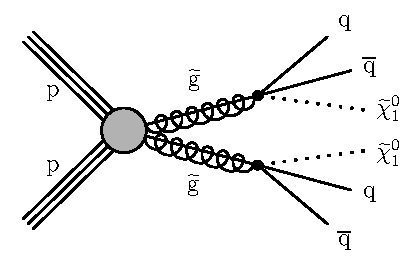
\includegraphics[width=0.3\textwidth]{figures/MT2_2019/Figure_007-a}
    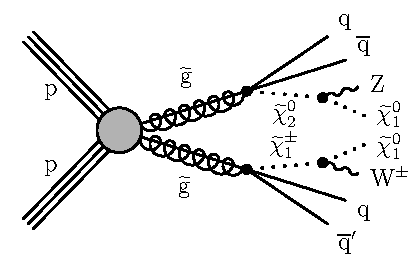
\includegraphics[width=0.3\textwidth]{figures/MT2_2019/Figure_007-b}
    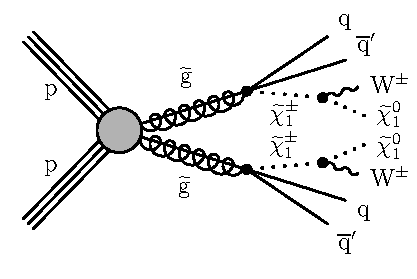
\includegraphics[width=0.3\textwidth]{figures/MT2_2019/Figure_007-c}\\
    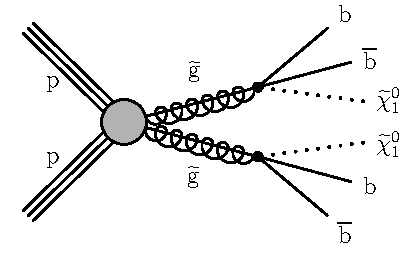
\includegraphics[width=0.3\textwidth]{figures/MT2_2019/Figure_007-d}
    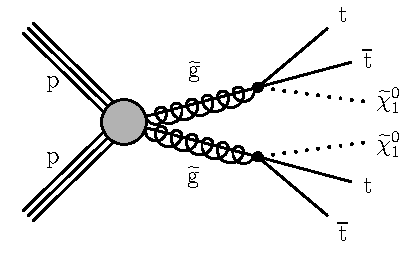
\includegraphics[width=0.3\textwidth]{figures/MT2_2019/Figure_007-e} \\
    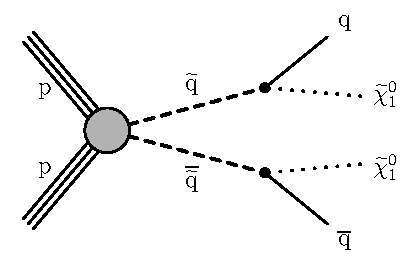
\includegraphics[width=0.3\textwidth]{figures/MT2_2019/Figure_007-f}
    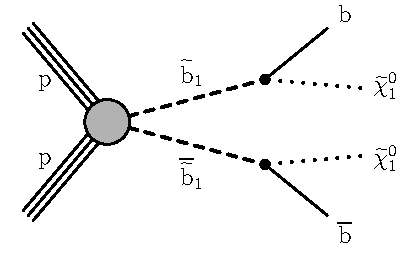
\includegraphics[width=0.3\textwidth]{figures/MT2_2019/Figure_007-g}
    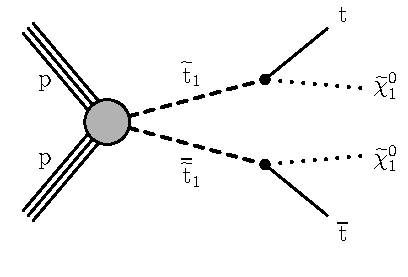
\includegraphics[width=0.3\textwidth]{figures/MT2_2019/Figure_007-h} \\
    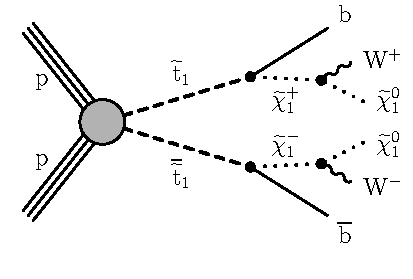
\includegraphics[width=0.3\textwidth]{figures/MT2_2019/Figure_007-i}
    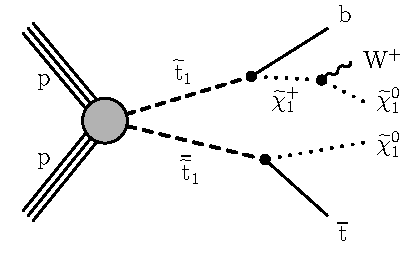
\includegraphics[width=0.3\textwidth]{figures/MT2_2019/Figure_007-j}
    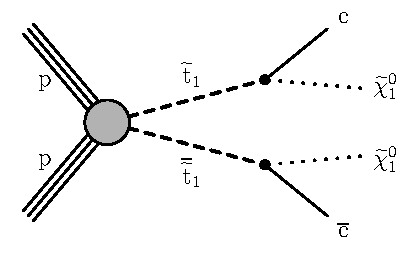
\includegraphics[width=0.3\textwidth]{figures/MT2_2019/Figure_007-k} \\
    \caption[Diagrams for gluino and squark pair production, as predicted by supersymmetric extensions of the Standard Model.]{Diagrams of gluino (upper five) and squark (lower six) pair production, as predicted by supersymmetric extensions of the Standard Model. 
The classic search considers five potential gluino decay chains. 
At upper left, the gluinos decay to light flavor quarks (up, down, strange, or charm), and the lightest neutralino, \lsp.
At upper center, the gluinos decay to light flavor quarks, but rather than decaying directly to \lsp, the gluinos decay either to the second neutralino, \chitwo, which subsequently decays to a Z boson and \lsp, or to the lightest chargino, \chargino, which subsequently decays to the W boson and \lsp, with equal probability.
At upper right, both gluinos undergo the \chargino to W decay chain.
On the left of the second row, both gluinos decay to bottom quark pairs and \lsp.
On the right of the second row, both gluinos decay to top quark pairs and \lsp.
Additionally, the classic search considers six potential modes of squark production and decay.
On the left of the third row, light flavor squarks decay to light flavor quarks and \lsp.
In the center of the third row, bottom squarks decay to bottom quarks and \lsp.
On the right of the third row, top squarks decay to top quarks and \lsp.
At lower left, top quarks decay to bottom squarks and \chargino, which subsequently decay to the W boson and \lsp.
At lower center, top squarks may undergo either the \chargino decay chain, or a direct decay to a bottom squark and \lsp, with equal probability.
At lower right, each top squark decays to a charm squark and \lsp.
Taken from \cite{MT2_2019}.}
    \label{fig:susyproduction}
  \end{figure}  

    The classic search generically targets any new physics that produces high \Ht events with jets and missing energy from undetected particles.
    Diagrams for several candidate models are shown in Figures \ref{fig:susyproduction}, \ref{fig:monophidiag}, and \ref{fig:LQdiags}.
    The diagrams in Figure~\ref{fig:susyproduction} of gluino and squark pair production as predicted by supersymmetric extensions of the Standard Model are of greatest interest, and while the analysis is sensitive to a wide variety of similar hypothetical models, it is optimized for these.
    As discussed in Section \ref{sec:SUSYsms}, these models simplify the enormous parameter space of supersymmetric extensions by assuming that all superpartners except those in the process are so massive that they can be neglected entirely.
    The upper five diagrams all depict pair production of gluinos, the supersymmetric partner of the gluon, the mediating gauge boson of the strong interaction.
    As each gluino decays to two quarks, each of which will typically produce a jet, gluino pair production events tend to have many jets.
    Many different decay chains are possible, and the analysis considers five representative benchmarks.

    In the first benchmark, the gluinos decay to light flavor quarks (up, down, strange, or charm), and the lightest neutralino, \lsp.

    In the second benchmark, the gluinos decay to light flavor quarks, but rather than decaying directly to \lsp, the gluinos can decay either to the second neutralino, \chitwo, which subsequently decays to a Z boson and \lsp, or to the lightest chargino, \chargino, which subsequently decays to the W boson and \lsp.
    Each of these decays can occur with equal probability.
    Both the W and Z will themselves decay, usually to of pair of quarks, which will in turn produce jets. 
    So, relative to the first signal model, the second tends to have greater jet multiplicity.
    The Z can also decay to neutrinos, and the W can decay to a neutrino and a lepton that is not reconstructed.
    In these scenarios, this benchmark trades some jets for an enhanced missing energy signature.
    If  the W or Z decays leptonically and a lepton is successfully reconstructed, events from these signals may fail the lepton veto and instead end up in control regions, biasing the background prediction.
    The procedure used to handle such signal contamination of control regions is described in Section \ref{sec:MT2sigcontam}.

    The third benchmark, in which both gluinos undergo the \chargino to W decay chain, is similar.

    In the fourth benchmark, both gluinos decay to the bottom quark and \lsp.
    As described in Section \ref{sec:btagging}, it is possible to identify jets that originated from a bottom quark; such a jet is said to be ``b-tagged.''
    The classic search bins in the number of b-tagged jets in order to enhance sensitivity to signals of this type.

    In the fifth and final gluino pair-production benchmark, both gluinos decay to top quarks and \lsp.
    The top quark decays with probability near unity to a bottom quark and a W boson.
    The extra W bosons, compared to the direct bottom decay model, can either add jets or leptons and neutrinos, as previously discussed.
    This signal tends to produce the most remarkable events of any signal model considered, with very large \Ht, \njet, and \nb, but also loses many events to the lepton veto as any of the four W bosons is liable to produce a lepton.

    The lower six diagrams of Figure~\ref{fig:susyproduction} all depict pair production of squarks, the supersymmetric partners of quarks.
    Squark decays directly produce only one quark each, compared to two for gluino decays, so squark pair-production events tend to have fewer jets than gluino pair-production events.

    In the first squark benchmark diagram, on the left of the third row, a pair of light flavor squarks (up, down, strange, or charm) is produced and each decays to a light flavor squark and \lsp.
   
    In the second benchmark, bottom squarks are produced and decay to bottom quarks and \lsp.
    These events tend to have b-tagged jets, but fewer than in gluino decays to bottom squarks.

    In the third benchmark, top squarks are pair produced and decay to top quarks and \lsp.
    The relationship between this process and the previous one is similar to the relationship between the fifth and fourth gluino benchmarks, respectively.

    The fourth benchmark is very similar to the third.
    Instead of the top squark decaying directly to a top quark, which then decays to a bottom quark and W boson, the squark decays to a bottom quark directly and \chargino, which subsequently produces the W.
    While the final state particles are identical, their kinematics can be very different depending on the distribution of masses realized in nature.
    For instance, if the top squark and \chargino mass splitting is very small, the bottom quark jet in this benchmark may have such low \pt in a typical event that it is difficult to reconstruct.

    In the fifth benchmark, each top squark may undergo the \chargino decay chain or decay directly to a bottom squark and \lsp, with equal probability, mixing the two previous models.

    In the last benchmark, each top squark decays to a charm quark and \lsp.
    This decay chain could dominate when the top squark and \lsp mass splitting is too small to allow decay to on-shell top quarks, and the mass of \chargino is larger than that of the top squark.

    In each of these models, the mass of the squark or gluino and the mass of \lsp are free parameters.
    Large squark and gluino masses cause low production rates, as the production cross sections drop rapidly with increasing mass, as dicussed in Section \ref{sec:SUSYsms} and shown in Figure~\ref{fig:SUSYxsec}.
    The mass of \lsp does not affect the production rate, except insofar as it must be lower than the masses of all other superpartners, but it does affect the character of the events.
    When the mass splitting between the gluino or squark and \lsp is small, only a small portion of the event's energy ends up in the visible decay products, and most is lost to the rest energy of \lsp.
    These events have low \Ht and \met, low \njet, and when applicable, low \nb, and more closely resemble background.
    As the mass splitting increases, more energy shifts to the visible portion of the event, making events less background-like and increasing sensitivity.
    The analysis considers a grid of potential mass points for each model, and this sensitivity pattern is evident in the curves shown in Section \ref{sec:MT2limits}.
    
    The classic search also considers non-supersymmetric models.

    The first is referred to as the mono-$\phi$ model.
    In this model, a colored scalar boson much like a squark is produced singly, rather than pair-produced as in squark models in order to conserve R-parity, and decays to a quark and invisible fermion, as shown in Figure~\ref{fig:monophidiag}.
    This model has an especially low number of jets and low \mttwo, and so would appear in more background-like bins than most supersymmetric models.
    In fact, it was originally proposed \cite{monophi} to explain a potential excess in bins of this sort in the previous edition of the classic search, published based on 2016 data \cite{MT2_2016}, and so there is some interest in whether such an excess persists in the larger dataset.
    While the analysis is not optimized for models of this sort, indeed \mttwo is designed to target pair-production, it still has some residual sensitivity to any model characterized by jets and missing energy in the final state, including mono-$\phi$.

    The second non-supersymmetric model, and final model considered explicitly by the classic search, is leptoquark extensions of the Standard Model.
    As discussed in Section \ref{sec:othermodels}, while squarks can decay to a quark and \lsp, leptoquarks decay to a quark and a neutrino, which is experimentally effectively indistinguishable from a low mass \lsp.
    This last fact was first established in a reinterpretation of the 2016 edition of the classic search \cite{LQ2016}.
    Thus, it is a relatively simple exercise to reinterpret squark squark results in the low mass \lsp limit to leptoquark results.
    A few leptoquark production diagrams are shown in Figure~\ref{fig:LQdiags}.

  \begin{figure}[h!]
    \centering
    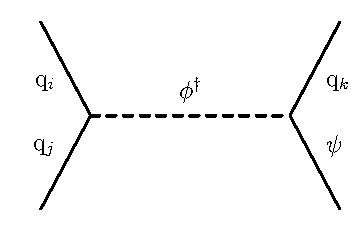
\includegraphics[width=0.85\textwidth]{figures/MT2_2019/Figure_008.pdf}
    \caption[Diagram for the mono-$\phi$ model.]{Diagram for the mono-$\phi$ model, in which a colored scalar $\phi$ is resonantly produced, and decays to an invisible massive Dirac fermion $\psi$ and an SM quark. Note that $\phi$ is not pair-produced, in contrast to otherwise-similar squarks. Taken from \cite{MT2_2019}.}
    \label{fig:monophidiag}
  \end{figure}  

  \begin{figure}[h!]
    \centering
    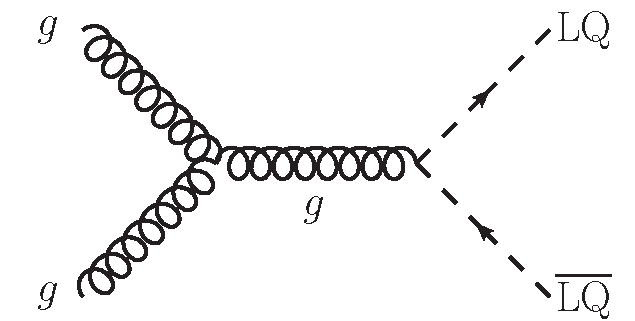
\includegraphics[width=0.3\textwidth]{figures/MT2_2019/Figure_009-a}
    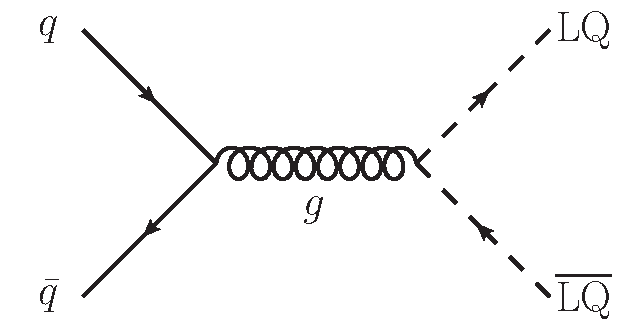
\includegraphics[width=0.3\textwidth]{figures/MT2_2019/Figure_009-b}\\
    \vspace{3mm}
    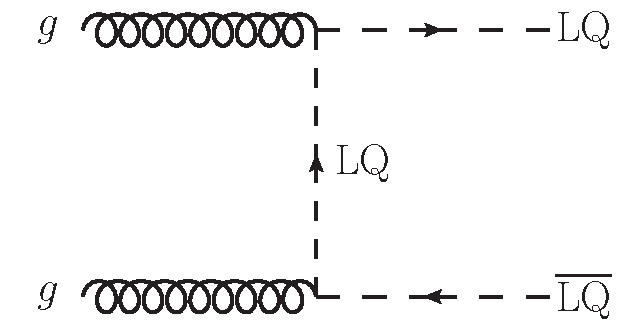
\includegraphics[width=0.3\textwidth]{figures/MT2_2019/Figure_009-c}
    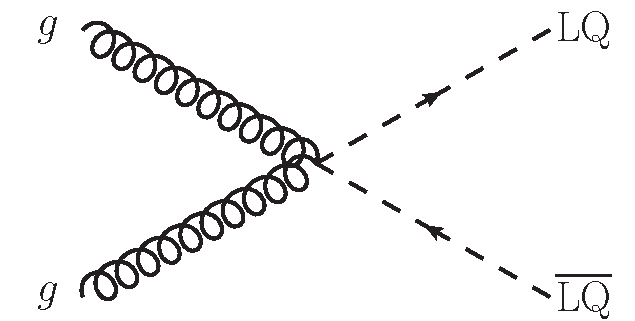
\includegraphics[width=0.3\textwidth]{figures/MT2_2019/Figure_009-d}
    \vspace{3mm}
    \caption[Leptoquark pair production diagrams.]{Diagrams of leptoquark pair production. Each lepqtoquark decays to a neutrino and a quark. Taken from \cite{MT2_2019}.}
    \label{fig:LQdiags}
  \end{figure}  

  \subsection{Backgrounds} \label{sec:MT2bg}

  All of the targeted signals are characterized by all-hadronic events with large missing energy, but observing such an event does not constitute discovery due to the existence of backgrounds that can produce the same basic signature.
  These backgrounds can be broadly divided into the detector mismeasurement background, in which apparent missing energy is generated not by genuine undetected particles but by an error in reconstruction, and the neutrino background, in which the missing energy is produced by genuine neutrinos as predicted in the Standard Model.
  The neutrino background can be subdivided into neutrinos originating from $W^{\pm}\rightarrow \ell^{\pm}\nu$, in which the presence of a charged lepton allows the neutrino to be rejected with good efficiency, and those originating from $Z\rightarrow \nu\nu$, in which the final state is entirely invisible and cannot be efficiently vetoed.

  
    \subsubsection{Mismeasurement} \label{sec:MT2QCD}
  
    The most problematic background is that caused by detector mismeasurement.
    Nearly every mismeasured event is a QCD multijet event, because nearly every event at a proton-proton collider is a QCD multijet event and the probability of mismeasurement is roughly flat across events. 
    Accordingly, the mismeasurement background is also referred to as the QCD multijet background.
    While the detector makes mistakes only very rarely, QCD events are so relatively common that this background is still dominant in the raw dataset, before any cleaning selections.

    Estimating the QCD background is challenging because it requires highly detailed knowledge of the detector's idiosyncracies.
    Rather than risk falsely discovering a signal or failing to identify one that is present due to misprediction of this background, the analysis adopts selections designed to suppress it, until the background is sufficiently minor that large relative error in its prediction is acceptable.
    
    The first and most powerful of these selections uses the \mttwo variable described in Section \ref{sec:MT2}, namely $\mttwo > 200$~GeV, where the value is chosen to achieve the desired suppression of the mismeasurement background.
    Although the \mttwo selection is somewhat expensive in the sense that it eliminates a significant fraction of signal, especially for signals with a small mass splitting and signals like mono-$\phi$ that are not pair-produced, it is crucial for suppressing the mismeasurement background.
    At $\Ht > 1500$~GeV, the mismeasurement background extends unacceptably beyond $\mttwo \sim 200$~GeV, and the \mttwo selection is tightened to $\mttwo > 400$~GeV.

    The second selection uses the observable 
    $$\dphimin = \textrm{Min}\left(\left|\phi_{\met}-\phi_i\right|\right)$$
    where $\phi_i$ indicates the $\phi$ coordinate of the $i$th \pt jet and $\phi_{\met}$ is the $\phi$ coordinate of the missing energy vector.
    Stated simply, \dphimin is the smallest angular separation in the transverse plane of the missing energy vector and any of the four highest \pt jets.
    Close overlap between a jet and the missing energy vector indicates a high probability that the jet was badly mismeasured, and is itself the source of the \met in the event.
    The selection applied is $\dphimin > 0.3$, where the value is chosen to achieve strong background rejection without too great a loss of signal efficiency.
    Only the four highest energy jets are used because the probability of {\it some} jet overlapping the missing energy vector approaches unity as the number of jets increases, so the selection would nearly always veto high \njet\xspace events, and the high \njet\xspace bins are sufficiently signal-rich that aggressive background rejection is not as necessary.
    The effect of this selection is depicted in Figure~\ref{fig:dphimin}, after an \mttwo selection of only 100 GeV.

    The last selection rejects events in which a suspiciously large fraction of the missing energy comes from very soft objects.
    The minimum \pt for selected jets is 30~GeV.
    The missing energy vector from only jets is denoted $\vec{\HTm}$.
    The missing energy vector used in the analysis, $\vec{\met}$, uses all PF candidates, including those outside jets or in jets with $\pt < 30$~GeV.
    If these two quantities are very different, it means that a large portion of the \met in the event was generated by these low \pt objects, a sign that something may have gone wrong in reconstruction.
    Specifically, the selection is $\left|\vec{\HTm}-\vec{\met}\right|/\met < 0.5$.

    \begin{figure}[h!]
      \centering
      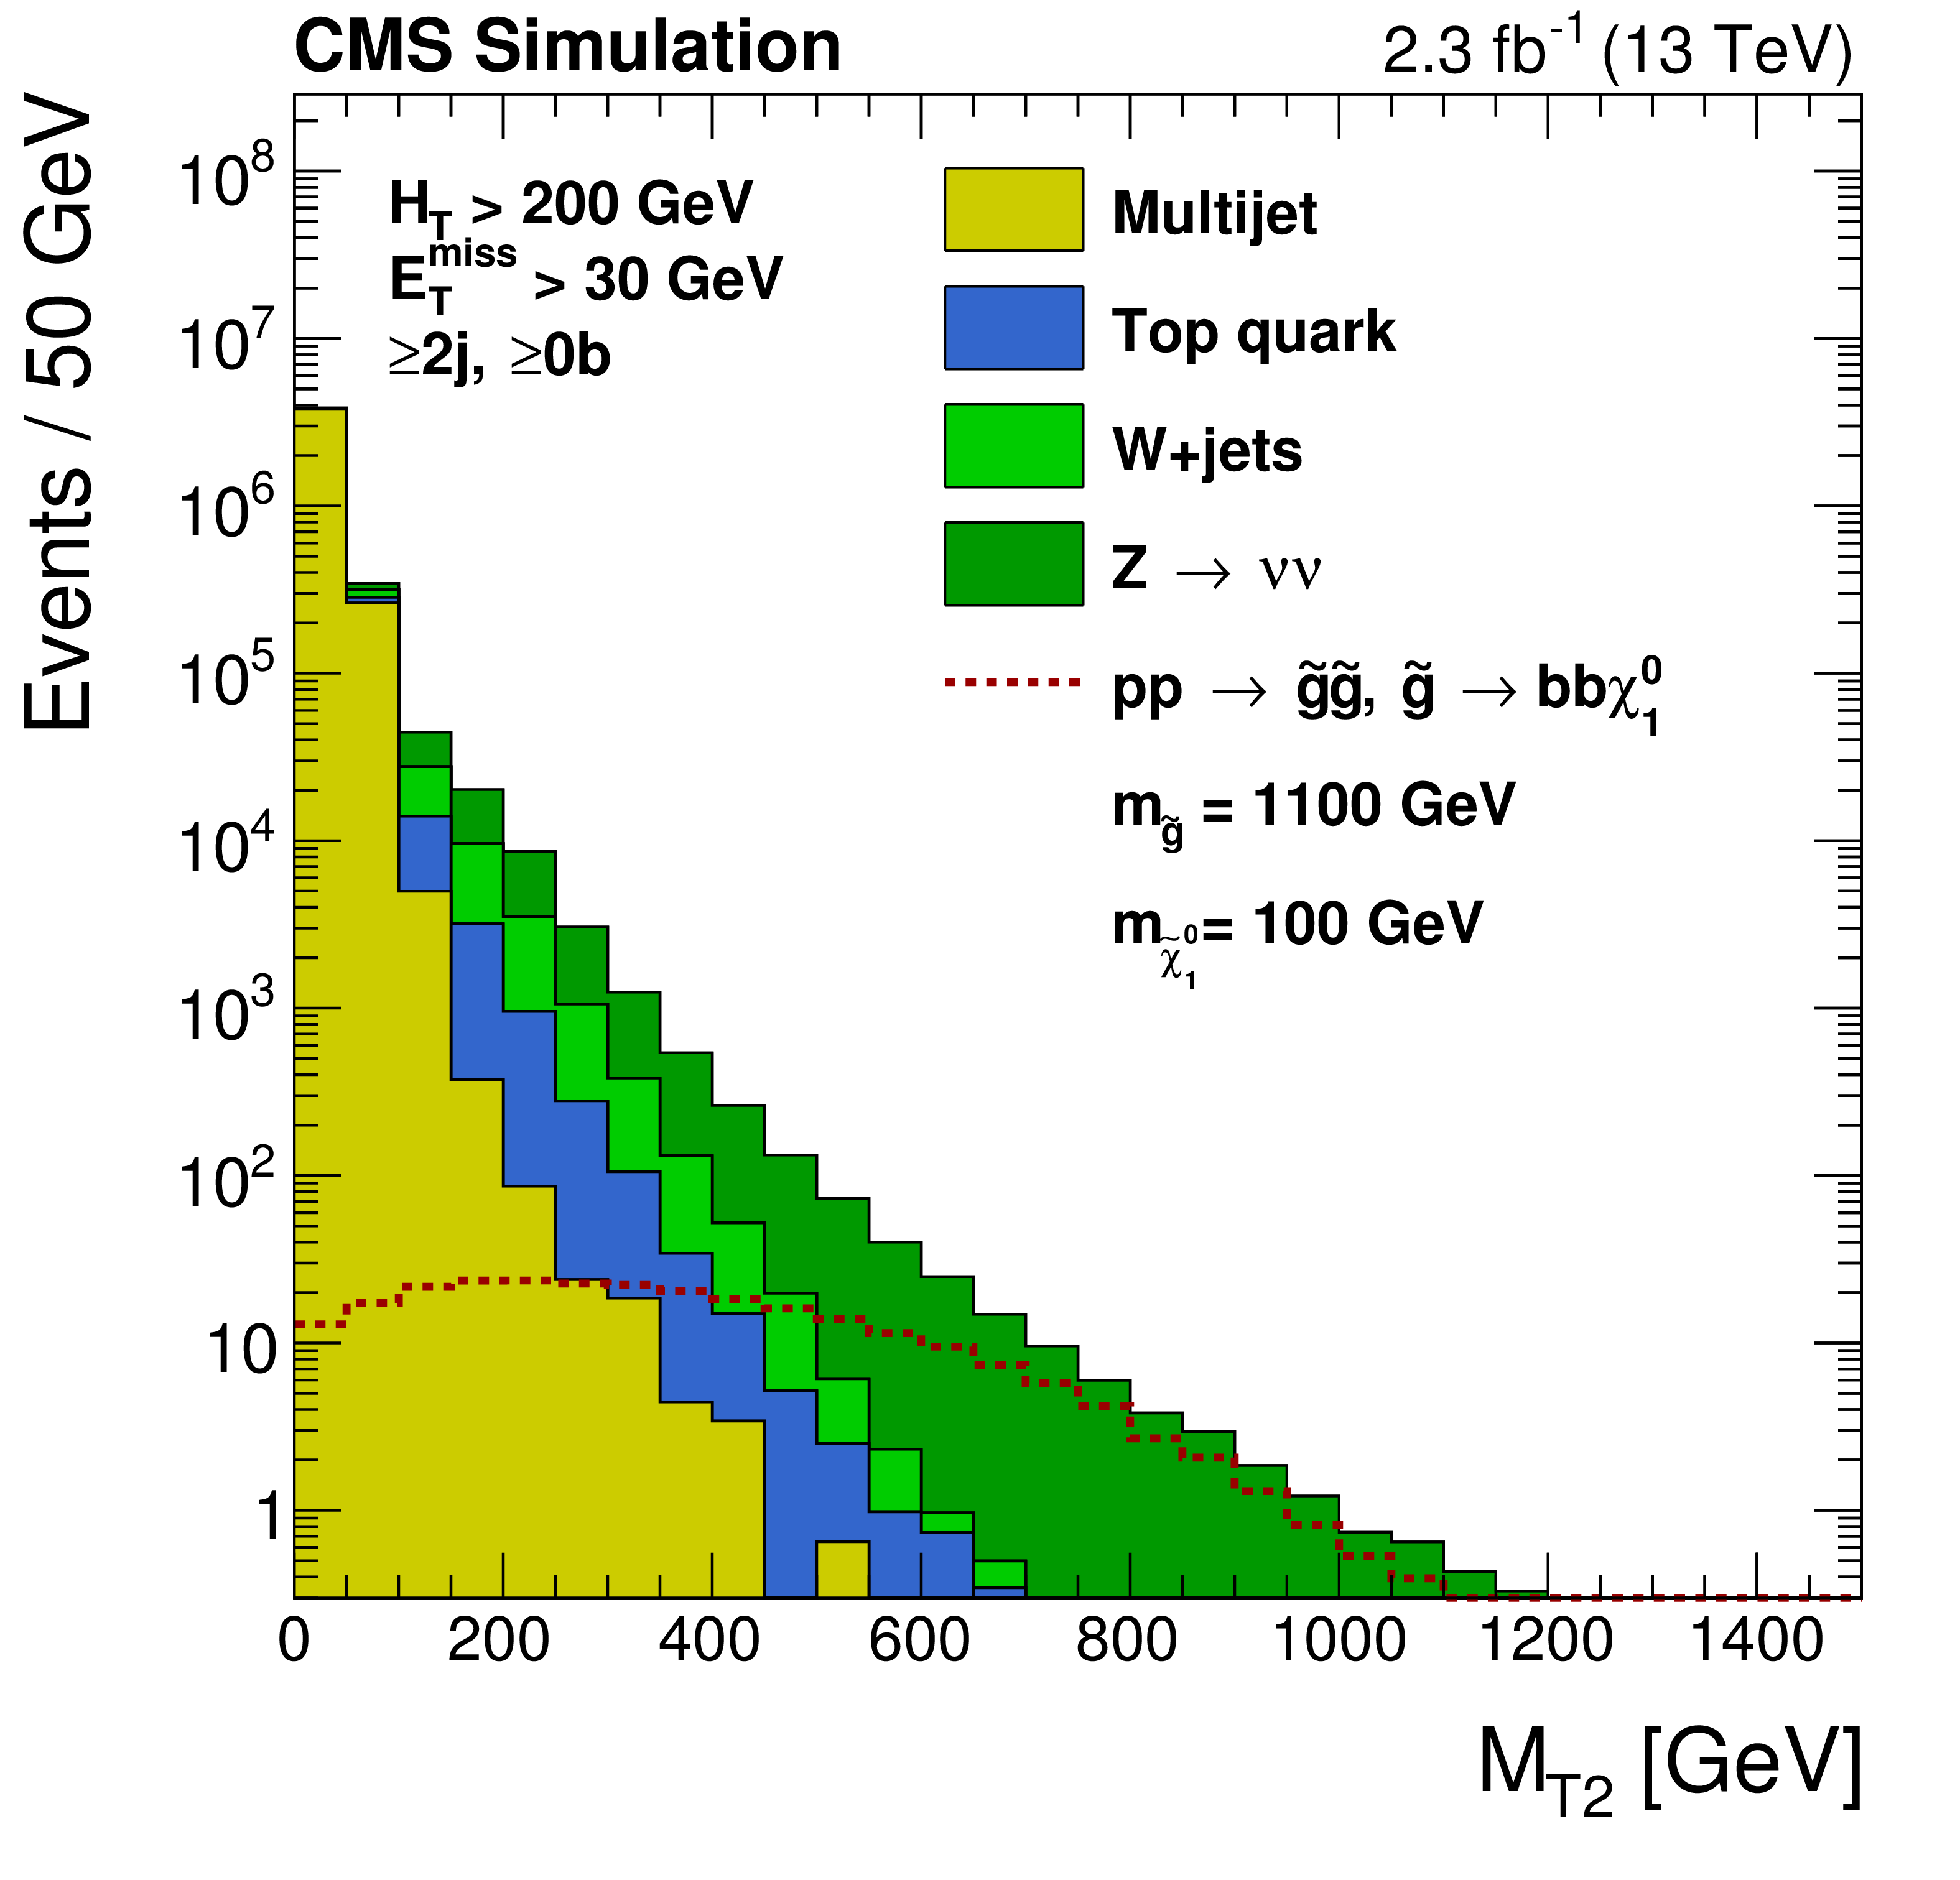
\includegraphics[width=0.48\textwidth]{figures/mt2_mt2_2015.png}
      \caption[\mttwo distributions of backgrounds and an example signal point.]{The distributions in \mttwo of the QCD background (filled yellow) and the neutrino backgrounds (filled blue and green) are stacked and overlaid with an example signal point (gluino pair production and decay to bottom quarks, in red). Even with other mismeasurement-suppression selections applied, the mismeasurement background still dominates without $\mttwo > 200$~GeV. Taken from \cite{MT2_2015}.}
      \label{fig:mt2dist}
    \end{figure}  
    
    \begin{figure}[h!]
      \centering
      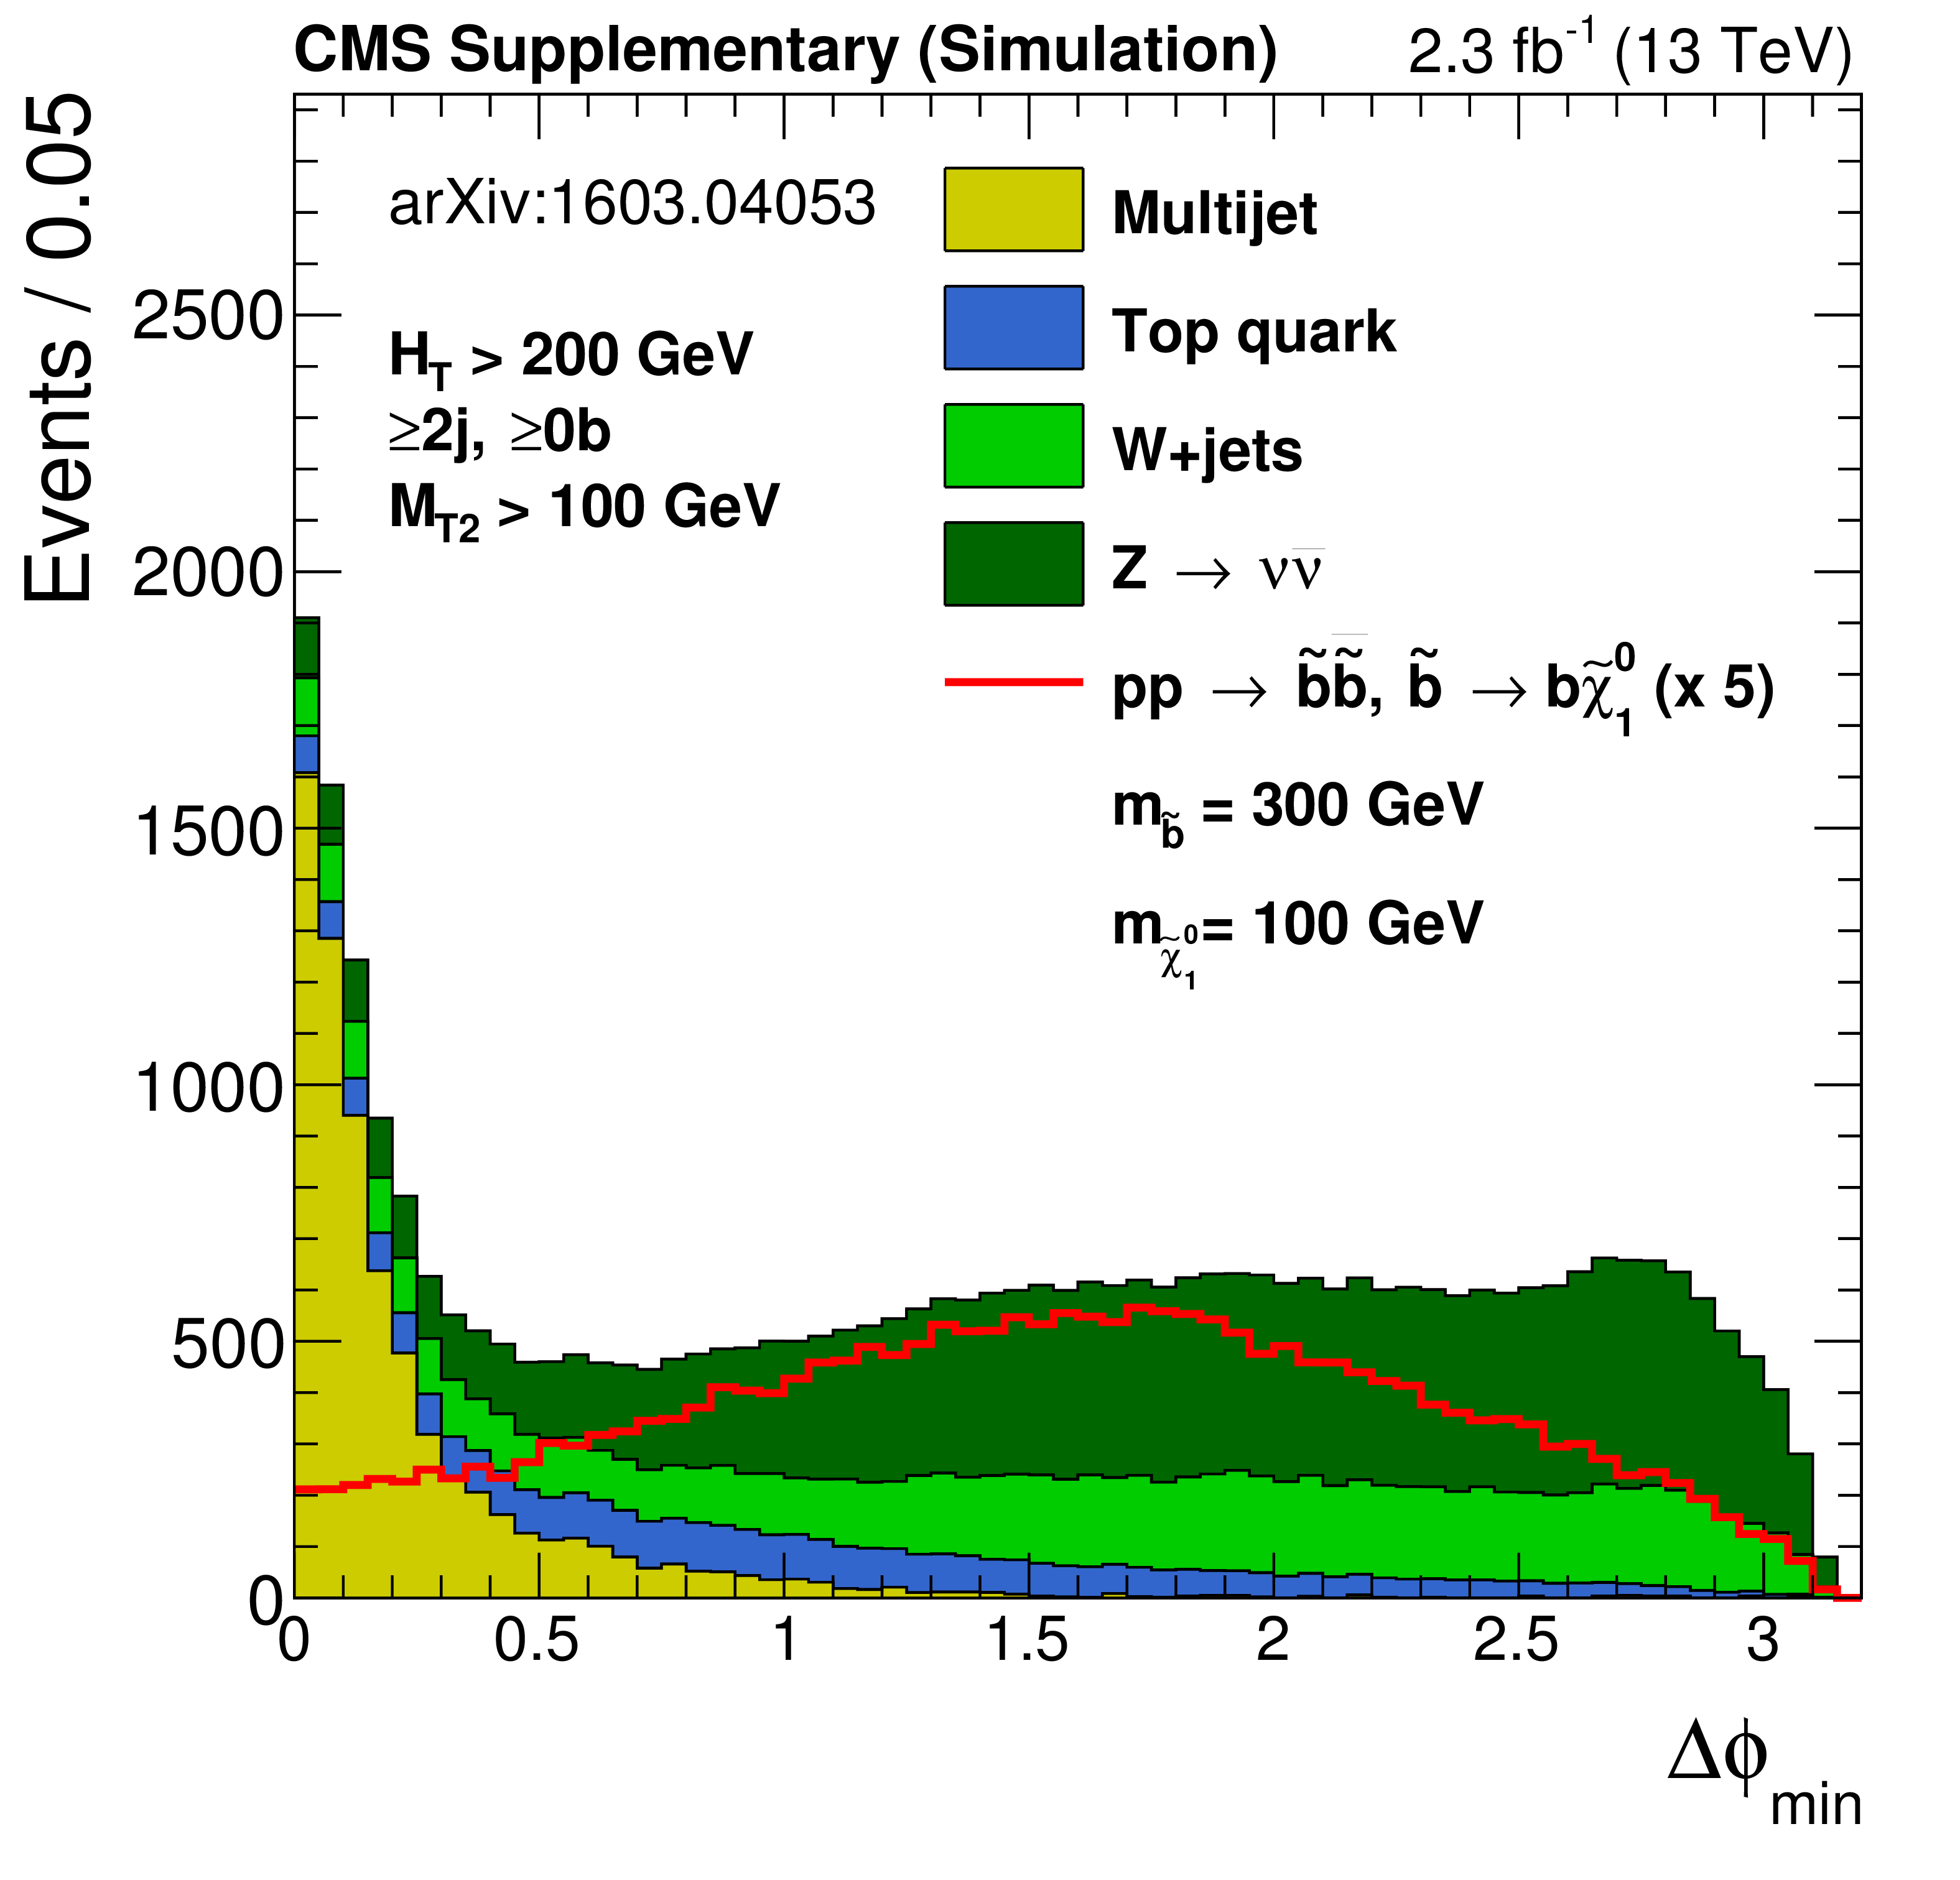
\includegraphics[width=0.48\textwidth]{figures/mt2_dphi_2015.png}
      \caption[\dphimin distributions of backgrounds and an example signal point.]{The distributions in \dphimin of the QCD background (filled yellow) and the neutrino backgrounds (filled blue and green) are stacked and overlaid with an example signal point scaled up by a factor of 5 (bottom squark pair production, in red), with the \mttwo selection relaxed to 100 GeV. Note that most QCD lies below the cut value of 0.3. Taken from \cite{MT2_2015} supplementary materials.}
      \label{fig:dphimin}
    \end{figure}  
    
    The residual mismeasurement background is estimated using a procedure called Rebalance and Smear that was newly implemented for this edition of the classic analysis, and described in Section \ref{sec:RandS}.
    
    \subsubsection{Lost Lepton} \label{sec:MT2lostlep}

    The lepton veto rejects most events containing neutrinos originating from the decay of a W boson, $W^{\pm}\rightarrow \ell^{\pm}\nu$.
    However, the lepton is not always successfully reconstructed, usually because the lepton is a $\tau$ that decays hadronically and is mistaken for a meson, and this residual so-called lost lepton background must be estimated. 

    A first attempt might be to simulate events containing W bosons, scale the simulation to the desired luminosity, and count the events in which the lepton is not reconstructed.
    This procedure would have reasonable accuracy, but producing accurate simulations is not trival, and the result would be subject to an array of systematic errors.
    Schematically, if $N_{LL}^{Data}$ is the actual number of lost lepton events in data and $N_{LL}^{MC}$ is the number predicted by Monte Carlo simulation, the simulation will mispredict by some factor $\epsilon$ such that $N_{LL}^{Data} = \epsilon N_{LL}^{MC}$.

    It is possible to do better than $\epsilon$ with data driven techniques.
    In addition to the lost lepton events, one can also ask the simulation for its prediction of the number of W events in which the lepton is not lost, single lepton events, $N_{SL}^{MC}$, where we restrict the lepton to electrons and muons since $\tau$ reconstruction is much more difficult.
    Every part of this simulation is exactly identical to the lost lepton simulation, subject to almost the same errors, with the major exception being the predicted lepton reconstruction efficiency.
    Call this new error factor $\delta$ so that $N_{SL}^{Data}=\delta N_{SL}^{MC}$.
    Then $\epsilon/\delta = \gamma$ is the portion of the misprediction due to the simulation's imperfect knowledge of the lepton reconstruction efficiency and a few other more minor uncorrelated effects, a small portion of the total.
    The ratio $R_{MC}^{0\ell/1\ell} = N_{LL}^{MC} / N_{SL}^{MC}$ is subject only to this relatively small error $\gamma$, since the fully correlated errors cancel.
    The prediction of $N_{LL}^{Data}$ follows directly,
    \begin{equation}
      N_{LL}^{Data;Est} = R_{MC}^{0\ell/1\ell} N_{SL}^{Data}.
    \end{equation}
    The input $N_{SL}^{Data}$ is measured in a control region populated by single lepton events observed in data, in a kinematic region identical to the corresponding lost lepton signal region.
    The remaining systematic uncertainty is only about 15\% in most signal regions.

    While the lost lepton background tends to be subdominant relative to the Invisible Z background discussed in the next section, it is the largest background in certain high \njet, high \nb, high \Ht bins as Z events do not populate these bins efficiently, while $t\bar{t}$ pair-production events do, and all $t\bar{t}$ events contain two W bosons that may decay leptonically.

    \subsubsection{Invisible Z} \label{sec:MT2zinv}

    The $Z\rightarrow \nu\nu$ background is predicted in a similar fashion to the lost lepton background, using a control region populated with $Z\rightarrow \ell^+\ell^-$ events.
    Again, the leptons are restricted to pairs of electrons and pairs of muons, since $\tau$ reconstruction is much more difficult.    
    Figure~\ref{fig:Zestimate} (right) shows the similarity in the \mttwo distributions of simulated \znunu events and observed \zll events in which one pretends that the leptons are invisible, demonstrating both that these events are kinematically very similar as expected, and that the simulation is accurate.
    The ratio $R_{MC}^{\nu\nu/\ell^+\ell^-}$ can be extracted from Monte Carlo simulation, and is dominated by only the lepton reconstruction efficiency uncertainty.
    In the Standard Model, this ratio is almost exactly 3, but it is significantly larger experimentally because it is possible for one of the leptons in $Z\rightarrow\ell^+\ell^-$ not to be well-reconstructed, causing the affected event not to be counted.
    The value $N_{\ell^+\ell^-}^{Data}$, unlike $N_{SL}^{Data}$, is not trivial to extract, since a non-negligible fraction of double lepton events come from sources other than a single Z boson, 
    almost always one each from a pair of W bosons.
    $N_{\ell^+\ell^-}^{MC}$ and $N_{\nu\nu}^{Data}$ are exclusively $Z\rightarrow \ell^+\ell^-$ and $Z\rightarrow\nu\nu$ events, respectively, and for maximal cancellation of systematic uncertainties, it is desirable that $N_{\ell^+\ell^-}^{Data}$ be purified to the greatest extent possible.

  \begin{figure}[h!]
    \centering
    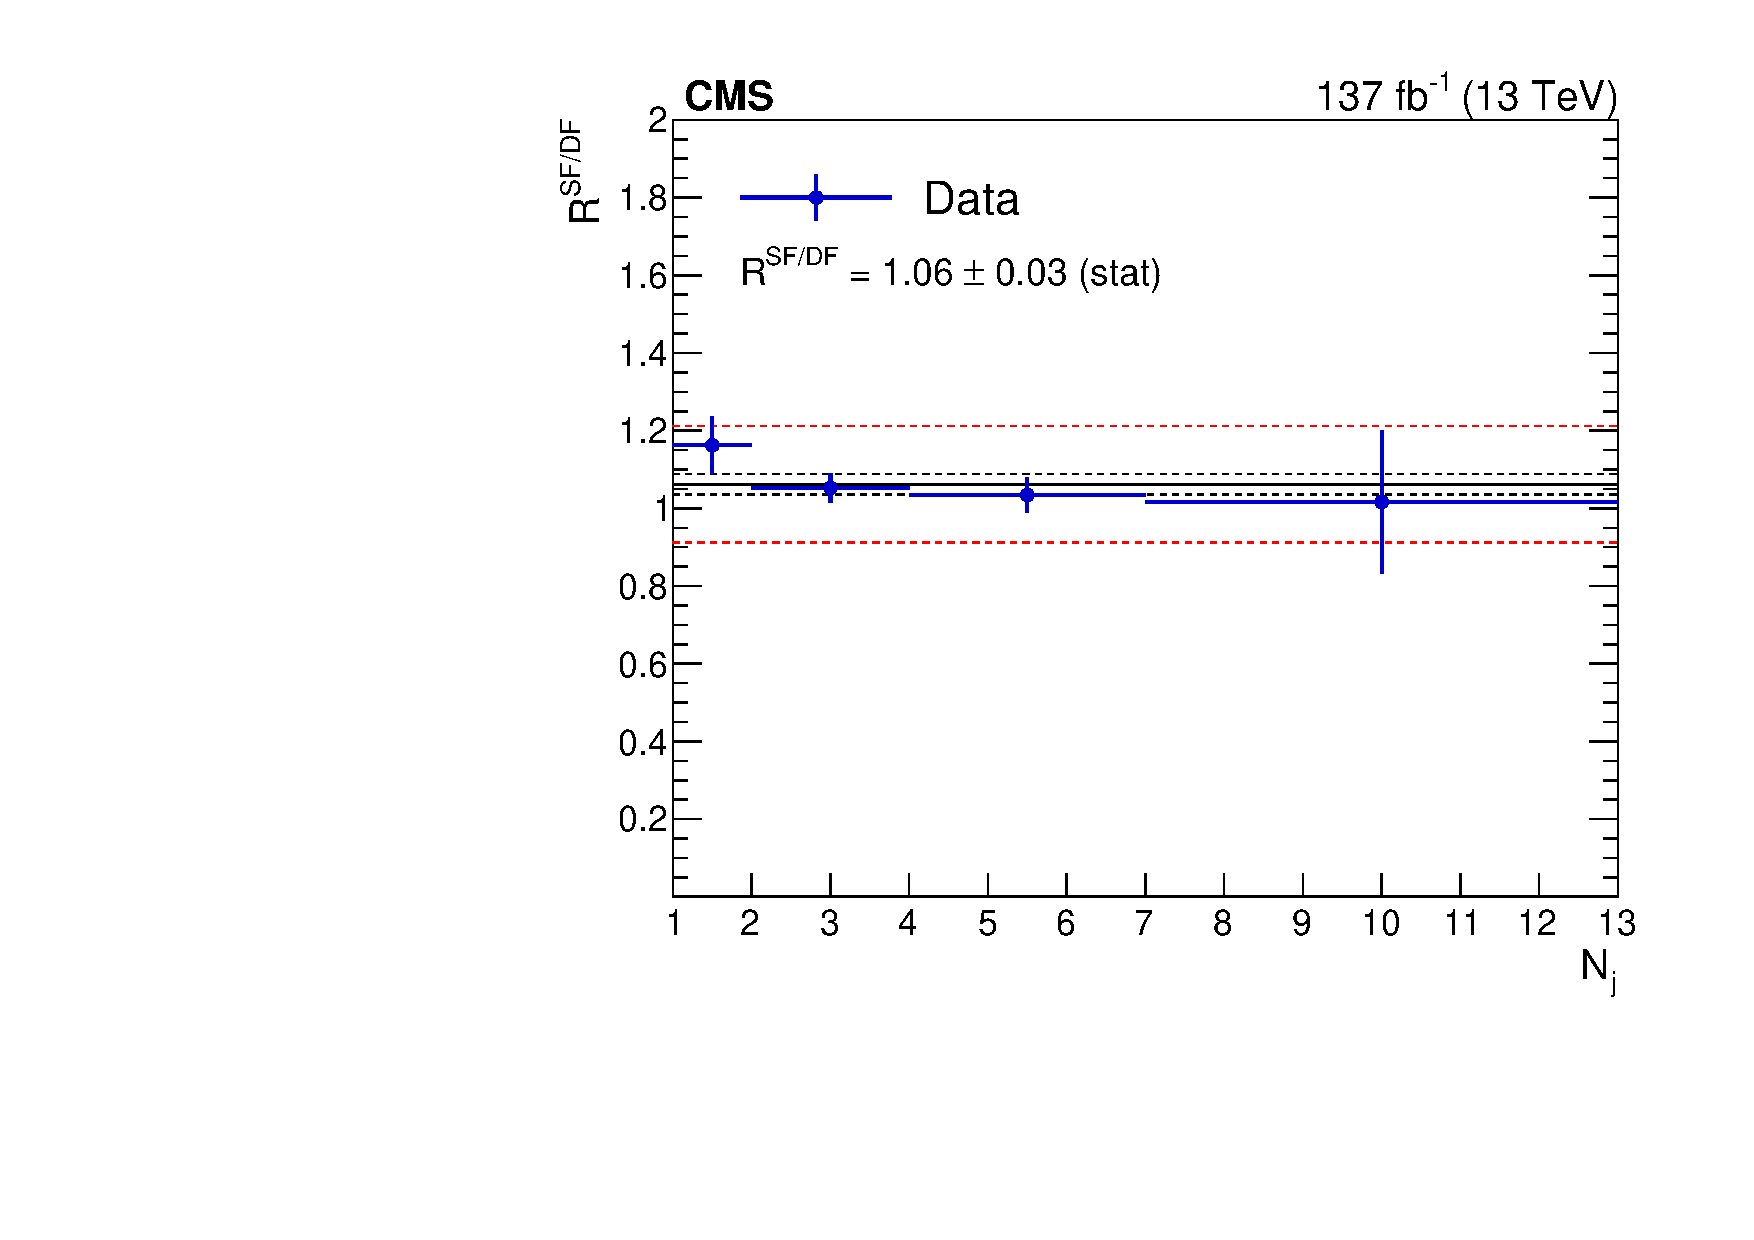
\includegraphics[width=0.53\textwidth]{figures/MT2_2019/Figure_002-a.pdf}
    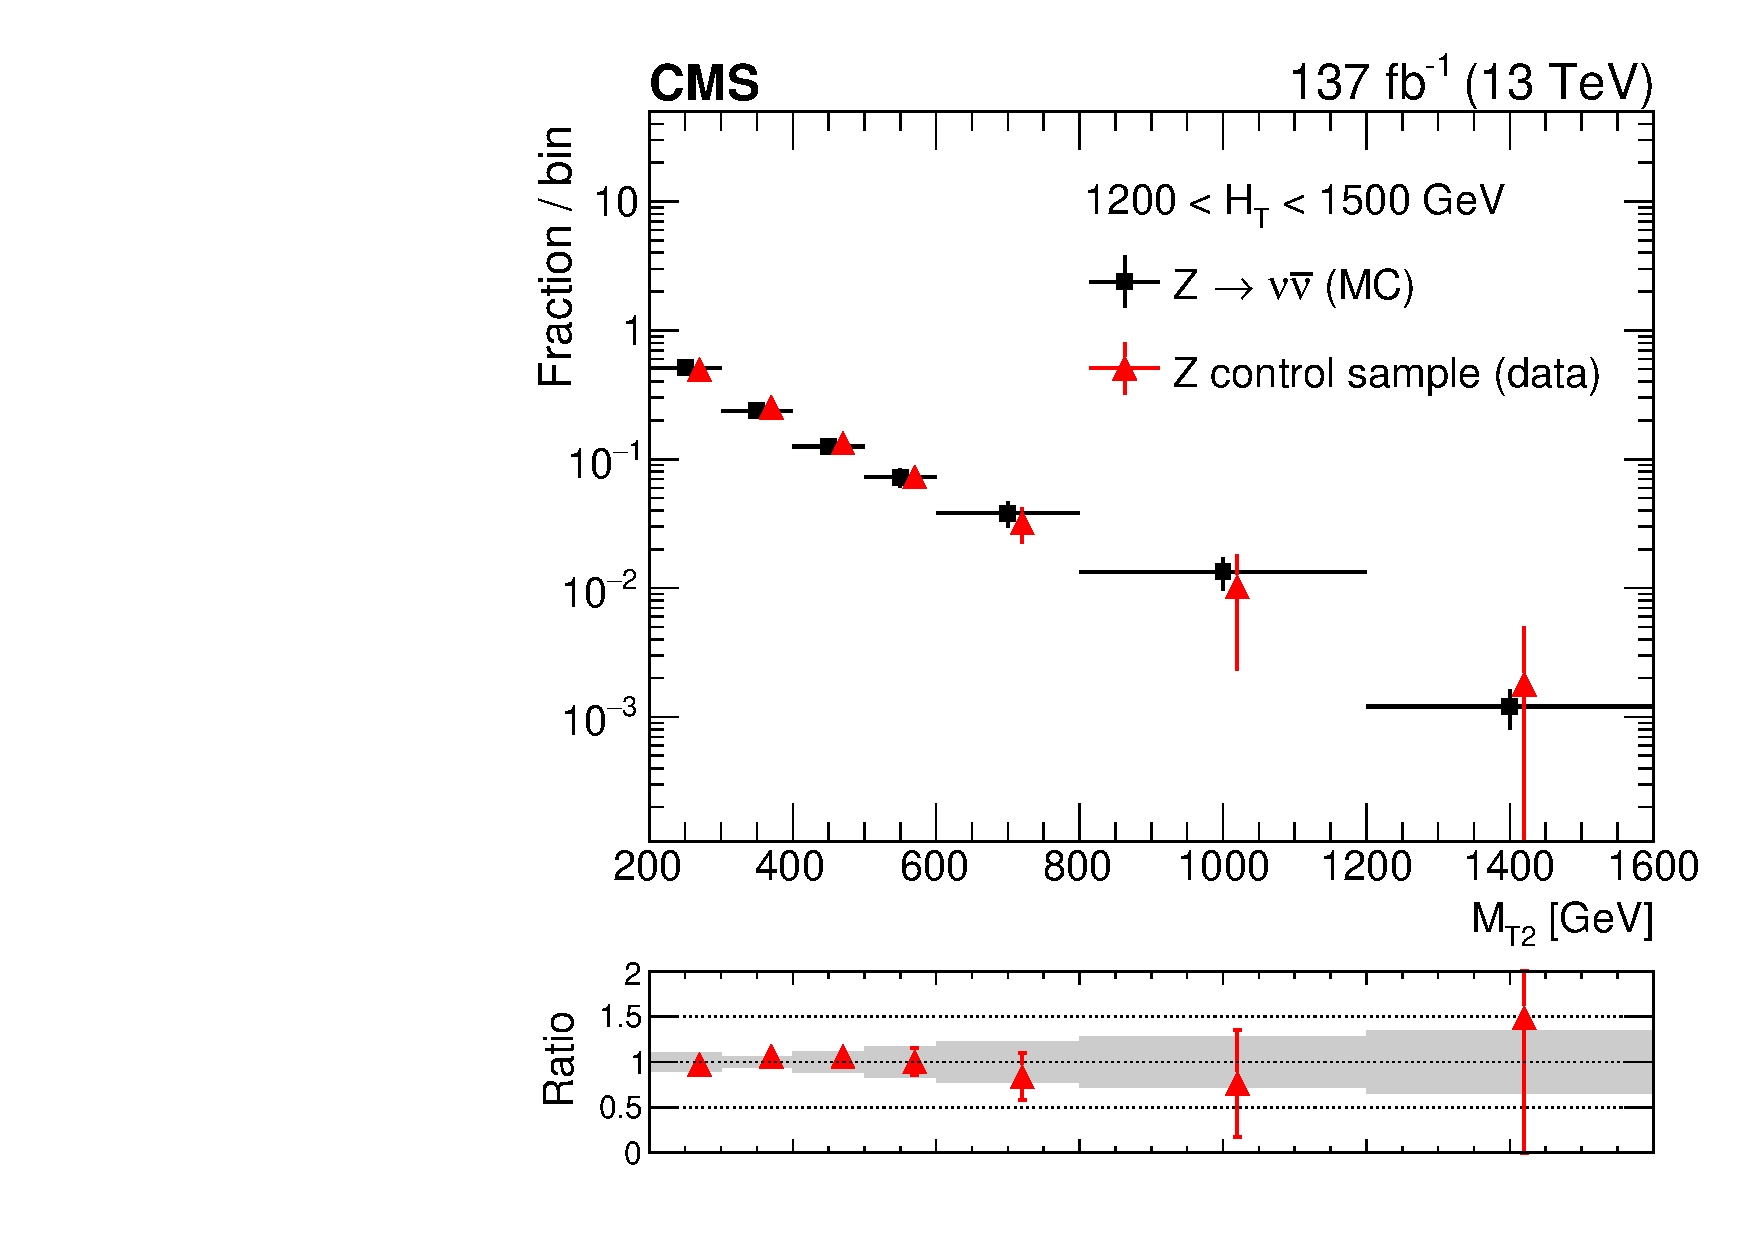
\includegraphics[width=0.44\textwidth]{figures/MT2_2019/Figure_002-b.pdf}
    \caption[(Left) The ratio of the number of same flavor to different flavor lepton pairs in data. (Right) A comparison of the \Mttwo shape between data Z to lepton events and simulated Z to neutrino events.]{
      (Left) The ratio of the number of same flavor to different flavor lepton pairs in data, $R^{SF/DF}$, which is a component of the $Z\rightarrow\nu\nu$ background estimate from $Z\rightarrow\ell^+\ell^-$ events. (Right) A comparison of the \Mttwo shape between data $Z\rightarrow\ell^+\ell^-$ events and simulated $Z\rightarrow\nu\nu$ events. The two processes should be kinematically identical, and the similarity of the distributions indicates that the Monte Carlo simulation models the processes well. Taken from \cite{MT2_2019}.}
    \label{fig:Zestimate}
  \end{figure}  

    Fortunately, there is an experimental handle on the contamination.
    When a Z boson decays to a lepton pair, the flavor is always identical, either two electrons or two muons.
    When a pair of W bosons each decay to a lepton pair, their choices are uncorrelated.
    Half the time, the flavors will be identical as for a Z event, and half the time, one W will decay to a muon and the other to an electron.
    The first case is the undesired impurity in $N_{\ell^+\ell^-}^{Data}$, and events of the second type are used to populated a different-flavor control region used to predict the impurity, $N_{DF}^{Data}$.
    It is nearly sufficent simply to subtract $N_{DF}^{Data}$ from $N_{\ell^+\ell^-}^{Data}$ since the different flavor and same flavor W events occur at the same rate.
    However, it is possible that the detector is slightly more or less efficient at reconstructing events where both leptons are the same flavor than events in which they are different flavors, so the different flavor count must be scaled slightly to compensate, by a factor $R^{SF/DF}$.
    $R^{SF/DF}$ is measured in data in $\ell^+\ell^-$ events that are kinematically inconsistent with originating from a Z decay, chiefly due to a requirement that the invariant mass of the lepton pair be at least 20~GeV away from the Z mass.
    One finds that $R^{SF/OF} \approx 1.06 \pm 0.15$, as shown in Figure~\ref{fig:Zestimate} (left).
    The final prediction is
    \begin{equation}
      N_{\nu\nu}^{Data;Est} = R_{MC}^{\nu\nu/\ell^+\ell^-}(N_{Data}^{\ell^+\ell^-}-R^{SF/OF}N_{DF}^{Data})
    \end{equation}
    Being irreducible, the \znunu plus jets background is dominant in the vast majority of bins.

  \subsection{Baseline Selection} \label{sec:MT2baseline}

  \begin{table}[htbp]
    \scriptsize
    \centering
    \renewcommand{\arraystretch}{1.3}
    \begin{tabular}{c c l}
      Observable               & Selection   & Notes \\
      \hline
      \mttwo                   & $> 200$~GeV & Only for multijet events. Increased to $\mttwo > 400$~GeV for $\Ht > 1500$~GeV to maintain QCD suppression. \\
      $\pt^{\mathrm{Jet 1}}$   & $> 250$~GeV & Only for monojet events. \\
      \Ht                      & $> 250$~GeV & Motivated by available triggers. Background events at lower \Ht are too common for these events to be always recorded. \\
      \met                     & $> 250$~GeV & Relaxed to $\met > 30$~GeV for $\Ht > 1200$~GeV. Motivated by available triggers. \\
      \dphimin                 & $> 0.3$     & Auxiliary mismeasurement suppression. \\
      $\left|\vec{\HTm} - \vec{\met}\right|/\met$ & $< 0.5$ & Auxiliary mismeasurement suppression. \\
      \nlep                    & $= 0$       & The lepton veto; rejects the majority of $W^{\pm}\rightarrow\ell^{\pm}\nu$ background. \\
    \end{tabular}
    \caption[Summary table of baseline event selection.]{A summary of the baseline event selection for the classic \mttwo search.
      Events are required to have large \Ht, no leptons, and significant missing energy unlikely to be the product of detector mismeasurement or a single undetected particle.}
    \label{tab:baseline}
  \end{table}

  The properties of these signals and backgrounds motivate the baseline event selection summarized in Table \ref{tab:baseline}.
  The \mttwo selection primarily suppresses the mismeasurement background, by many orders of magnitude.
  The \dphimin and \HTm selections also help to suppress this background further, until it is smaller than the genuine \met backgrounds.
  The \Ht and \met selections are chosen primarily so that all of the selected events pass the online trigger.
  Backgrounds are so common at $\Ht < 250$~GeV, and $\met < 250$~GeV for $\Ht < 1200$~GeV, that the experiment is unable to record all of the events observed, making this part of the parameter space a poor region to search for a rare signal in any case.
  The lepton veto rejects most $W^{\pm}\rightarrow\ell^{\pm}\nu$ events, so that only events in which the lepton is not reconstructed remain in the signal region, as described in Section \ref{sec:MT2lostlep}, and serves to narrow the analysis' focus to the all-hadronic final state as part of CMS's larger research program.

  In addition to this baseline selection, the analysis bins in \mttwo, \Ht, \njet, and \nb to enhance signal sensitivity as described in Section \ref{sec:newbinning}.

  \subsection{Upgrades in 2019} \label{sec:MT2upgrades}

  The classic search has been performed before at 13 TeV, once in 2015 \cite{MT2_2015} using a 2.3~\fbinv dataset, and again in 2016 \cite{MT2_2016} using 35.9~\fbinv.
  The update in 2019 uses the full dataset from 2016, 2017, and 2018, totaling 137~\fbinv.
  As the analysis is dominated by statistical uncertainties in its most sensitive bins, the increased statistical power is the primary improvement in the update.
  
  The update includes two other major upgrades.

  The first improves the estimate of the mismeasurement background using a technique called Rebalance and Smear.

  The second leverages the increased statistics to expand the signal region binning, better targeting signal models with more extreme jet and b-tagged jet multiplicities, and \mttwo.
  

    \subsubsection{Rebalance and Smear} \label{sec:RandS}

    \begin{figure}[h!]
      \centering
      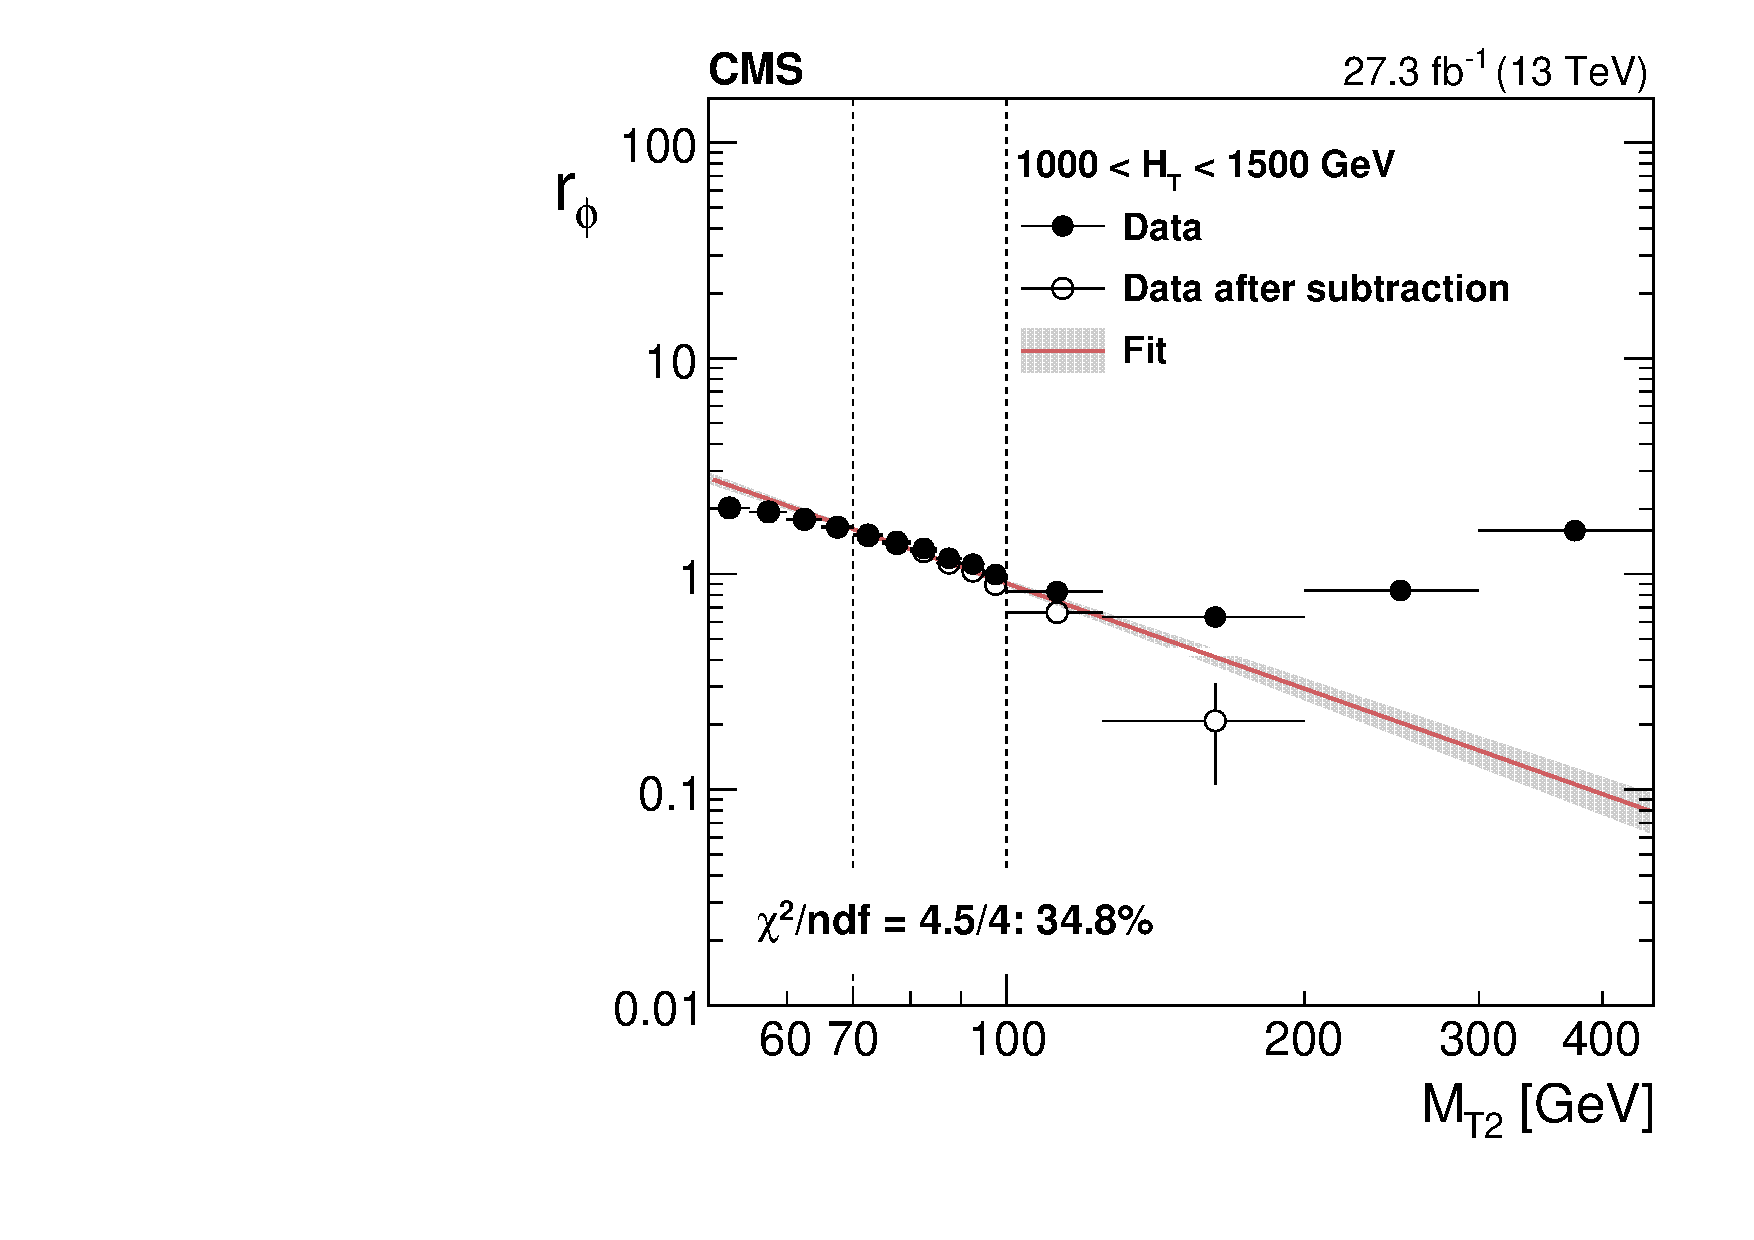
\includegraphics[width=0.85\textwidth]{figures/mt2_rphi_2016.pdf}
      \caption[Fit of $r_{\phi}$ as a function of \mttwo.]{
        The fit of $r_{\phi} = N_{\dphimin > 0.3}/N_{\dphimin < 0.3}$ as a function of \mttwo obtained in the 2016 classic search, for the $1000 < \Ht < 1500$~GeV \Ht band. 
        The fit is performed in events in the \mttwo band $70 < \mttwo < 100$~GeV and extrapolated to the $\mttwo > 200$~GeV signal region.
        Black points represent raw data, while white points represent data after the non-multijet contribution is subtracted.
        Taken from \cite{MT2_2016}.}
      \label{fig:rphi}
    \end{figure}  

    In older versions of the classic search \cite{MT2_2015, MT2_2016}, the mismeasurement background estimate used the \dphimin observable and extrapolated across \mttwo.
    Events at low \mttwo and at low \dphimin are both dominated by QCD mismeasurement.
    The suppression effect of \mttwo is so strong that even events at low \mttwo and {\it high} \dphimin are QCD dominated.
    As essentially every low \mttwo event is a QCD event, low \mttwo events can be used to measure the ratio $r_{\phi}$ of QCD mismeasurement events at high and low \dphimin.
    High \mttwo events with low \dphimin can then serve as a control region for estimating the QCD mismeasurement background, $N_{\dphimin > 0.3} = r_{\phi} N_{\dphimin < 0.3}$.
    Unfortunately, $r_{\phi}$ decreases with increasing \mttwo, so that instead the dependence must be fit to a power law at low \mttwo and extrapolated to high \mttwo, as shown in Figure~\ref{fig:rphi}.
    This procedure has obvious potential for statistical errors in the fit, systematic error in extrapolating the fit to high \mttwo, and potential non-multijet contamination of the low \dphimin control region at high \mttwo, producing total relative error at least 40\% and as large as 180\%.
    Although the impact of these errors is controlled by suppressing the mismeasurement background as described in Section \ref{sec:MT2QCD}, it is desirable to replace this procedure with a more robust one.

    \begin{figure}[h!]
      \centering
      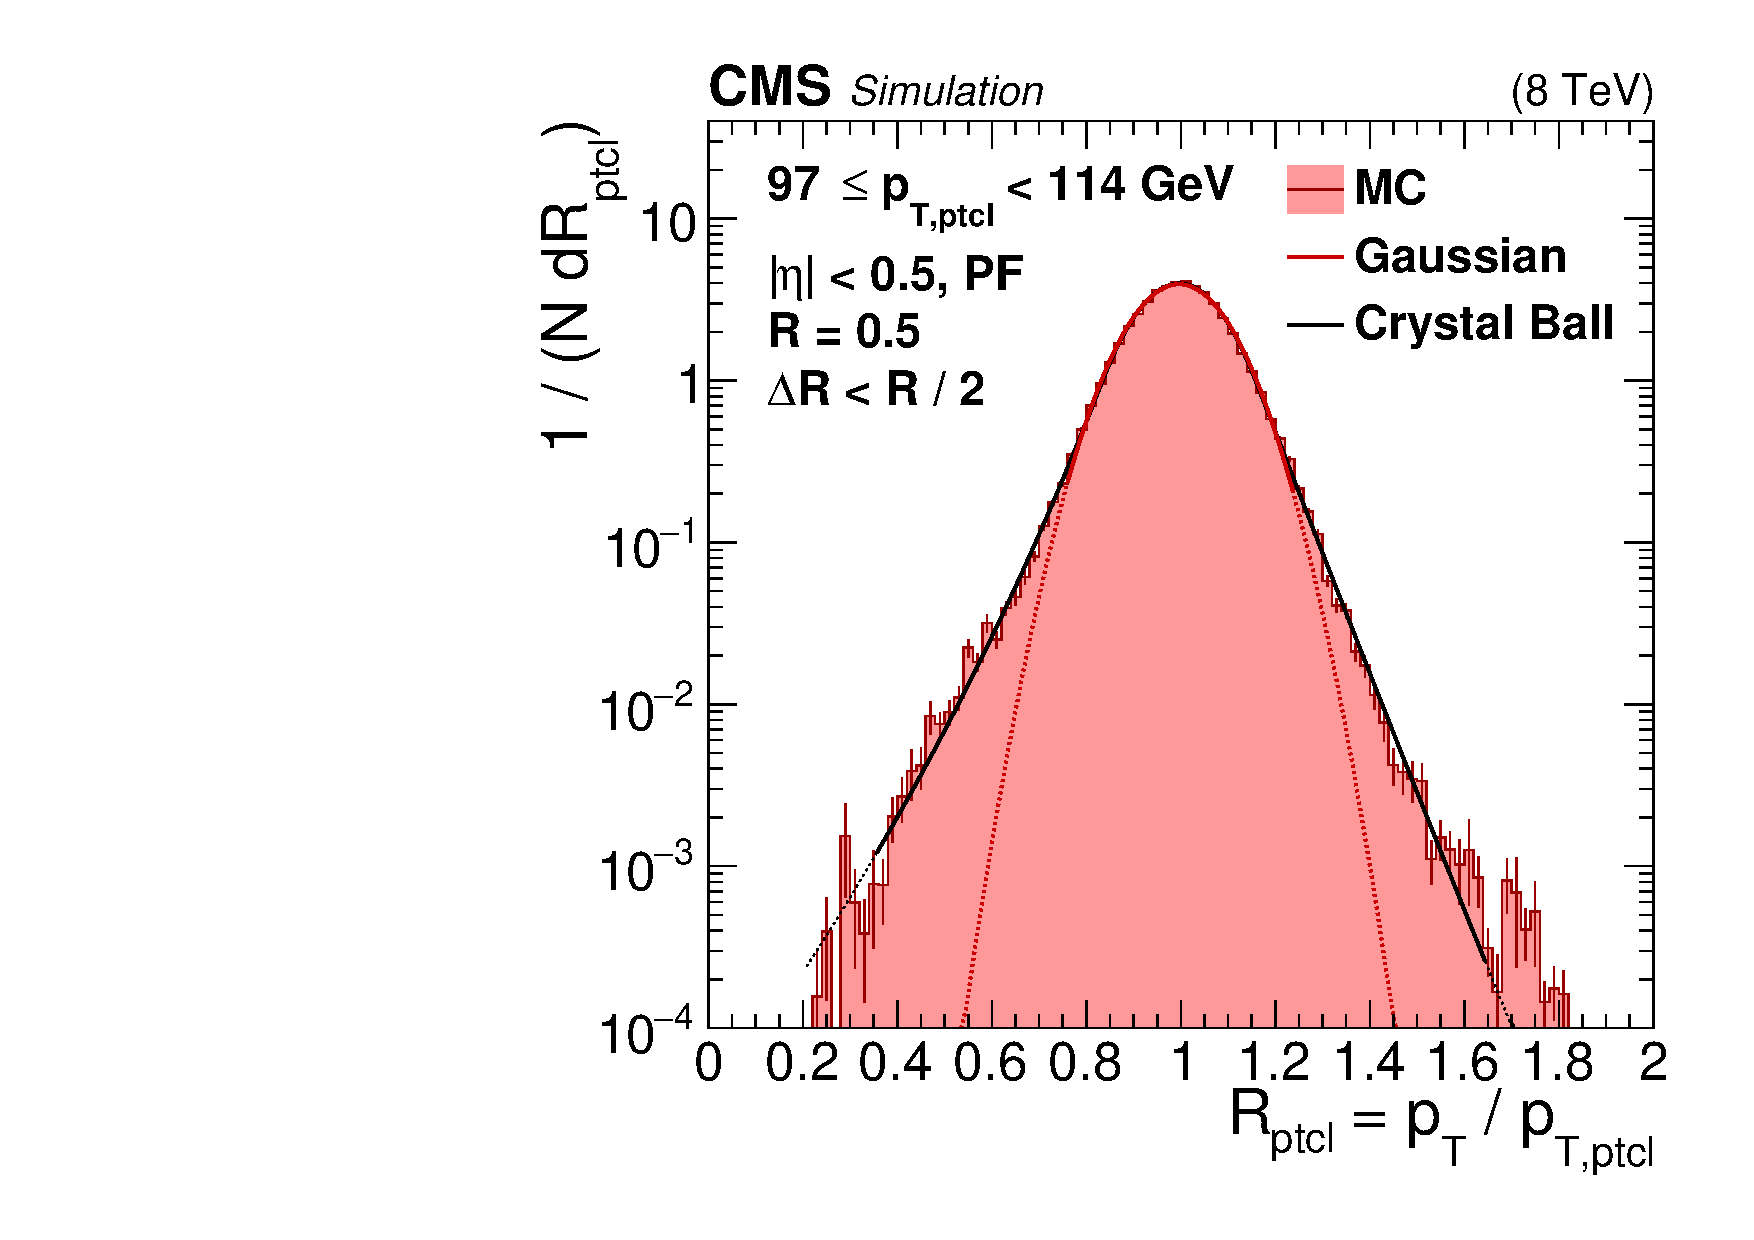
\includegraphics[width=0.85\textwidth]{figures/jet_resolution.pdf}
      \caption[Example plot of jet energy resolution template.]{
        $\mathrm{p}_{\mathrm{T,ptcl}}$ is the ``particle level'' \pt, the total energy that the jet's particle components actually had, while \pt is the energy measured by the detector.
        The horizontal axis is the ratio of these two quantities, and the vertical axis the probability that a jet's measured energy will differ from its true energy by that ratio.
        The response curve shown here applies to jets with particle level \pt in the band $97 < \pt < 114$~GeV, and measured in the CMS barrel.
        Large mismeasurements of jet energy are much less probable than small mismeasurements.
        The core is well-described by a Gaussian, but the tails are highly non-Gaussian and best described by a Crystal-Ball function.
        Taken from \cite{jet_resolution}.}
      \label{fig:jet_resolution}
    \end{figure}  


    Rebalance and Smear (R\&S) achieves the desired improvement.
    R\&S begins with a sample of multijet events from data with \Ht on the order of hundreds of GeV and at least two jets with $\pt > 10$~GeV.
    This is as nearly unbiased a sample of QCD events as is allowed by available triggers.
    These events will generically have some small but nonzero \met due to imperfect measurement of the jet energies, dictated by the detector's resolution, and potentially a very small contribution from genuine neutrinos produced in the hadron decay chains inside the jets.
    The \pt values assigned to the jets are then adjusted, finding the most likely assignment of \pt values subject to the hypothesis that the true \met is very nearly zero, and that jet mismeasurements of a given size occur with probability given by jet response templates.
    As shown in Figure~\ref{fig:jet_resolution}, large mismeasurements are rare.
    Thus, the Rebalancing step tries to get the \pt as close to zero as feasible without making more improbable adjustments to the jets than necessary.
    The output of the Rebalancing step is a large sample of real QCD events with maximally accurate jet \pt assignments.

    Then, each of these events goes through a Smearing step.
    This step randomly assigns a new \pt to each jet in the event according to the same jet response templates.
    The vast majority of the time, the new event looks as unremarkable as the original event before Rebalancing.
    Rarely, the output event passes the baseline selection and represents a potential mismeasurement event that might lie in the data signal region.
    The Smearing can be repeated as many times for each event as is desired, subject to computing limitations.
    The number of Smeared events falling into each signal region, from this sample of known equivalent integrated luminosity, can then be converted into the expected number of events that would fall into the signal region in data, due to jet mismeasurement.
    
  \begin{figure}[h!]
    \centering
    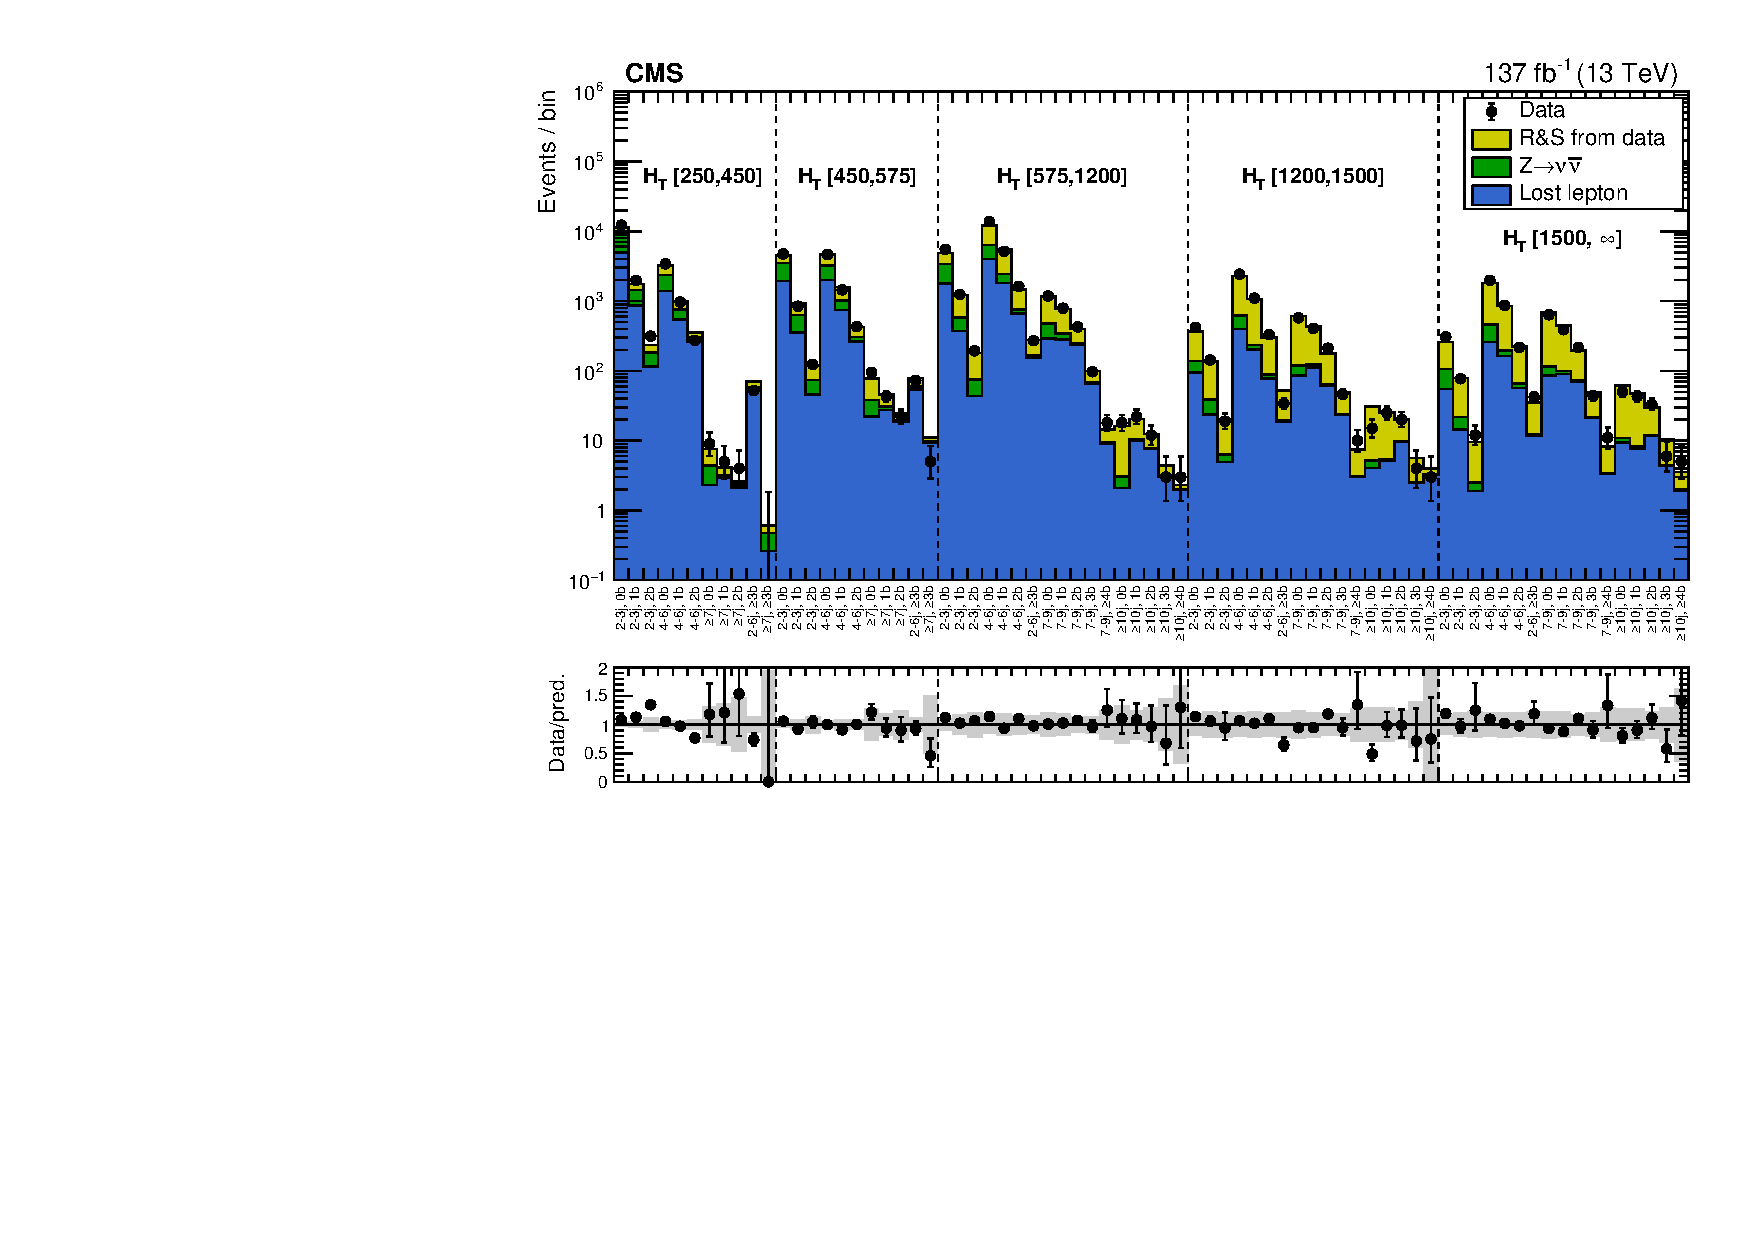
\includegraphics[width=0.85\textwidth]{figures/MT2_2019/Figure_003.pdf}
    \caption[Validation of the Rebalance and Smear jet mismeasurement background estimate in the $\dphimin < 0.3$ control region.]{
      The Rebalance and Smear jet mismeasurement background estimate is validated in the $\dphimin < 0.3$ control region. 
      The multijet mismeasurement event count predicted by Rebalance and Smear is shown in yellow, and contributes most of the event counts in this control region. 
      The combined background estimate (filled histogram) is consistent with the data observation (black data points).
      Taken from \cite{MT2_2019}.}
    \label{fig:RandSval}
  \end{figure}  

    Of course, many of the output events will have $\dphimin < 0.3$, falling outside of the signal region into the QCD-dominated low $\dphimin$ control region.
    This allows for a validation in data of the R\&S procedure, shown in Figure~\ref{fig:RandSval}.
    The total background estimate is consistent with data in the $\dphimin < 0.3$ control region across all of the analysis bins, with the R\&S estimated counts contributing most of the predicted events.

    R\&S achieves a significant improvement over the old $r_{\phi}$ based system, effectively eliminating statistical error, and improving the worst case relative error on the mismeasurement estimate from 180\% to less than 50\%.

    \subsubsection{Expanded Binning} \label{sec:newbinning}

    Although the baseline selection defines the class of events in which a signal of interest may be found, most signals will produce a significant number of events in only a subset of the phase space.
    For instance, a signal producing 4 top quarks in the final state (see Figure~\ref{fig:susyproduction} second row, right) will almost always produce events with $\njet \geq 7$, $\nb > 0$, and $\Ht \sim 1$~TeV.
    If the entire set of selected events is considered together, the entire background is combined, potentially hiding a signal.
    If instead the phase space is divided into many separate regions, the background in each region is smaller, so that the background count is as small as possible in the small subset of regions that any given signal actually populates.
    This sensitivity enhancement motivates very fine binning of the signal region.
    The classic search uses \mttwo, \Ht, \njet, and \nb as binning variables.

    In the 2016 version of the classic search \cite{MT2_2016}, the most extreme \njet\xspace bin was $\njet \geq 7$, and the most extreme \nb bin was $\nb \geq 3$.
    This limitation was imposed by limited statistics.
    The background estimate for each bin is performed separately, and the observed counts are subject to Poisson statistical flucuations.
    Binning too finely causes any potential sensitivity gains from better isolating signal to be lost to greater uncertainty in the expected background.
    The analysis binning was updated for the latest edition of the classic search \cite{MT2_2019}, anticipating the improved statistical power.
    The full set of new bins, along with the predicted background counts and observed event counts in data, is available in Appendix~\ref{app:classicbinning}.

    The new binning extends the old binning in three ways.
    First, new $\njet \geq 10$ bins were added to the $\Ht > 1200$~GeV regions.
    This allows for enhanced sensitivity to signals with extremely high jet multiplicity, such as the 4 top signal previously mentioned.
    Similarly, new $\nb \geq 4$ bins were added to these same regions, targeting the same signal.
    Sensitivity to some mass points of this signal model roughly doubled due to the addition of these bins, which have negligible background but appreciable signal counts.
    Finally, \mttwo binning was generally made narrower and the last bin moved to larger \mttwo values, for all signal regions, until the expected background in the last bin was on the order of 1 event.
    In all, there are 282 classic search bins, enhancing sensitivity to a broad array of potential signal models.

  \subsection{Signal Contamination} \label{sec:MT2sigcontam}

  The data driven estimate procedures for the neutrino backgrounds used control regions defined using leptons.
  Signals capable of producing leptons can contaminate these control regions, increasing the observed control region counts above the actual Standard Model production rate.
  This leads directly to an overprediction of background.
  For instance, consider stop pair production followed by decay to tops, as shown in Figure~\ref{fig:susyproduction} (row 3, right).
  Both tops will decay to a W and a bottom quark.
  If one of the W bosons decays leptonically and the lepton is reconstructed, the event will likely enter the single lepton control region.
  The lost lepton background, described in Section~\ref{sec:MT2lostlep}, will be overpredicted,
  \begin{equation}
    N_{LL}^{\mathrm{Data;Est}} = R_{MC}^{0\ell/1\ell} N_{SL}^{\mathrm{Data}} = R_{MC}^{0\ell/1\ell} \left(N_{SL}^{\mathrm{Data;SM}} + N_{SL}^{\mathrm{Data;BSM}}\right).
  \end{equation}
  The background overprediction is $\Delta N = R_{MC}^{0\ell/1\ell}N_{SL}^{\mathrm{Data;BSM}}$.
  For analysis purposes, the overprediction is modeled in simulation and treated as a reduction of the expected signal counts in every affected bin.
  \begin{equation}
    N_{SR}^{\mathrm{BSM;Adjusted}} = N_{SR}^{\mathrm{BSM;Raw}} - \Delta N
  \end{equation}
  This adjustment has the nice property that all terms are linear in the signal strength, so that it does not need to be recalculated for every signal strength considered when performing statistical analysis of the results.
  The same fraction of the signal is lost at every signal strength.
  
  As a result of this loss of sensitivity due to signal contamination, the classic analysis is less effective, all things equal, when used to search for signals that sometimes produce leptons than the naive expectation based on the leptonic versus hadronic branching ratios.
  This is an inevitable consequence of performing an all-hadronic search.

  \subsection{Results} \label{sec:MT2results}

  \begin{figure}[h!]
    \centering
    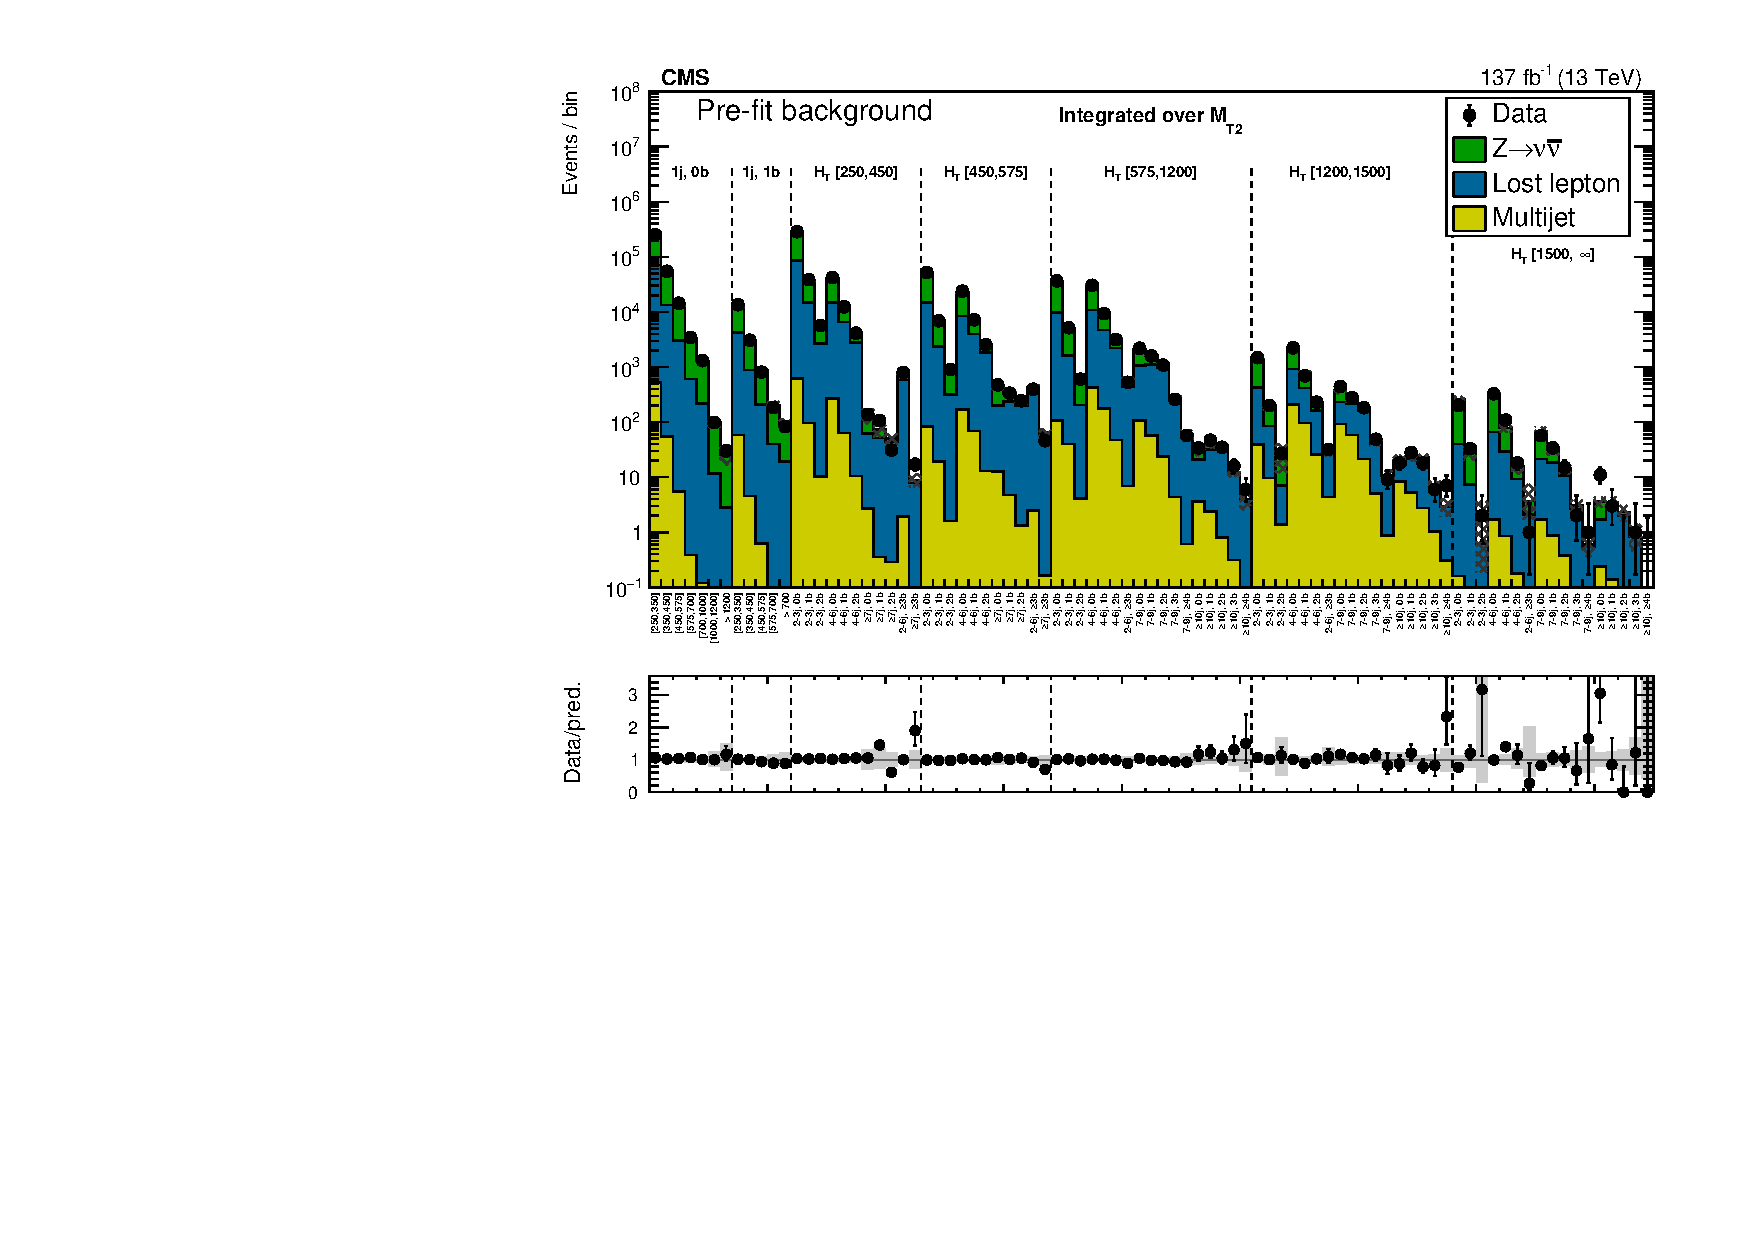
\includegraphics[width=0.85\textwidth]{figures/MT2_2019/Figure_005-a.pdf}
    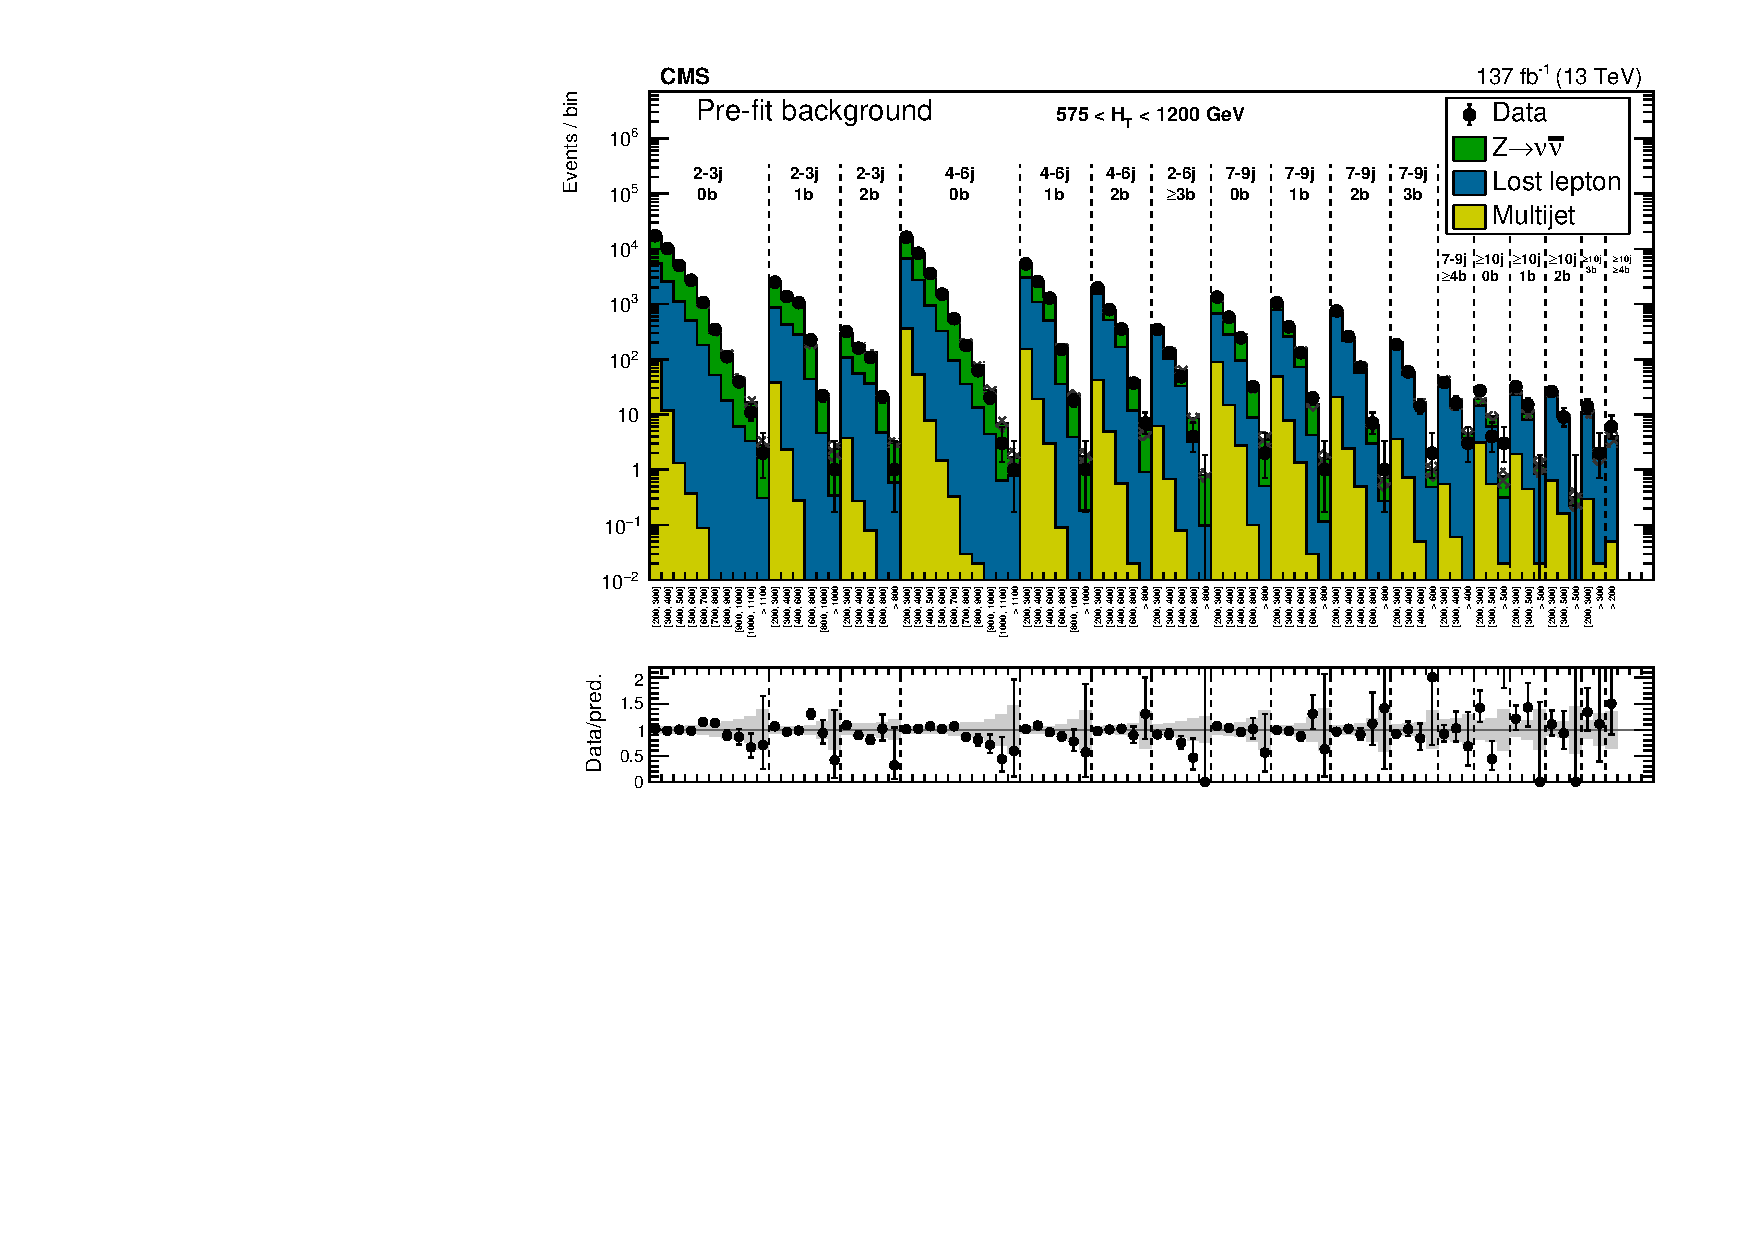
\includegraphics[width=0.85\textwidth]{figures/MT2_2019/Figure_005-b.pdf}
    \caption[Comparison of predicted background and observed data events in the classic search (upper) integrated over \Mttwo and (lower) for each of the medium \Ht search regions.]{Comparison of predicted background and observed data events in the classic search (upper) integrated over \Mttwo and (lower) for each of the medium \Ht search regions. Taken from \cite{MT2_2019}.}
    \label{fig:classicresults}
  \end{figure}  

  The full set of results for every classic search signal region, including every background prediction and the observed count, are available in Appendix~\ref{app:classicbinning}.
  The full set of results integrating over the \mttwo binning are display in Figure~\ref{fig:classicresults} (upper), and the results including the \mttwo binning for the $575 < \Ht < 1200$~GeV bins, the largest set, are shown in Figure~\ref{fig:classicresults} (lower).
  The observed counts are consistent with the background-only hypothesis, and the results are used to set exclusion limits at 95\% confidence level on the signals discussed in Section~\ref{sec:MT2sig}.

  \subsection{Limits} \label{sec:MT2limits}

  The statistical analysis procedure begins with maximum likelihood fits to the background-only and signal-plus-background hypotheses, for each signal model, considering each mass point separately. 
  The likelihoods are products of Poisson probabilities for each signal region bin, with log-normal constraint terms for each systematic affecting the predicted counts.
  Correlation between uncertainties affecting different bins are fully accounted for.
  As stated in the previous section, the background-only hypothesis is consistent with the observation.
  So, the parameter of interest for each signal model is the maximum signal cross section that can be excluded with 95\% confidence level.
  That is, the maximum possible production rate that the signal model could have, without requiring a combination of background and signal fluctuations more improbable than 1 in 20 to be consistent with the data.
  If the production cross section excluded at 95\% CL is less than the theoretical cross section for a given signal model, that signal model is said to be excluded at 95\% CL.

  The simplified supersymmetric extensions to the Standard Model shown in Figure~\ref{fig:susyproduction} have only two free parameters, the masses of the pair-produced superpartner, and the mass of the lightest supersymmetric particle, the dark matter candidate \lsp.
  Plotting the gluino or squark mass on the horizontal axis and the mass of \lsp on the vertical axis, then marking the mass points excluded at exactly 95\% CL, produces the exclusion curves shown in Figures~\ref{fig:t5x}--\ref{fig:stop_other}.
  Points to the lower left of these curves are excluded, while points above and to the right are not, as they require fluctuations no more improbable than 1 in 20 to be consistent with present data.

  The CMS dataset was collected only once, and this dataset is subject to fluctuations.
  The multiple exclusion curves shown on each plot, some in red and some in black, provide an indication of how unusual the limits generated by this dataset were.
  Suppose that the background's expected event count in a given region, summing across this entire dataset, is $B$.
  It is clearly possible that the actual number of background events that occur in the dataset in this bin could be around $B+\sqrt{B}$, or $B-\sqrt{B}$.
  In the first case, the analysis will draw unexpectedly strong limits on signals that populate this bin.
  In the second case, the analysis will draw unexpectedly weak limits on signals.

  The curves shown in red are the median, 1 standard deviation, and 2 standard deviation expected exclusion curves, in the background-only hypothesis.
  Together, these indicate the typical range of exclusion curves across many imaginary CMS datasets in which there is no signal to find.
  The curves in black are those that were observed in the CMS dataset as actually recorded.
  When the black observed curves extend out beyond the red expected curves, the analysis likely benefitted from a downward fluctuation of background.
  In cases where the observed curves swing inward compared to the expected curves, the analysis may have experienced an analogous unlucky upward fluctuation of background that mimicked a small signal, or alternatively there may be a genuine small signal lurking in the data that is resisting exclusion!

  The general shape of the curves is set by a combination of the falling cross section with increasing gluino or squark mass shown in Figure~\ref{fig:SUSYxsec}, and a loss of signal efficiency and signal versus background discriminatory power when the mass splitting between the gluino or squark and \lsp is small.
  On the lower right hand side of the plots lie signals that produce spectacular, energetic events, but at a very low rate due to the large mass of the gluino and squark, and accordingly small pair-production cross section.
  Moving up along the \lsp mass axis towards the upper right, the events remain spectacular, so the exclusion curves remain roughly vertical, limited only by the production cross section.
  Eventually, the mass splitting becomes small enough that the loss of signal efficiency and signal versus background discriminatory power becomes significant, and the exclusion curve turns to the left, towards lower mass squarks or gluinos and higher production rates.
  Decreasing the gluino or squark mass at fixed \lsp mass reduces the mass splitting, so the curve generally must also drop down somewhat along the \lsp mass axis to maintain a reasonable splitting.
  Eventually, the curve intercepts the $M_{\lsp} = M_{\tilde{g}}$ or $M_{\lsp} = M_{\tilde{q}}$ line.
  At this mass and below, all points are excluded even in the limit of zero mass splitting.


\begin{figure*}[htbp]
  \centering
    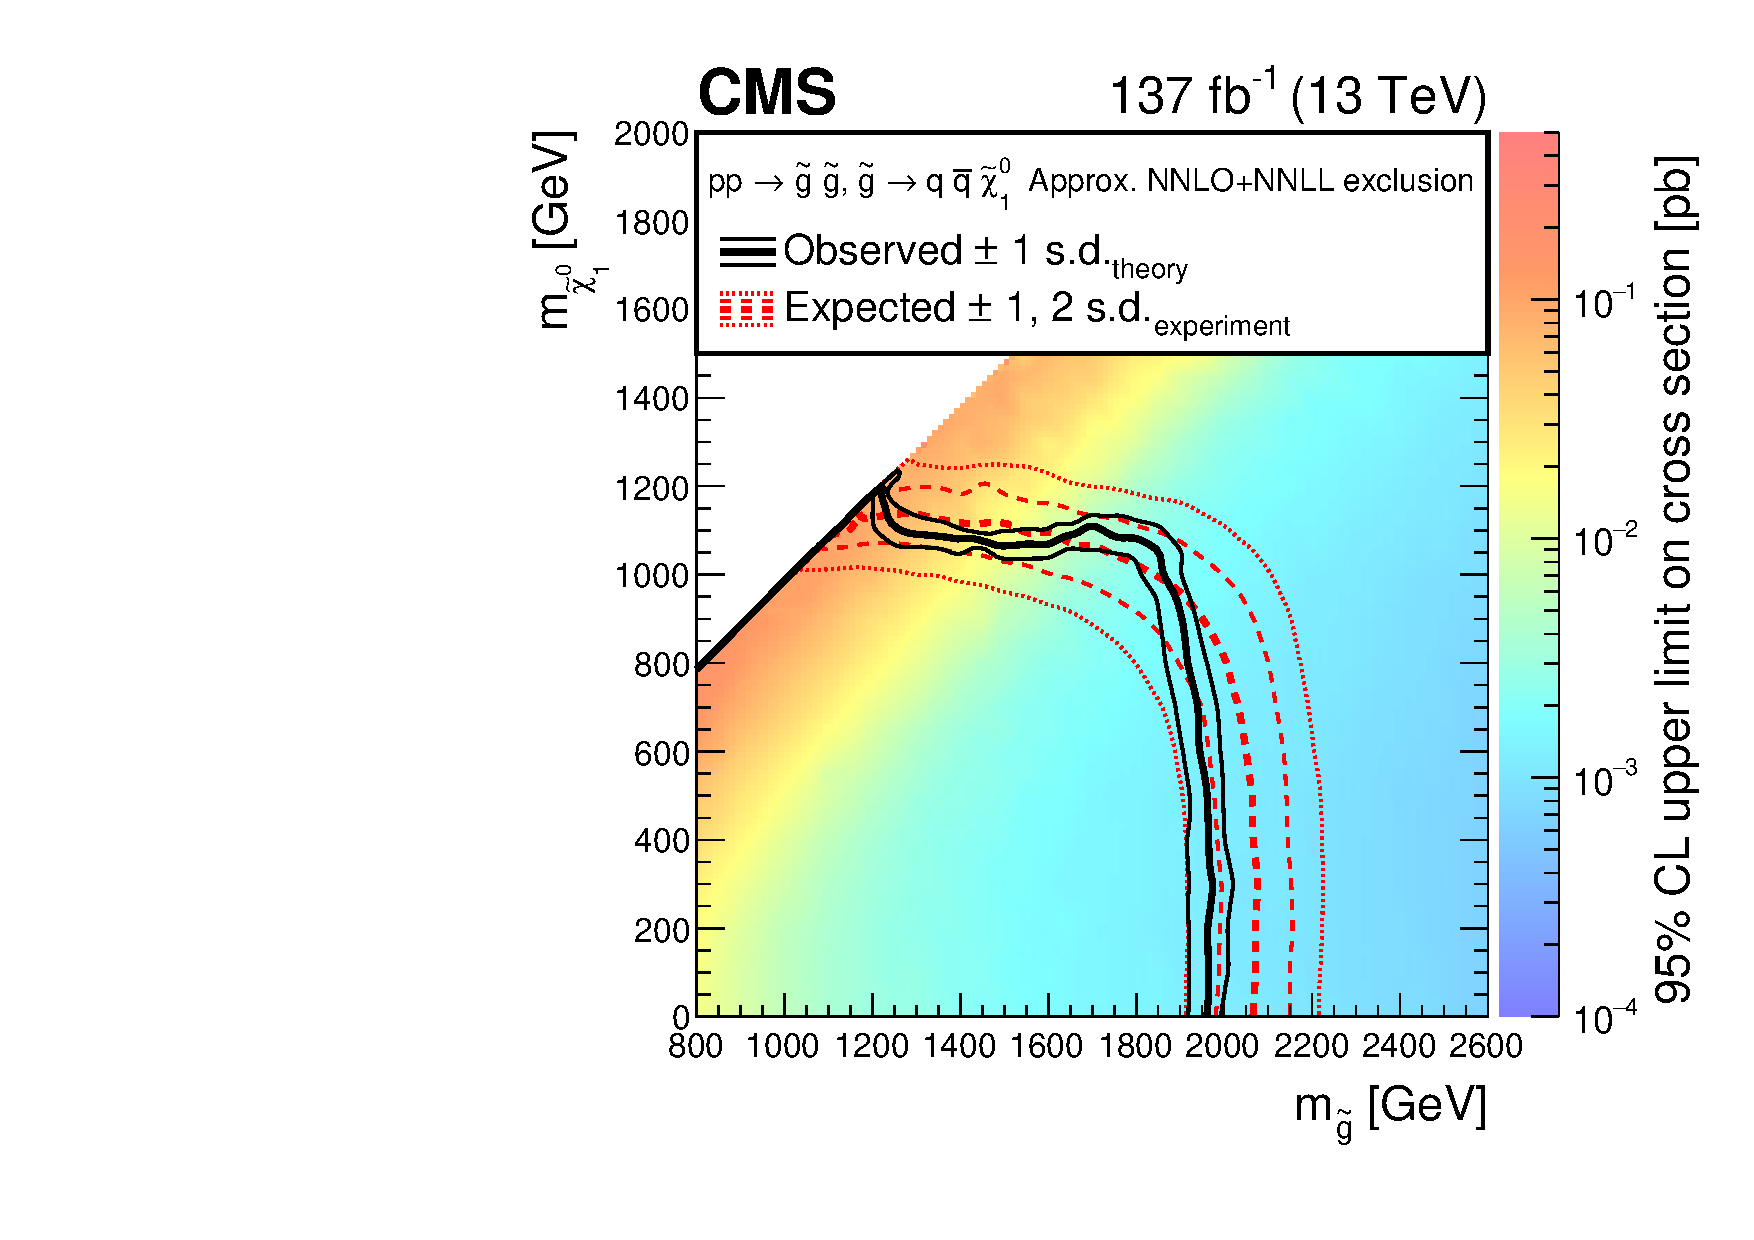
\includegraphics[width=0.48\textwidth]{figures/MT2_2019/Figure_011-a}\\
    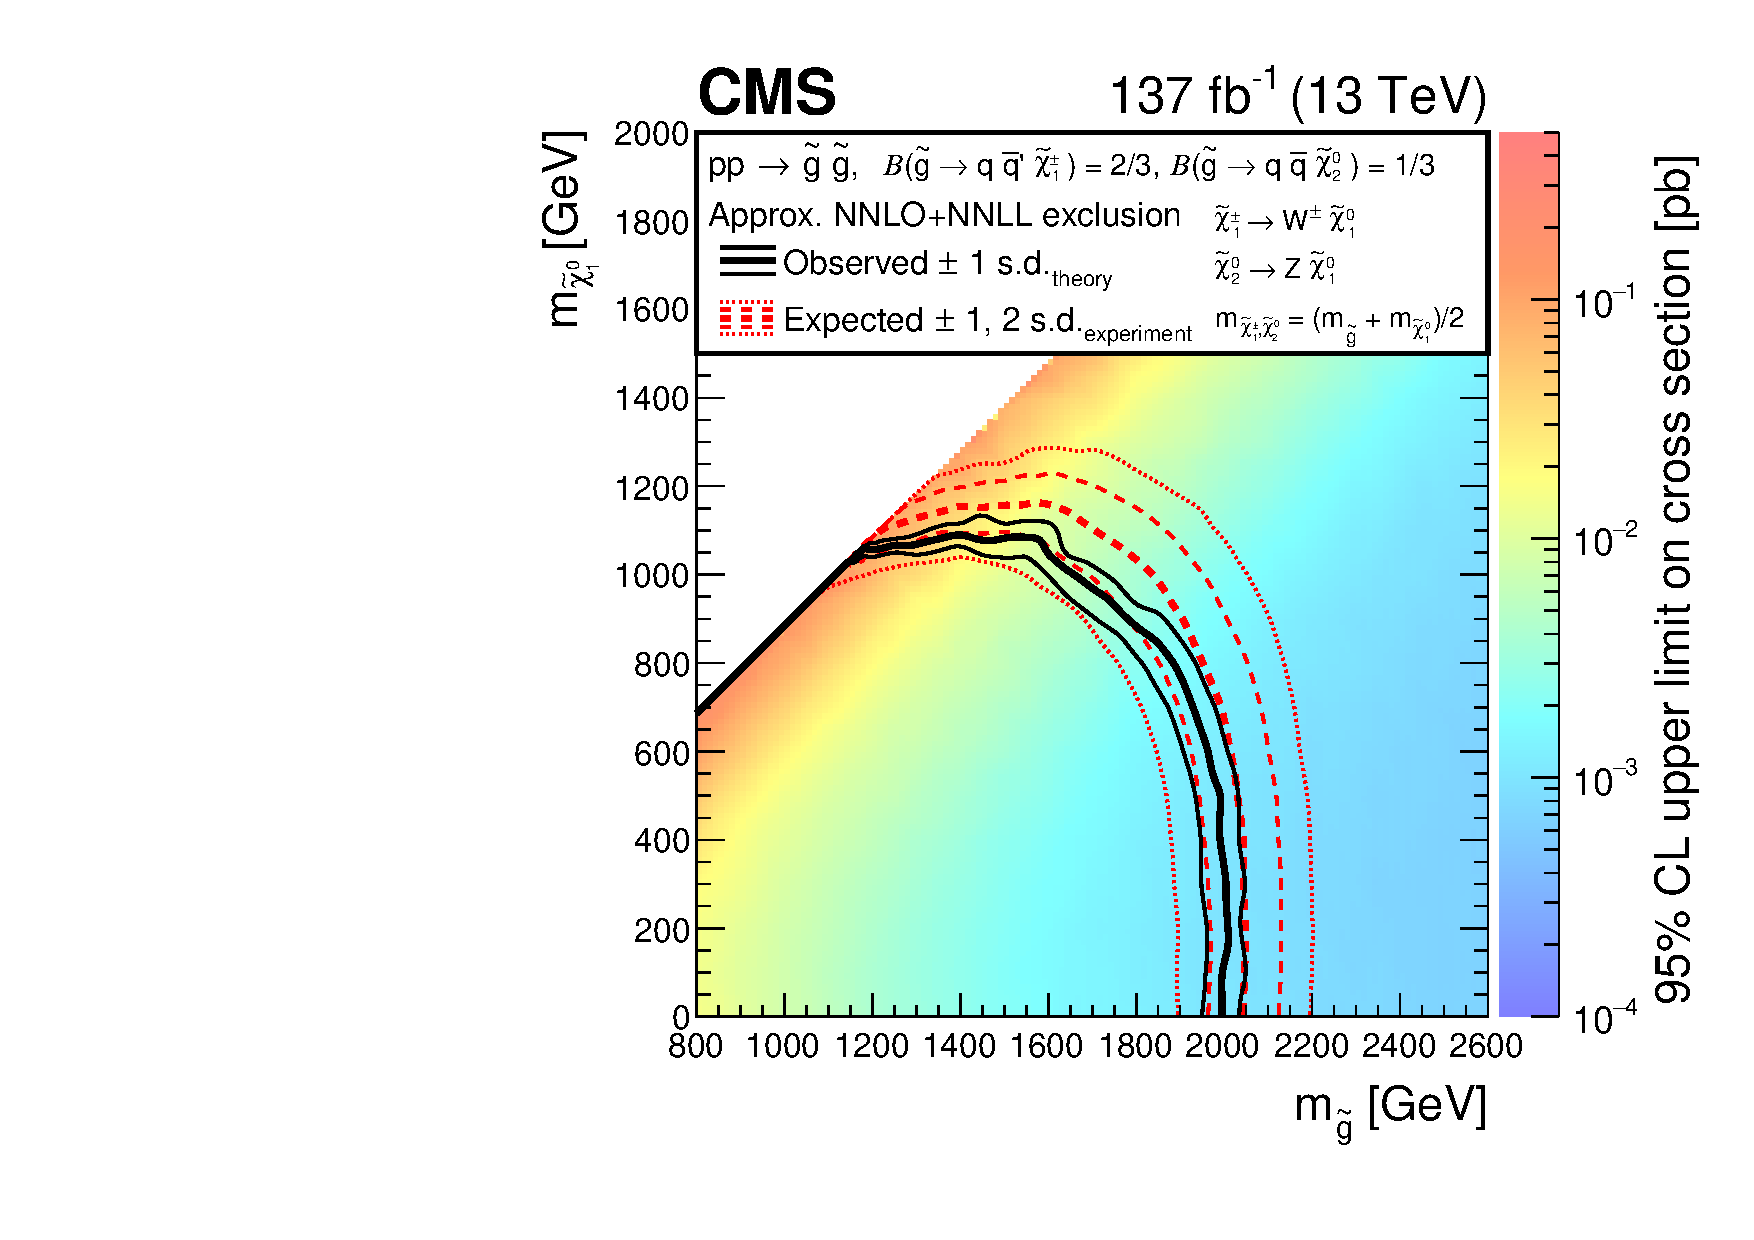
\includegraphics[width=0.48\textwidth]{figures/MT2_2019/Figure_011-b}
    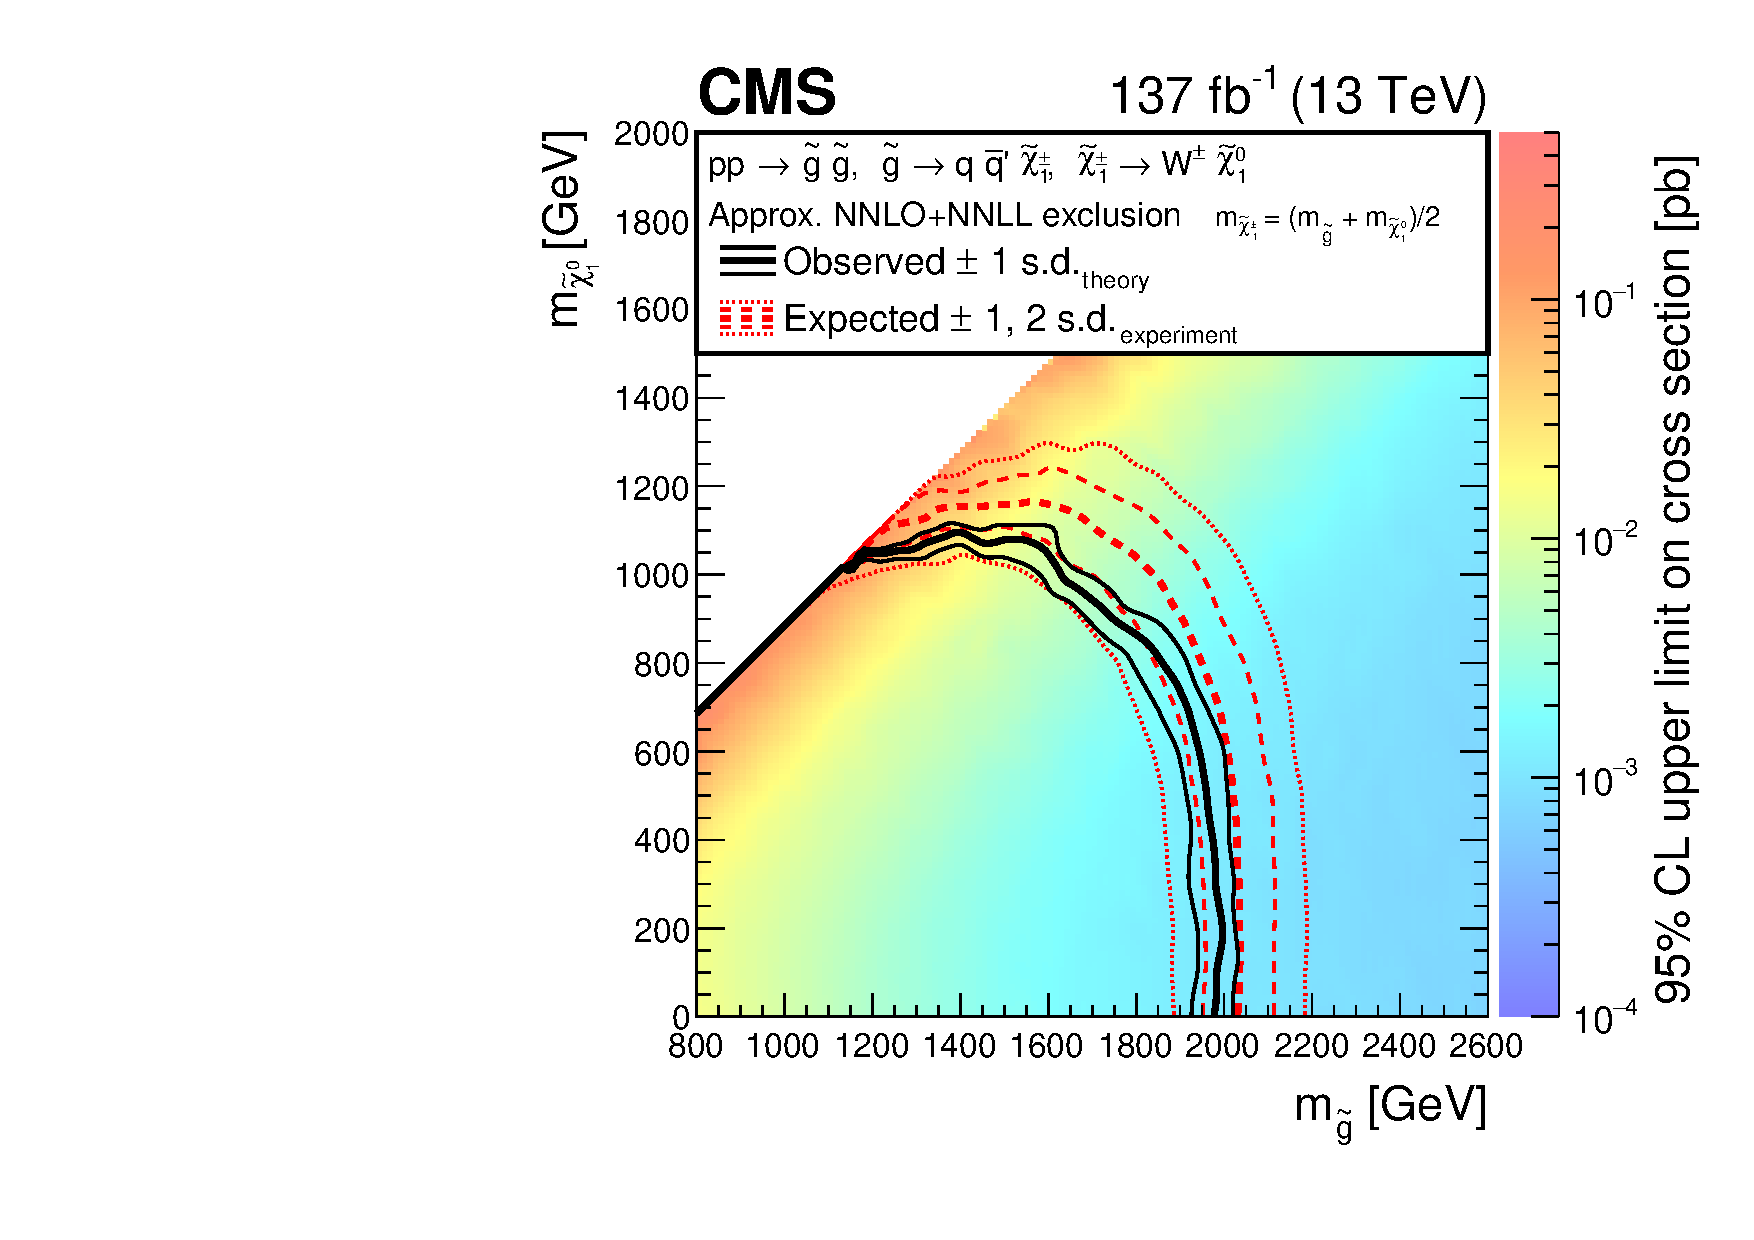
\includegraphics[width=0.48\textwidth]{figures/MT2_2019/Figure_011-c}
    \caption[Exclusion limits for gluino pair production and decay to light quarks.]{Exclusion limits at 95\% \CL for gluino pair production and decay to a pair of light quark jets and (upper) \lsp, (lower left) a democratic split between \lsp, \chitwo, which then decays to a Z boson and \lsp, and \chargino, which decays to a W boson and \lsp, and (lower right) \chargino then W and \lsp with 100\% branching fraction. Taken from \cite{MT2_2019}.}
    \label{fig:t5x}
\end{figure*}

\begin{figure*}[htbp]
  \centering
    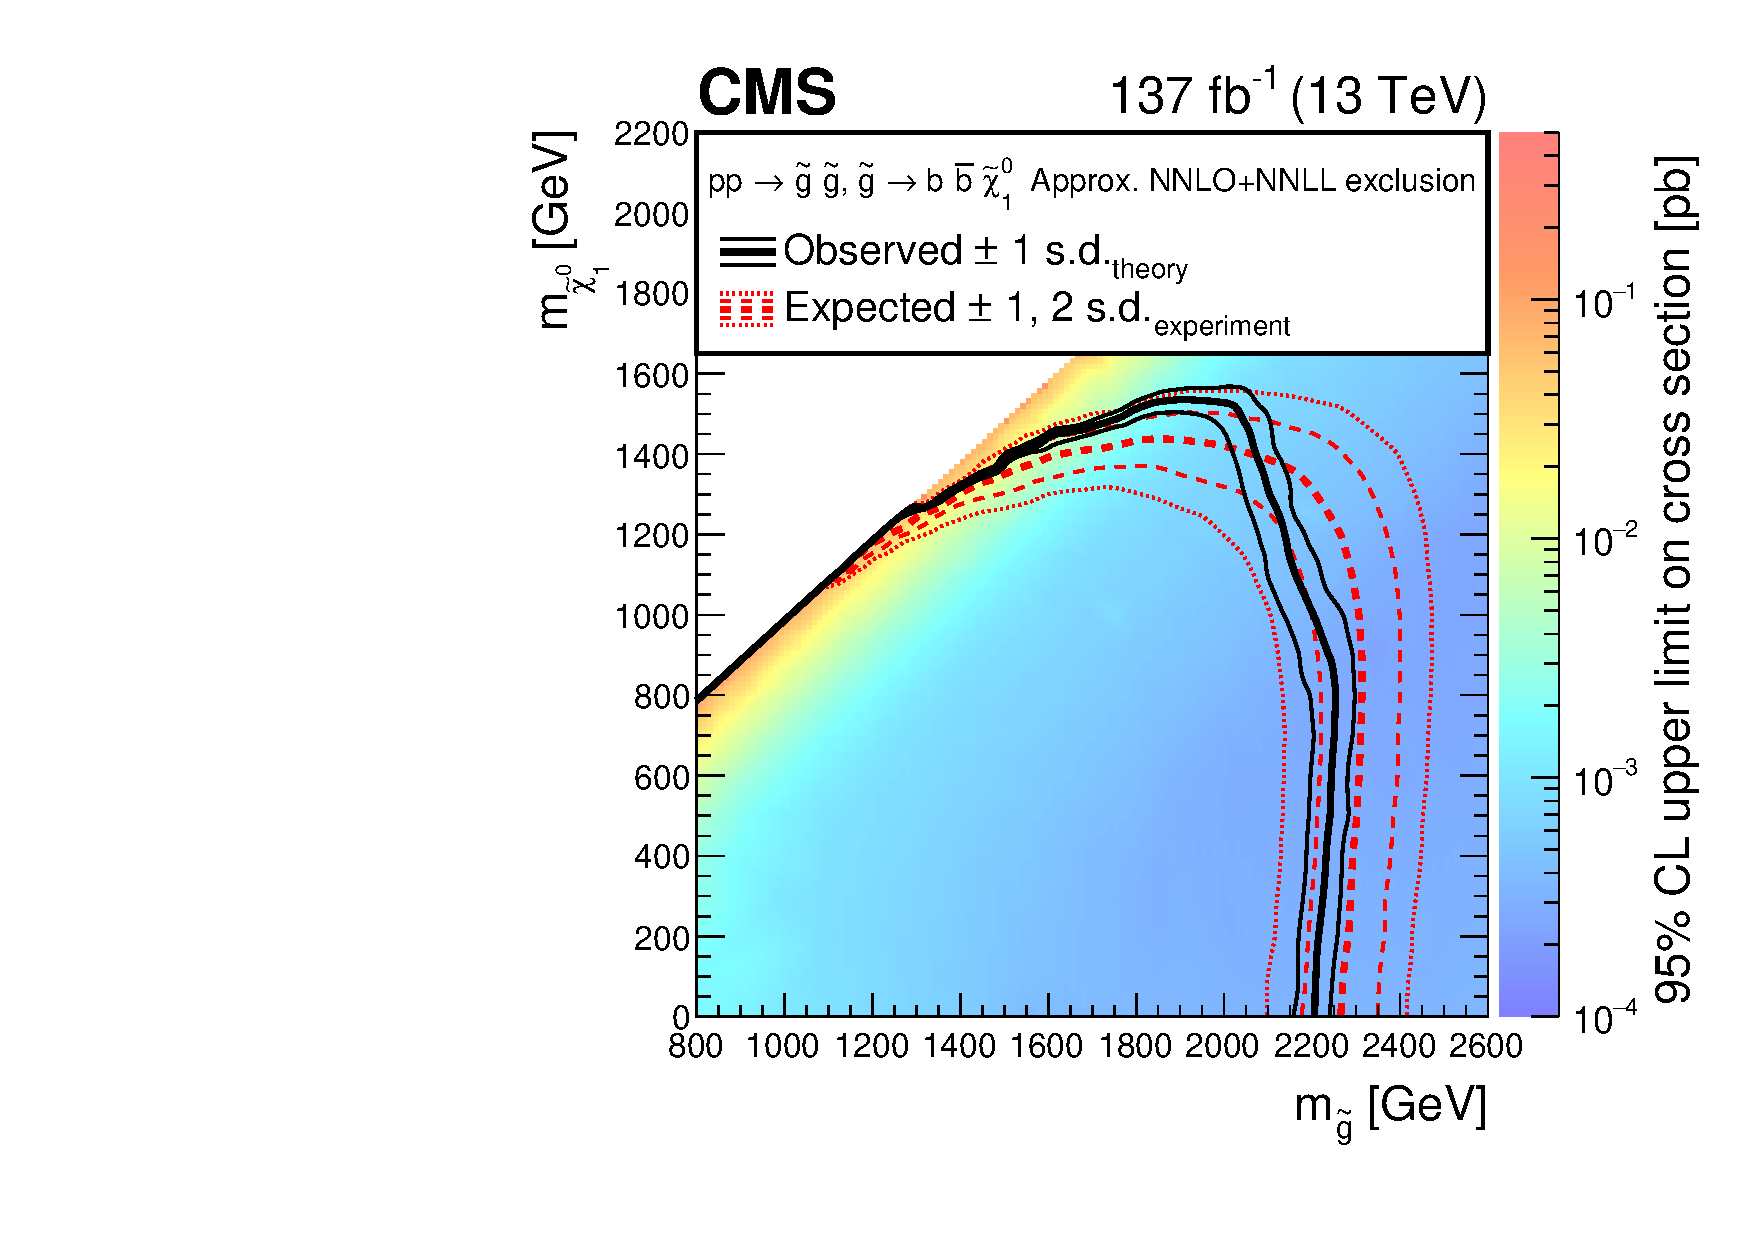
\includegraphics[width=0.48\textwidth]{figures/MT2_2019/Figure_012-a}
    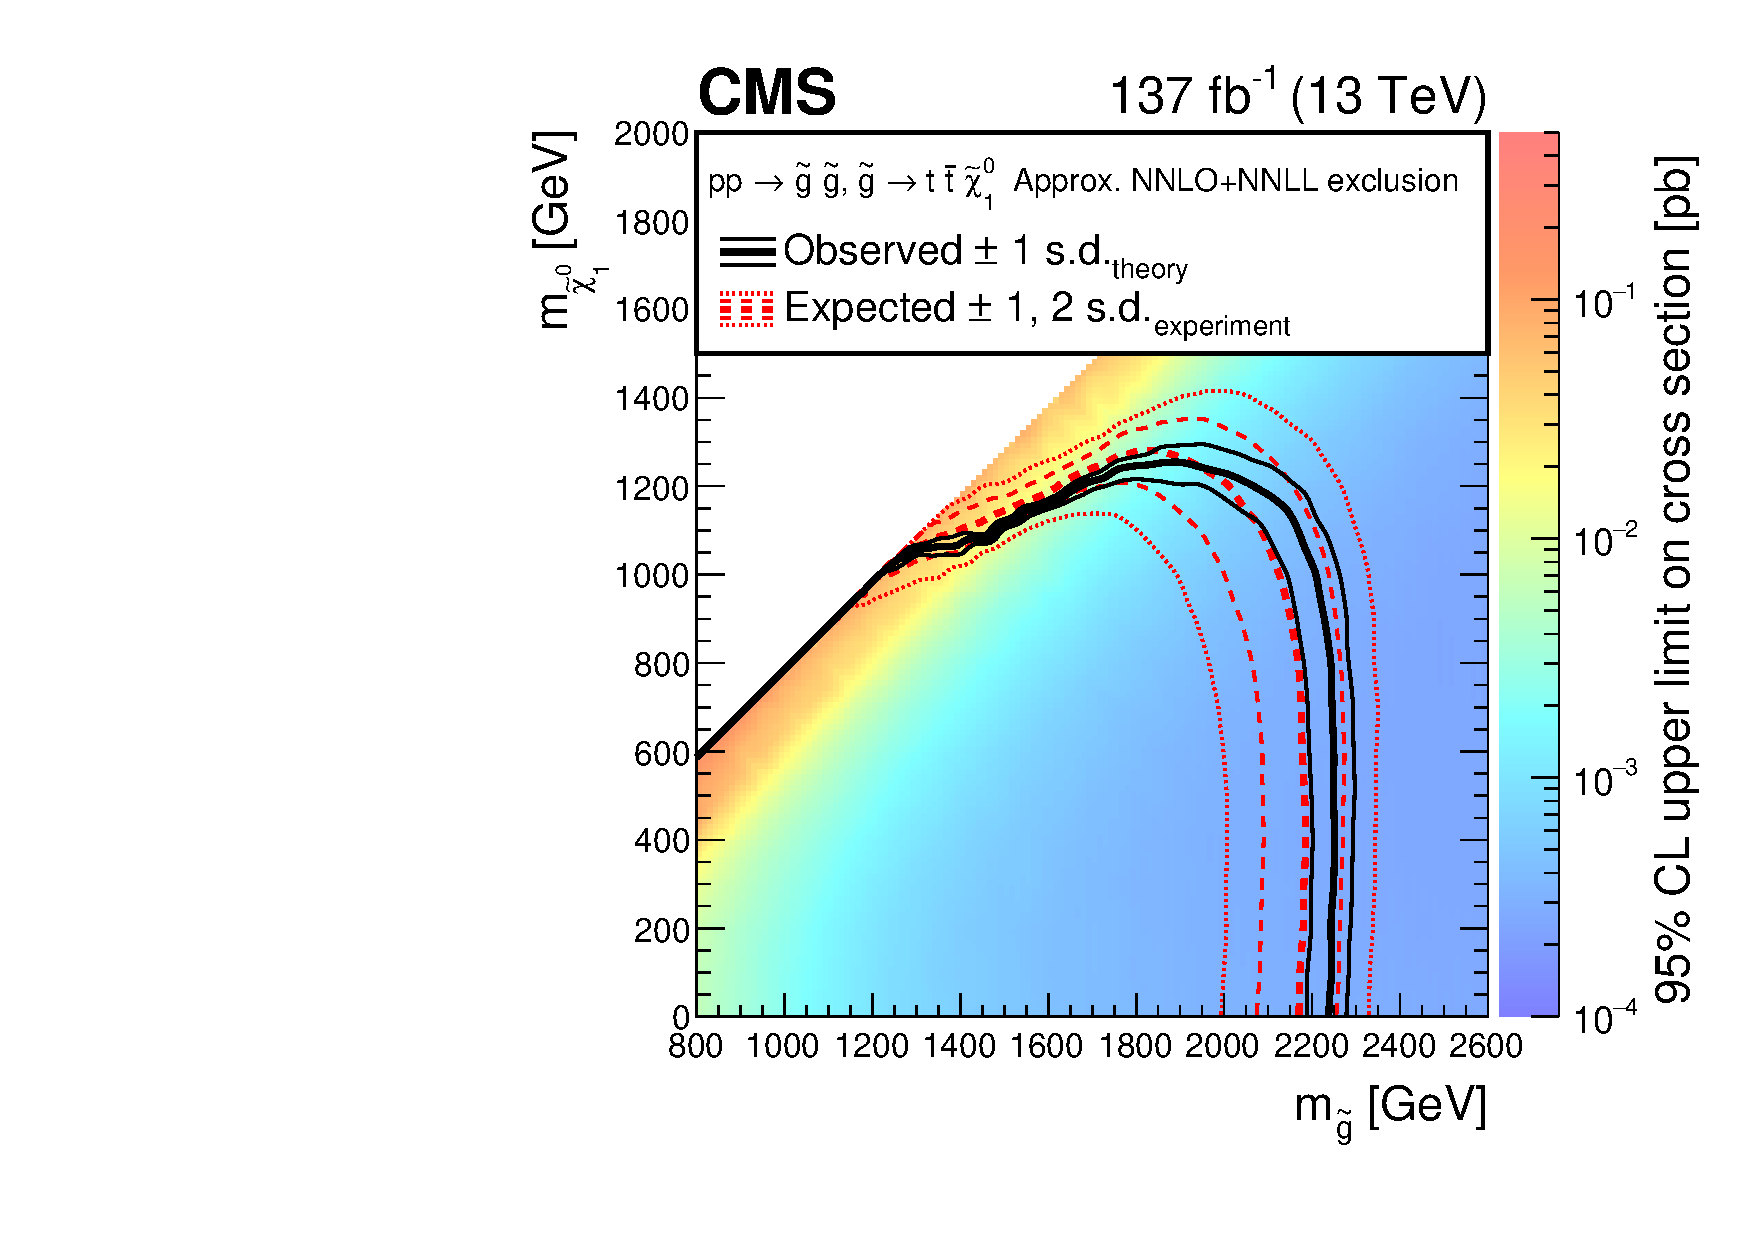
\includegraphics[width=0.48\textwidth]{figures/MT2_2019/Figure_012-b}
    \caption[Exclusion limits for gluino pair production and decay to bottom (left) and top (right) quarks.]{Exclusion limits at 95\% \CL for gluino pair production and decay to (left) bottom quarks and (right) top quarks. Taken from \cite{MT2_2019}.}
    \label{fig:t1x}
\end{figure*}

\begin{figure*}[htbp!]
  \centering
    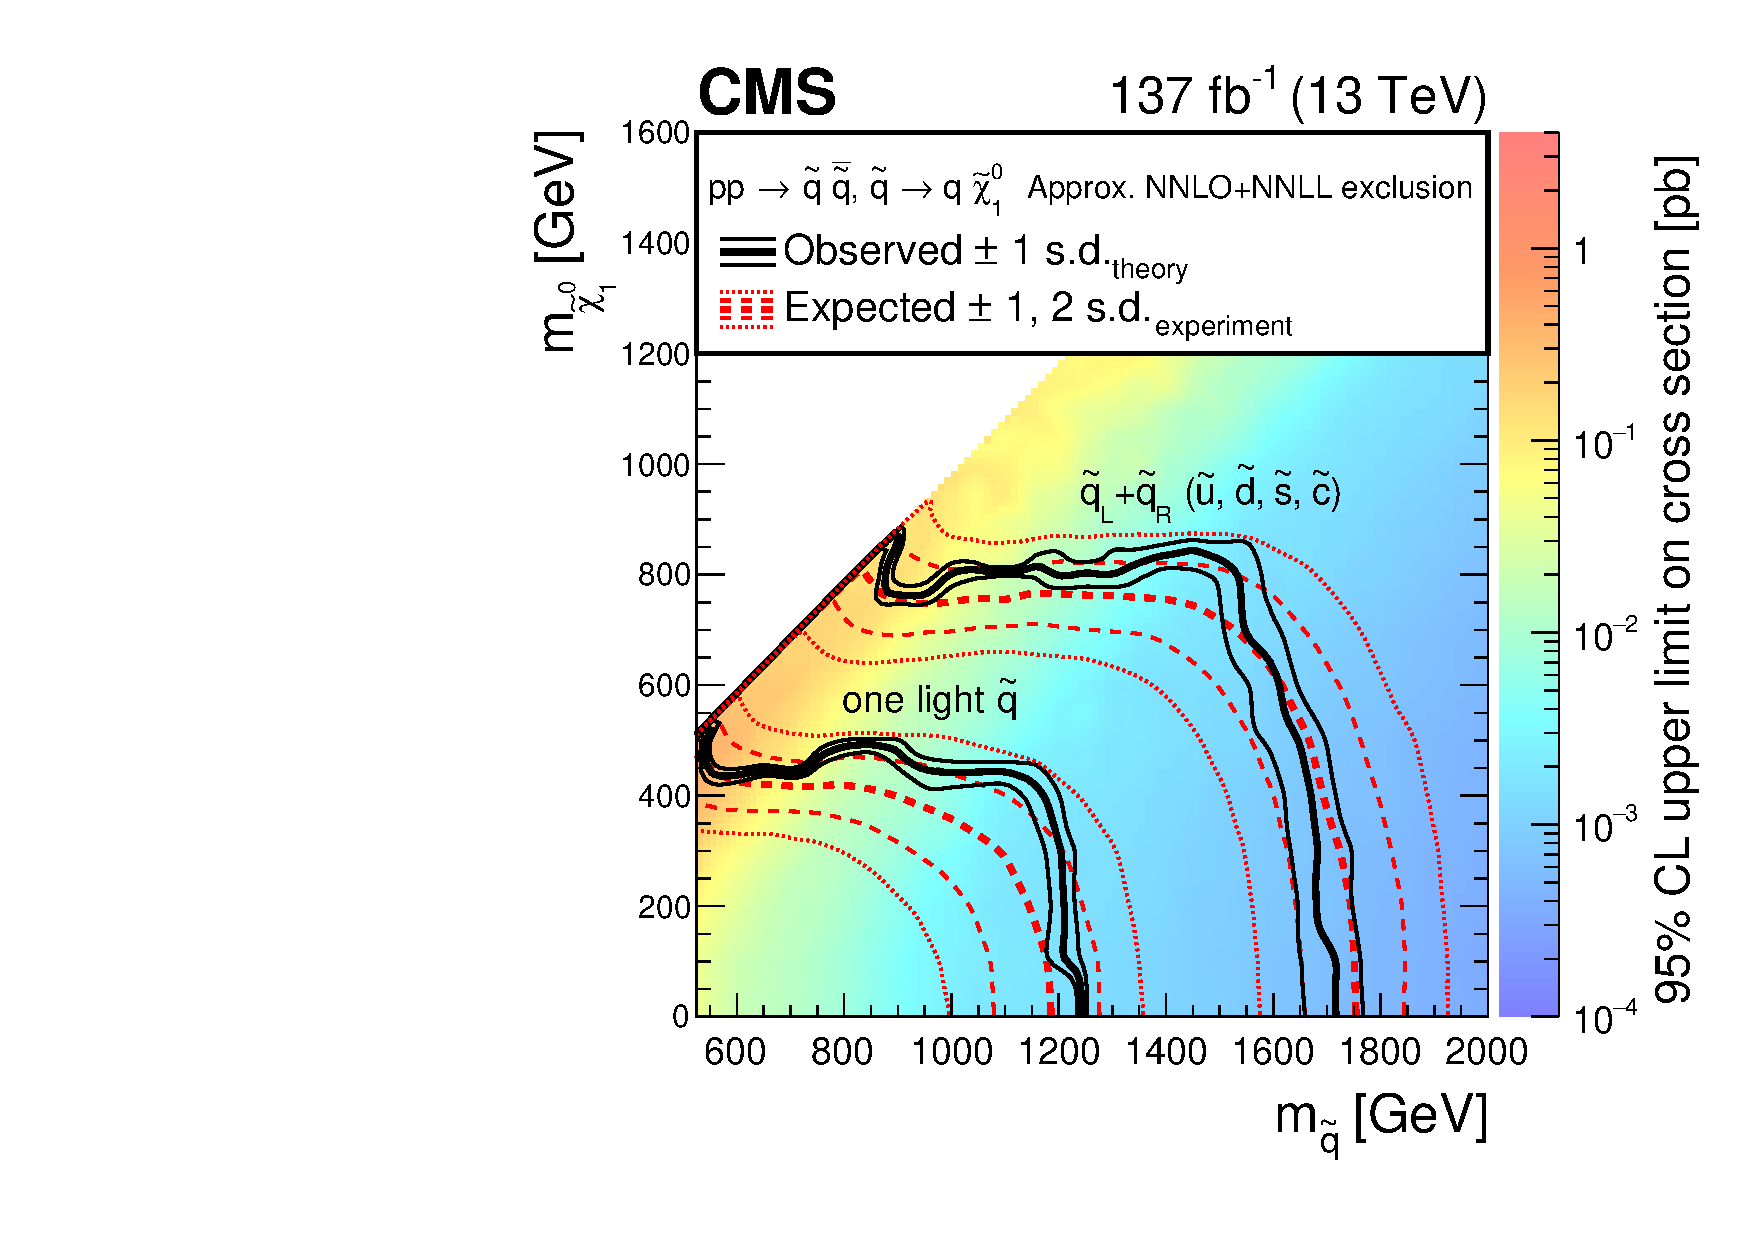
\includegraphics[width=0.48\textwidth]{figures/MT2_2019/Figure_013-a}
    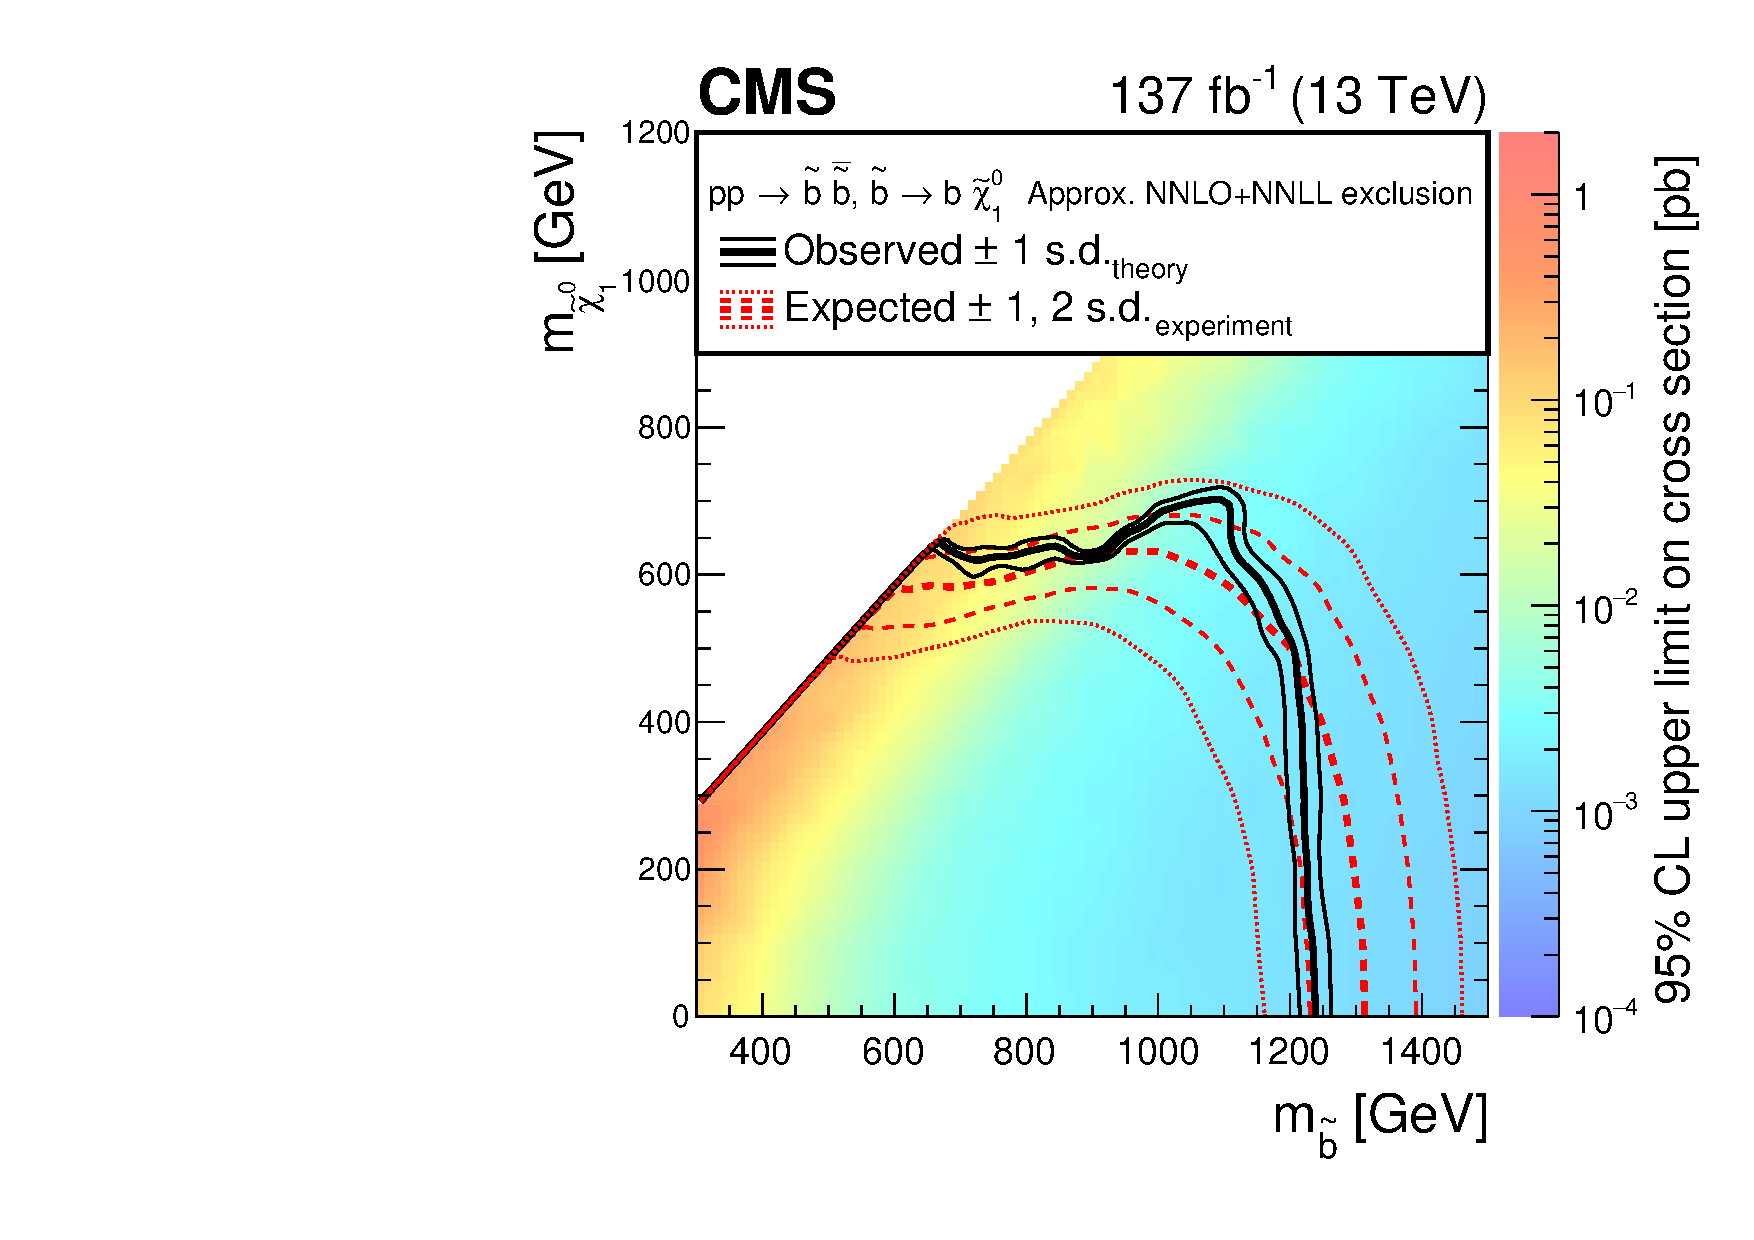
\includegraphics[width=0.48\textwidth]{figures/MT2_2019/Figure_013-b}
    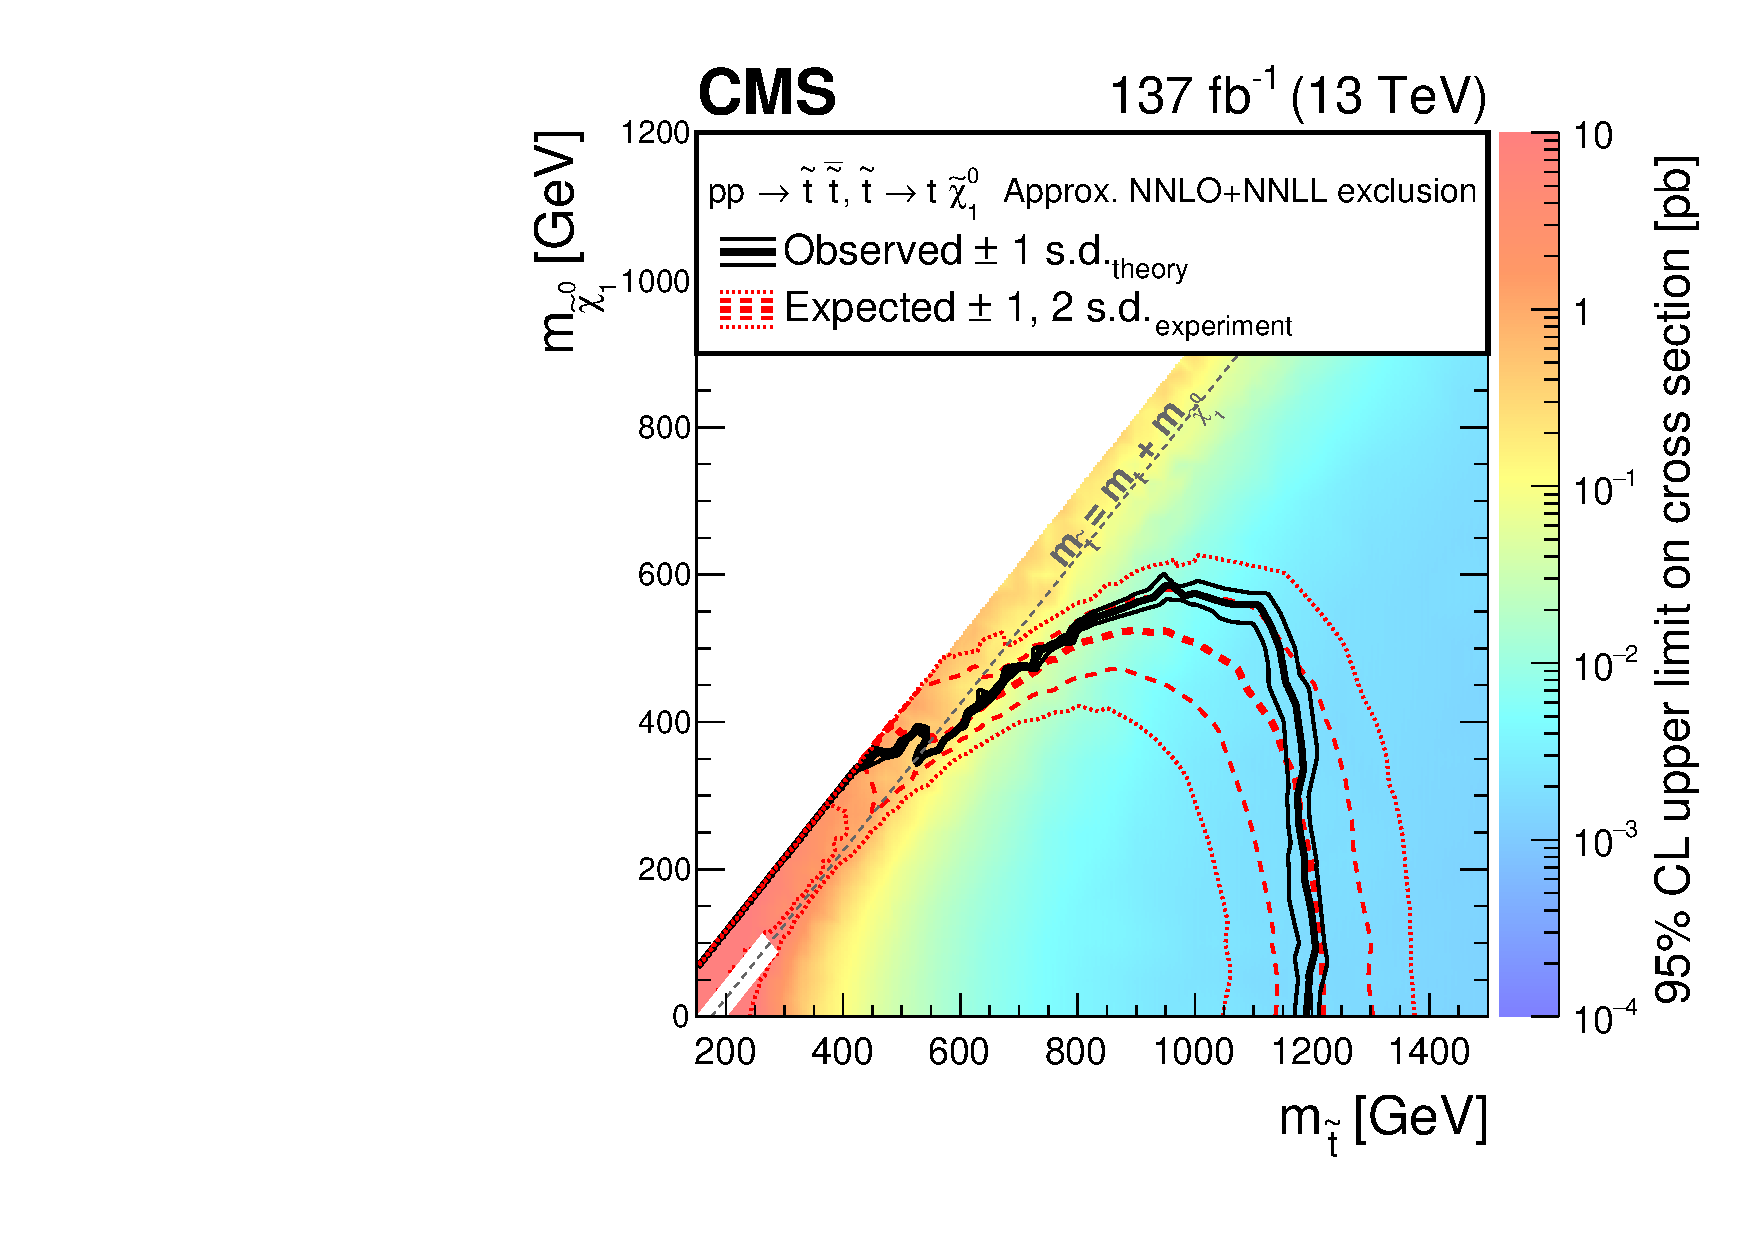
\includegraphics[width=0.48\textwidth]{figures/MT2_2019/Figure_013-c}
    \caption[Exclusion limit at 95\% \CL for (upper left) light-flavor squark pair production, (upper right) bottom squark pair production,
    and (lower) top squark pair production.]{Exclusion limit at 95\% \CL for (upper left) light-flavor squark pair production, (upper right) bottom squark pair production,
    and (lower) top squark pair production. Taken from \cite{MT2_2019}.}
    \label{fig:t2x}
\end{figure*}

\begin{figure*}[htbp!]
 \centering
   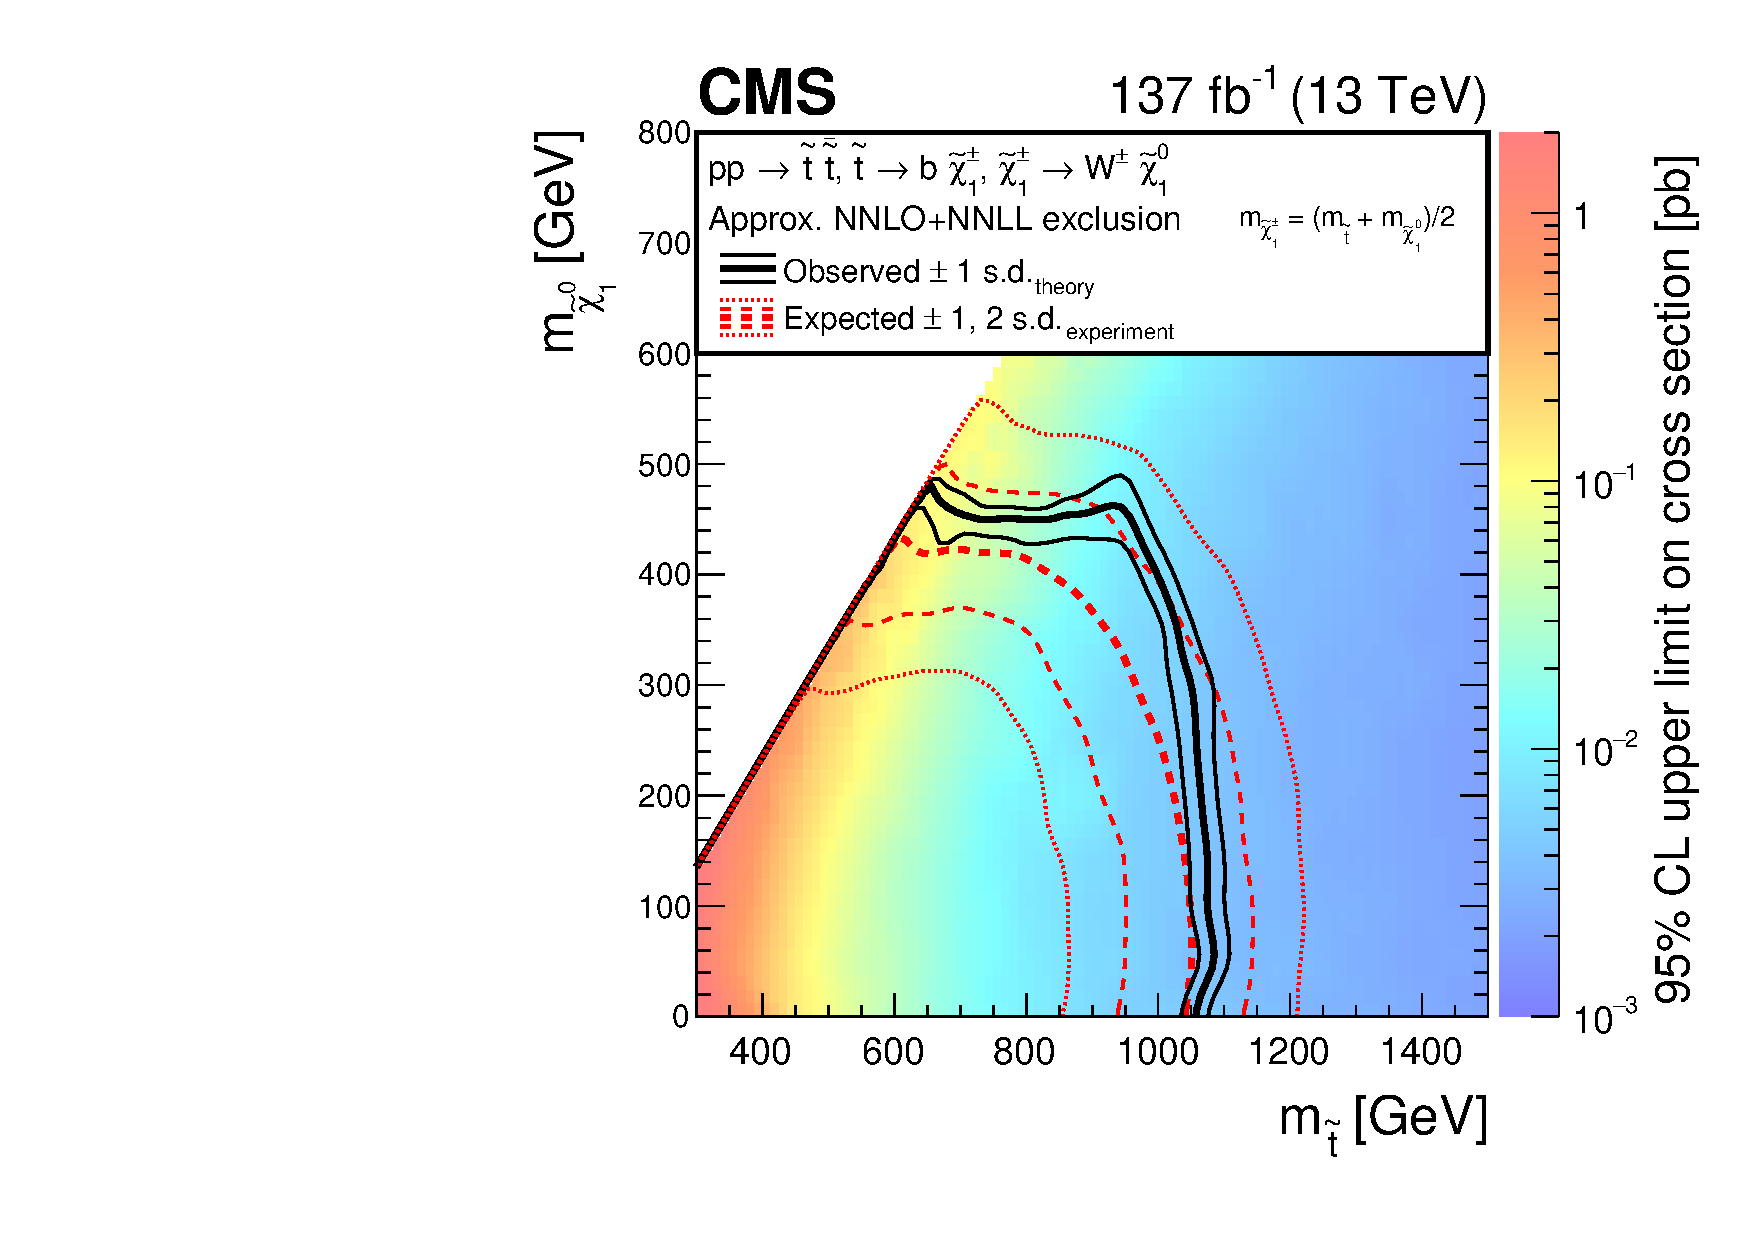
\includegraphics[width=0.49\textwidth]{figures/MT2_2019/Figure_014-a}
   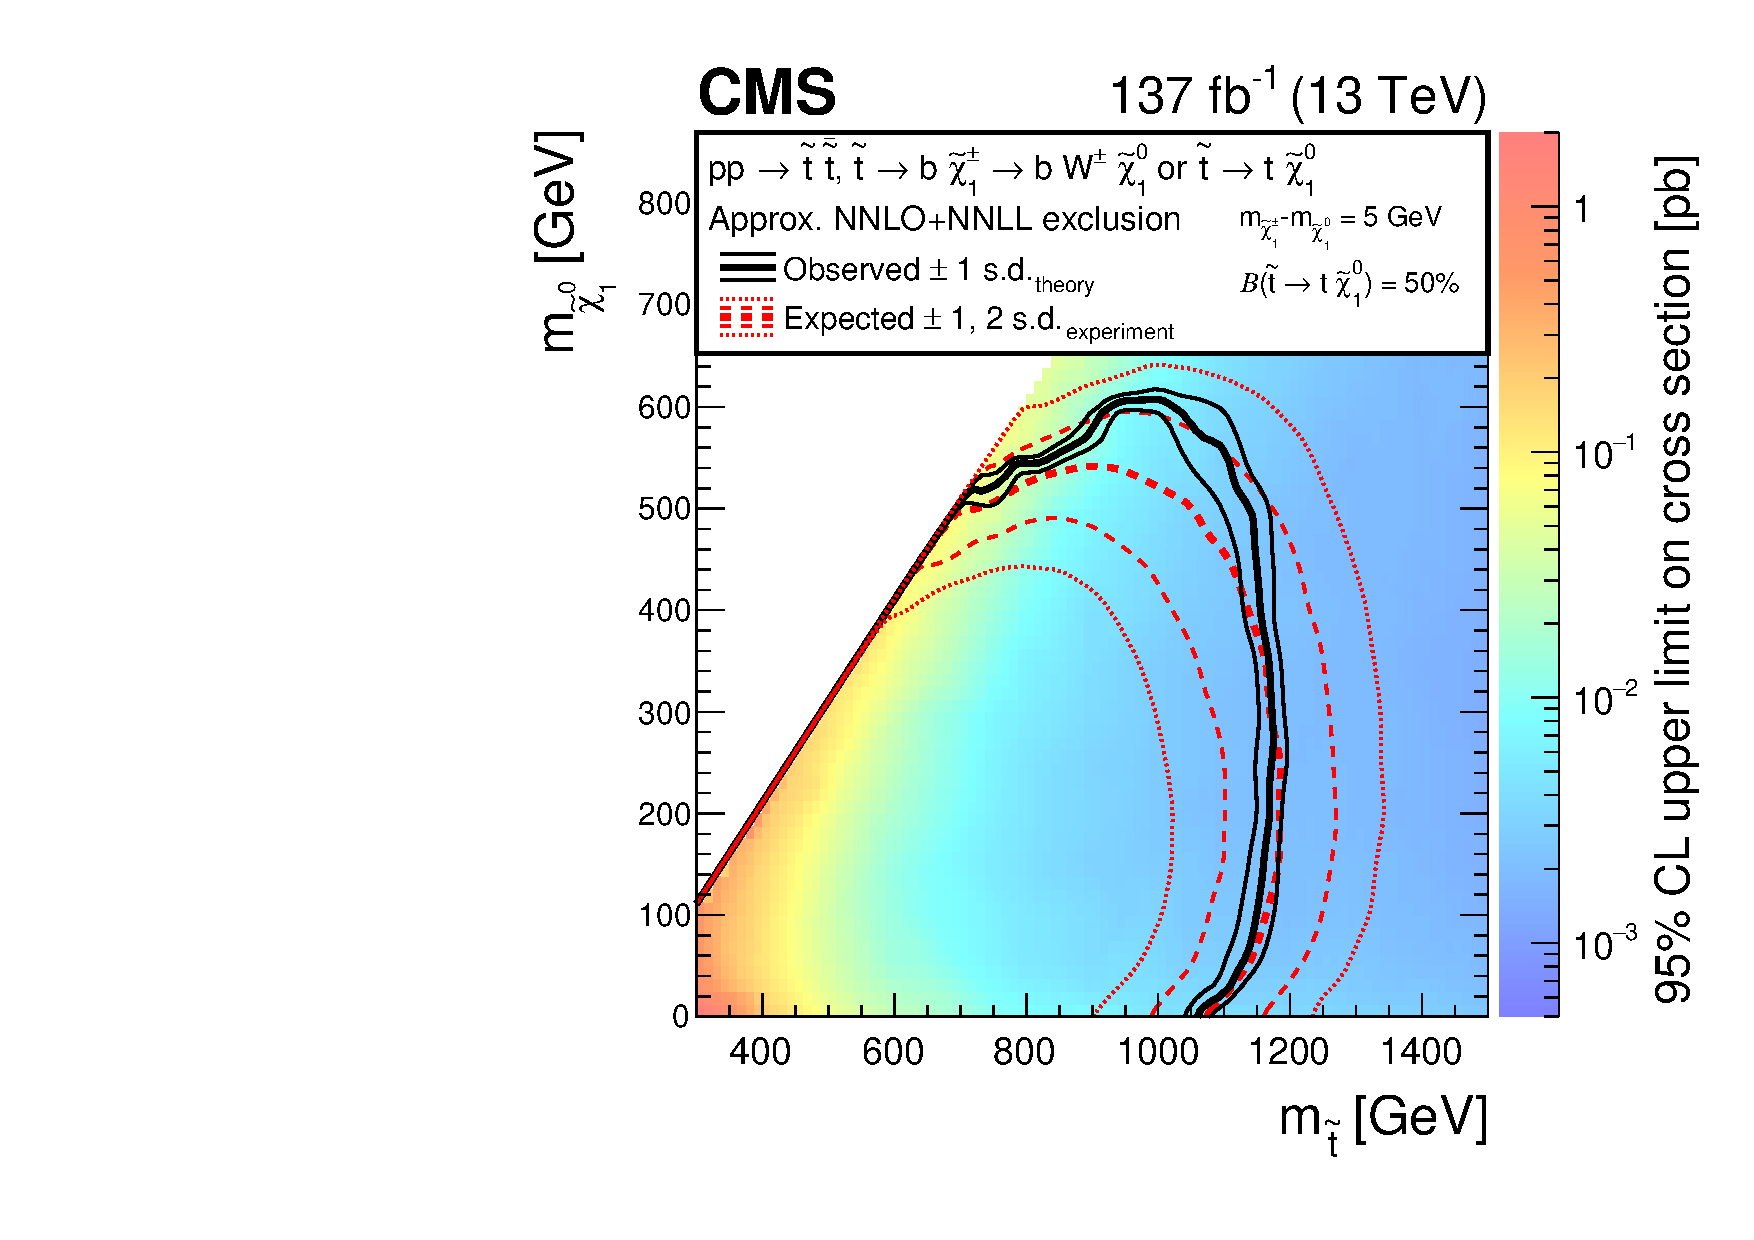
\includegraphics[width=0.49\textwidth]{figures/MT2_2019/Figure_014-b}
   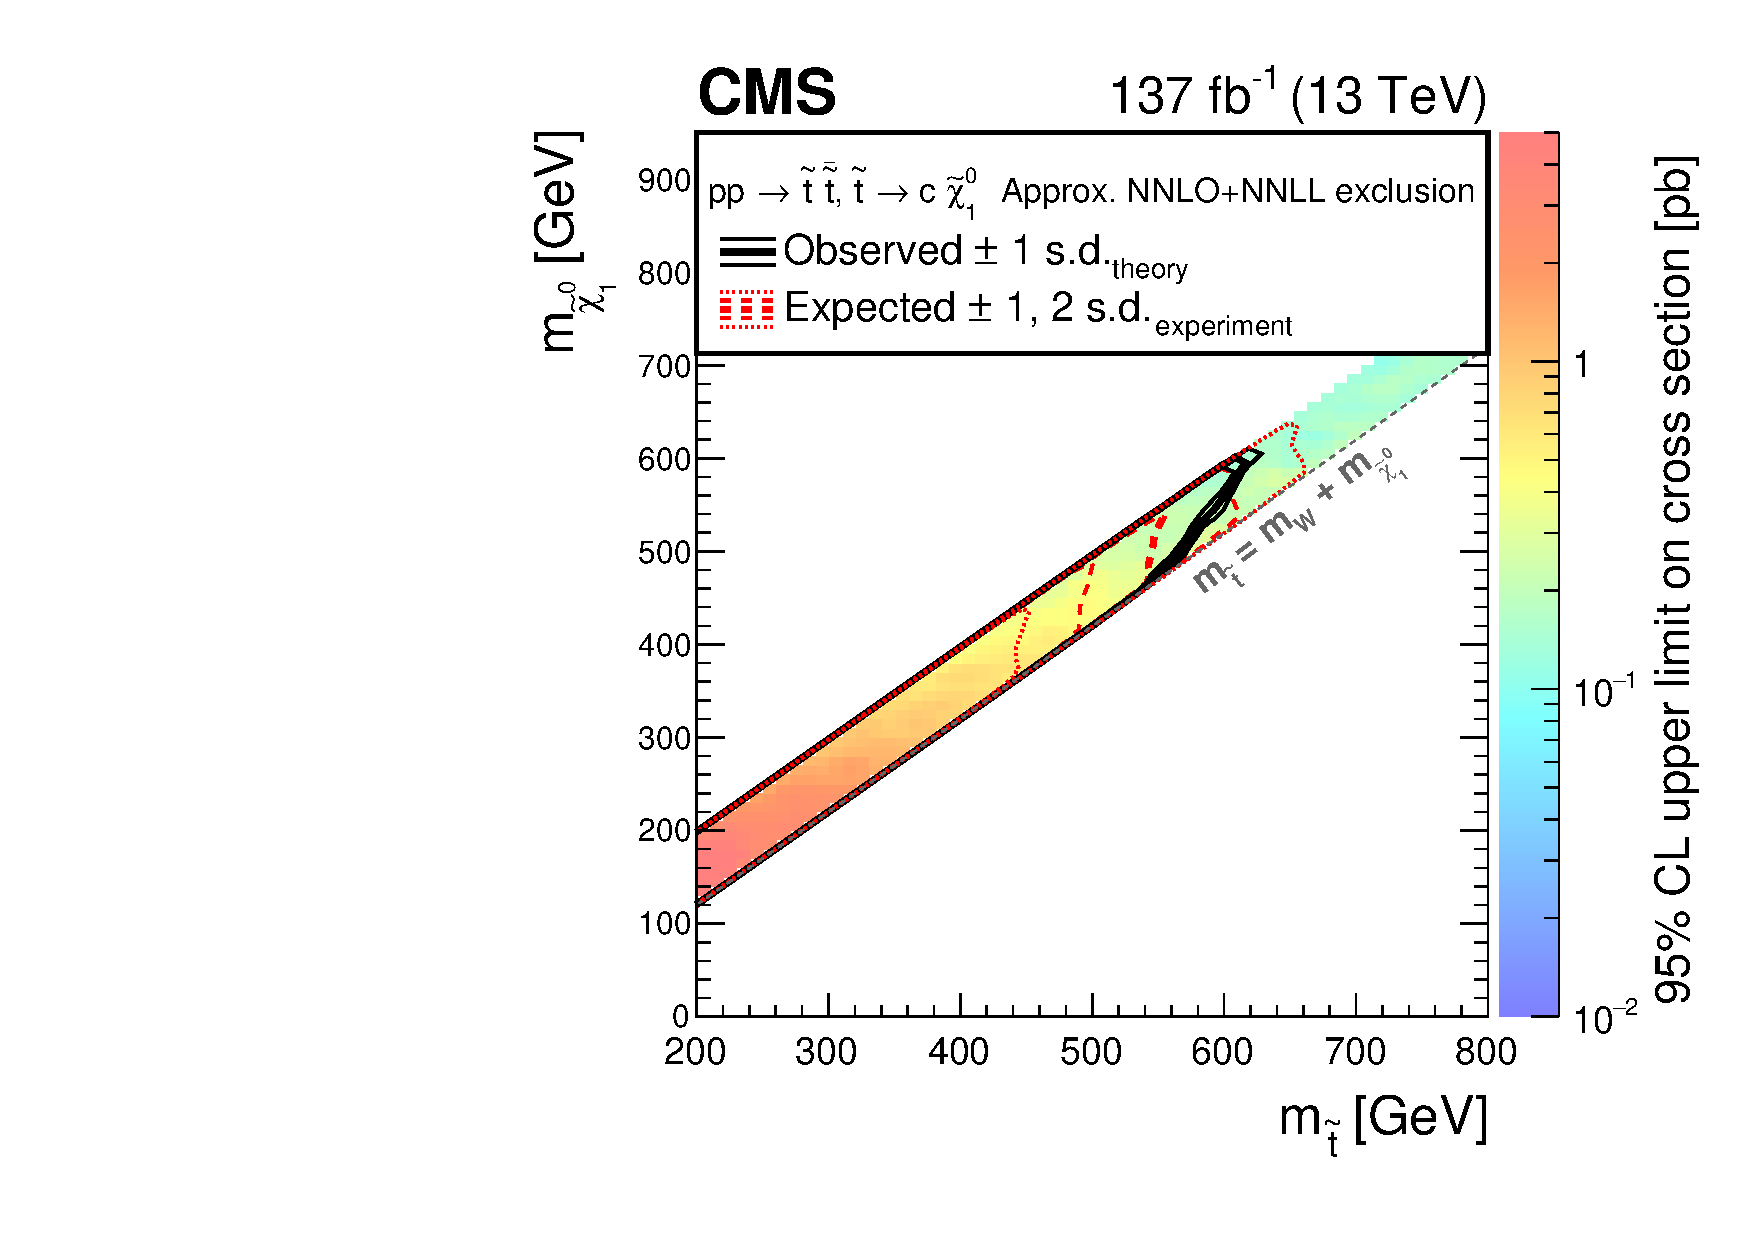
\includegraphics[width=0.49\textwidth]{figures/MT2_2019/Figure_014-c}
   \caption[Exclusion limit at 95\% \CL for top squark pair production for various decay modes of the top squark.]{
     Exclusion limits at 95\% \CL for top squark pair production and decay to (upper left) a bottom quark and \chargino, which subsequently decays to a W boson and \lsp, (upper right) either a bottom quark and \chargino or top quark and \lsp, or (lower) a charm quark and \lsp. Taken from \cite{MT2_2019}.}
   \label{fig:stop_other}
\end{figure*}

\begin{figure}[htbp]
 \centering
   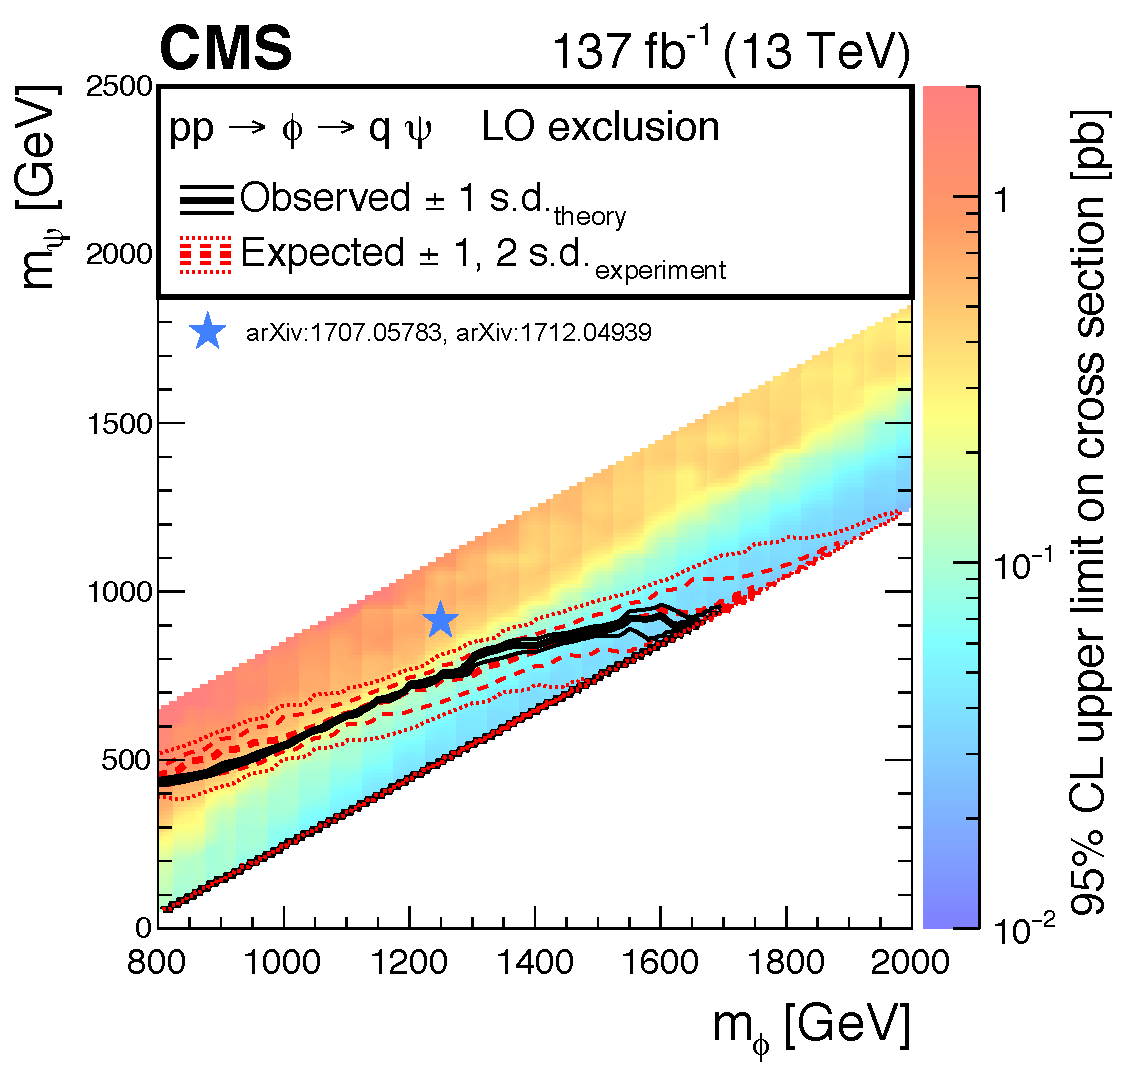
\includegraphics[width=0.49\textwidth]{figures/MT2_2019/Figure_015}
   \caption[Exclusion limit at 95\% \CL for the mono-$\phi$ model.]{
     Exclusion limit at 95\% \CL for the mono-$\phi$ model. 
     Only the portion of the mass plane of phenomenological interest was simulated.
     The star indicates the original authors' proposed best fit mass point, which remains unexcluded.
     Taken from \cite{MT2_2019}.}
   \label{fig:monophilimits}
\end{figure}

\begin{figure*}[htbp]
 \centering
   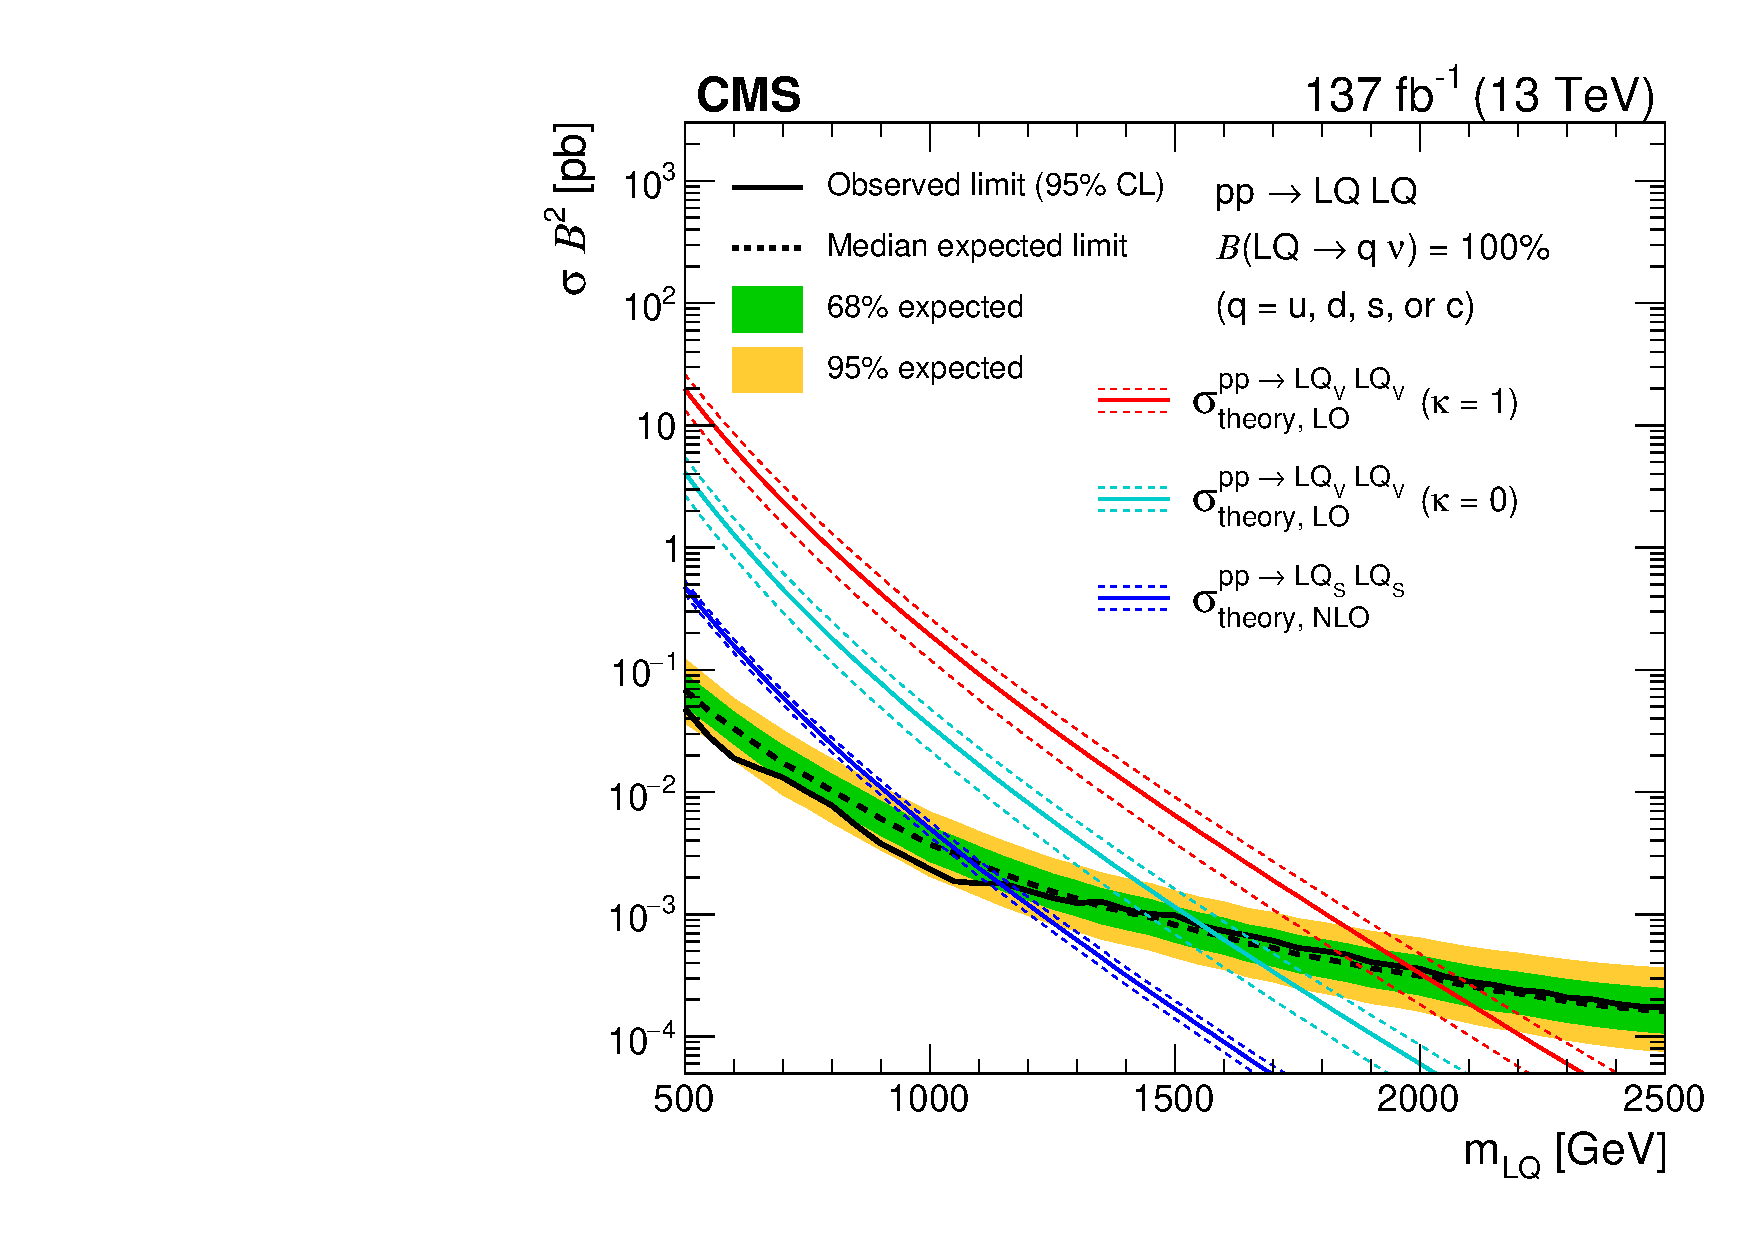
\includegraphics[width=0.49\textwidth]{figures/MT2_2019/Figure_016-a}
   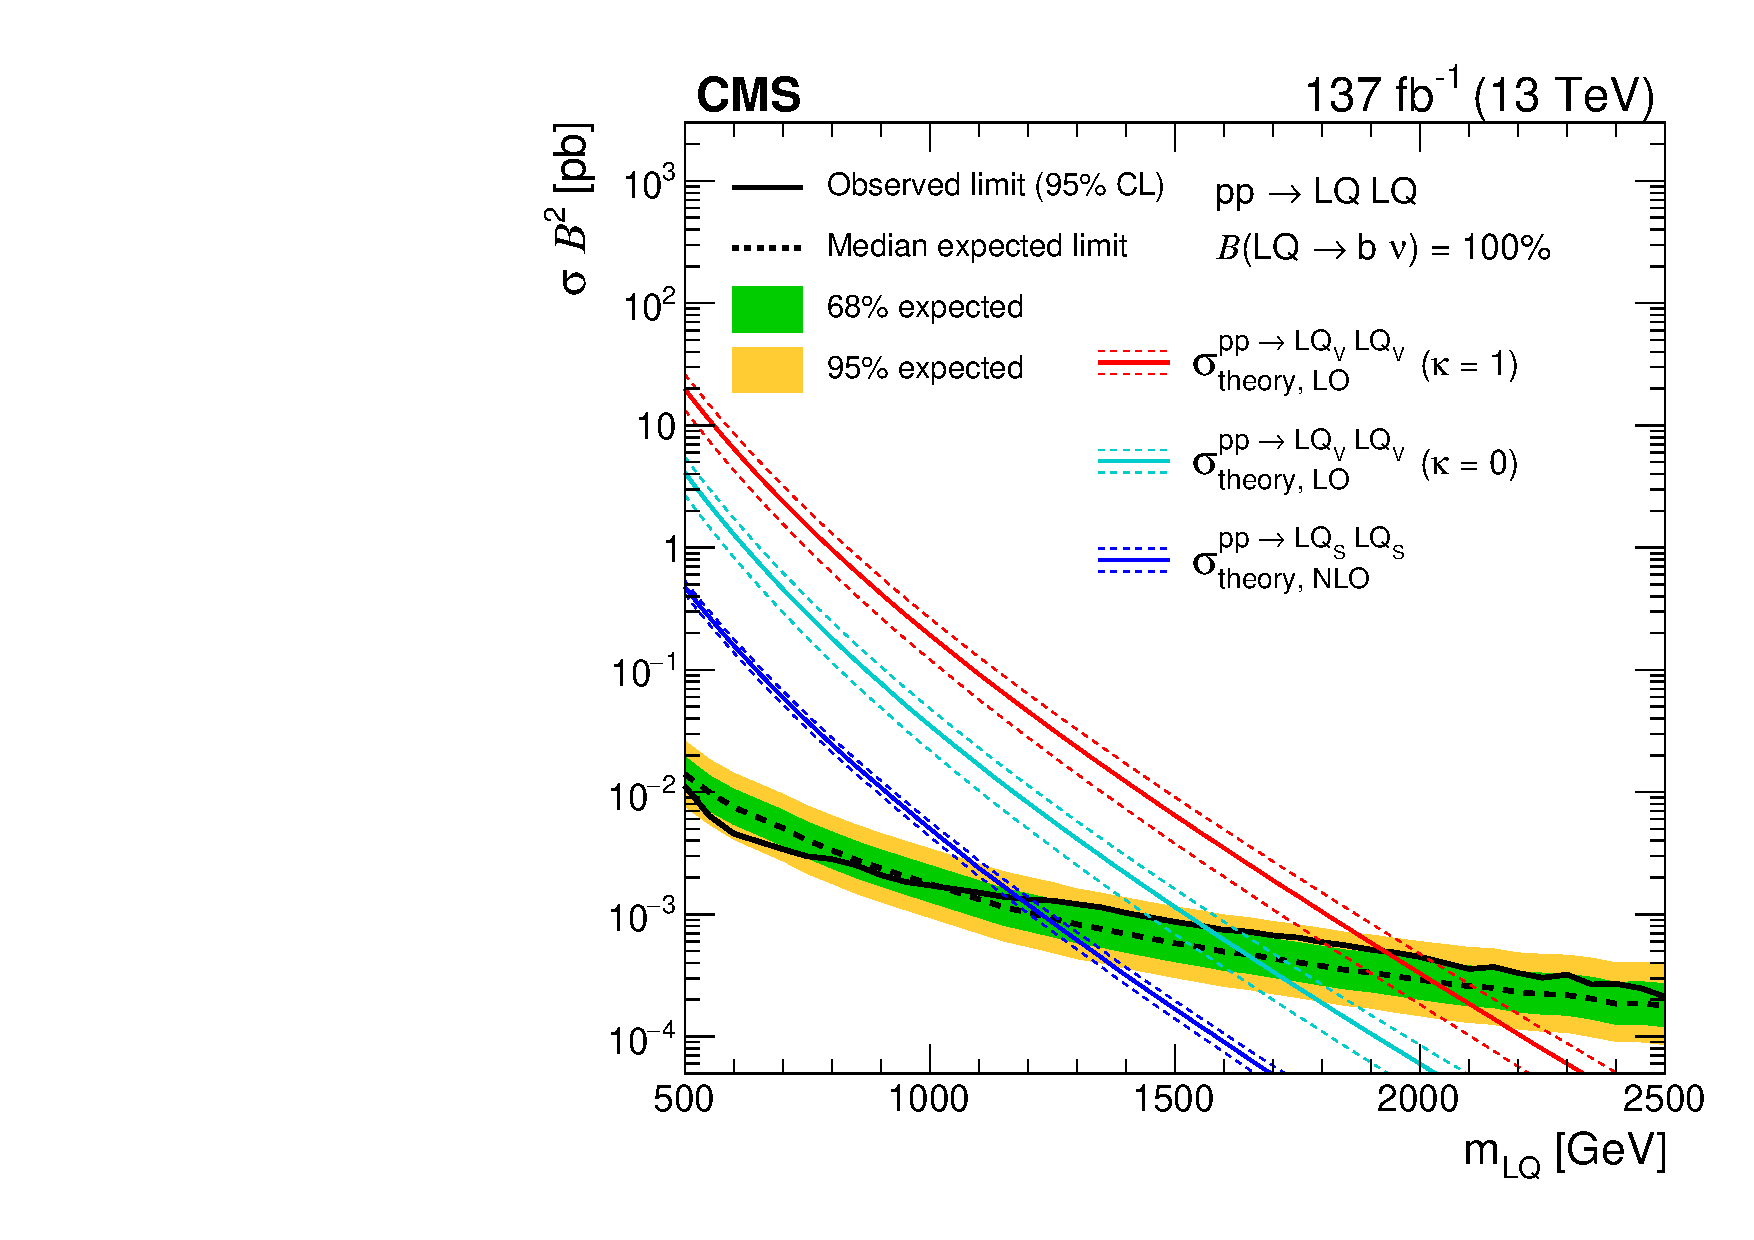
\includegraphics[width=0.49\textwidth]{figures/MT2_2019/Figure_016-b}
   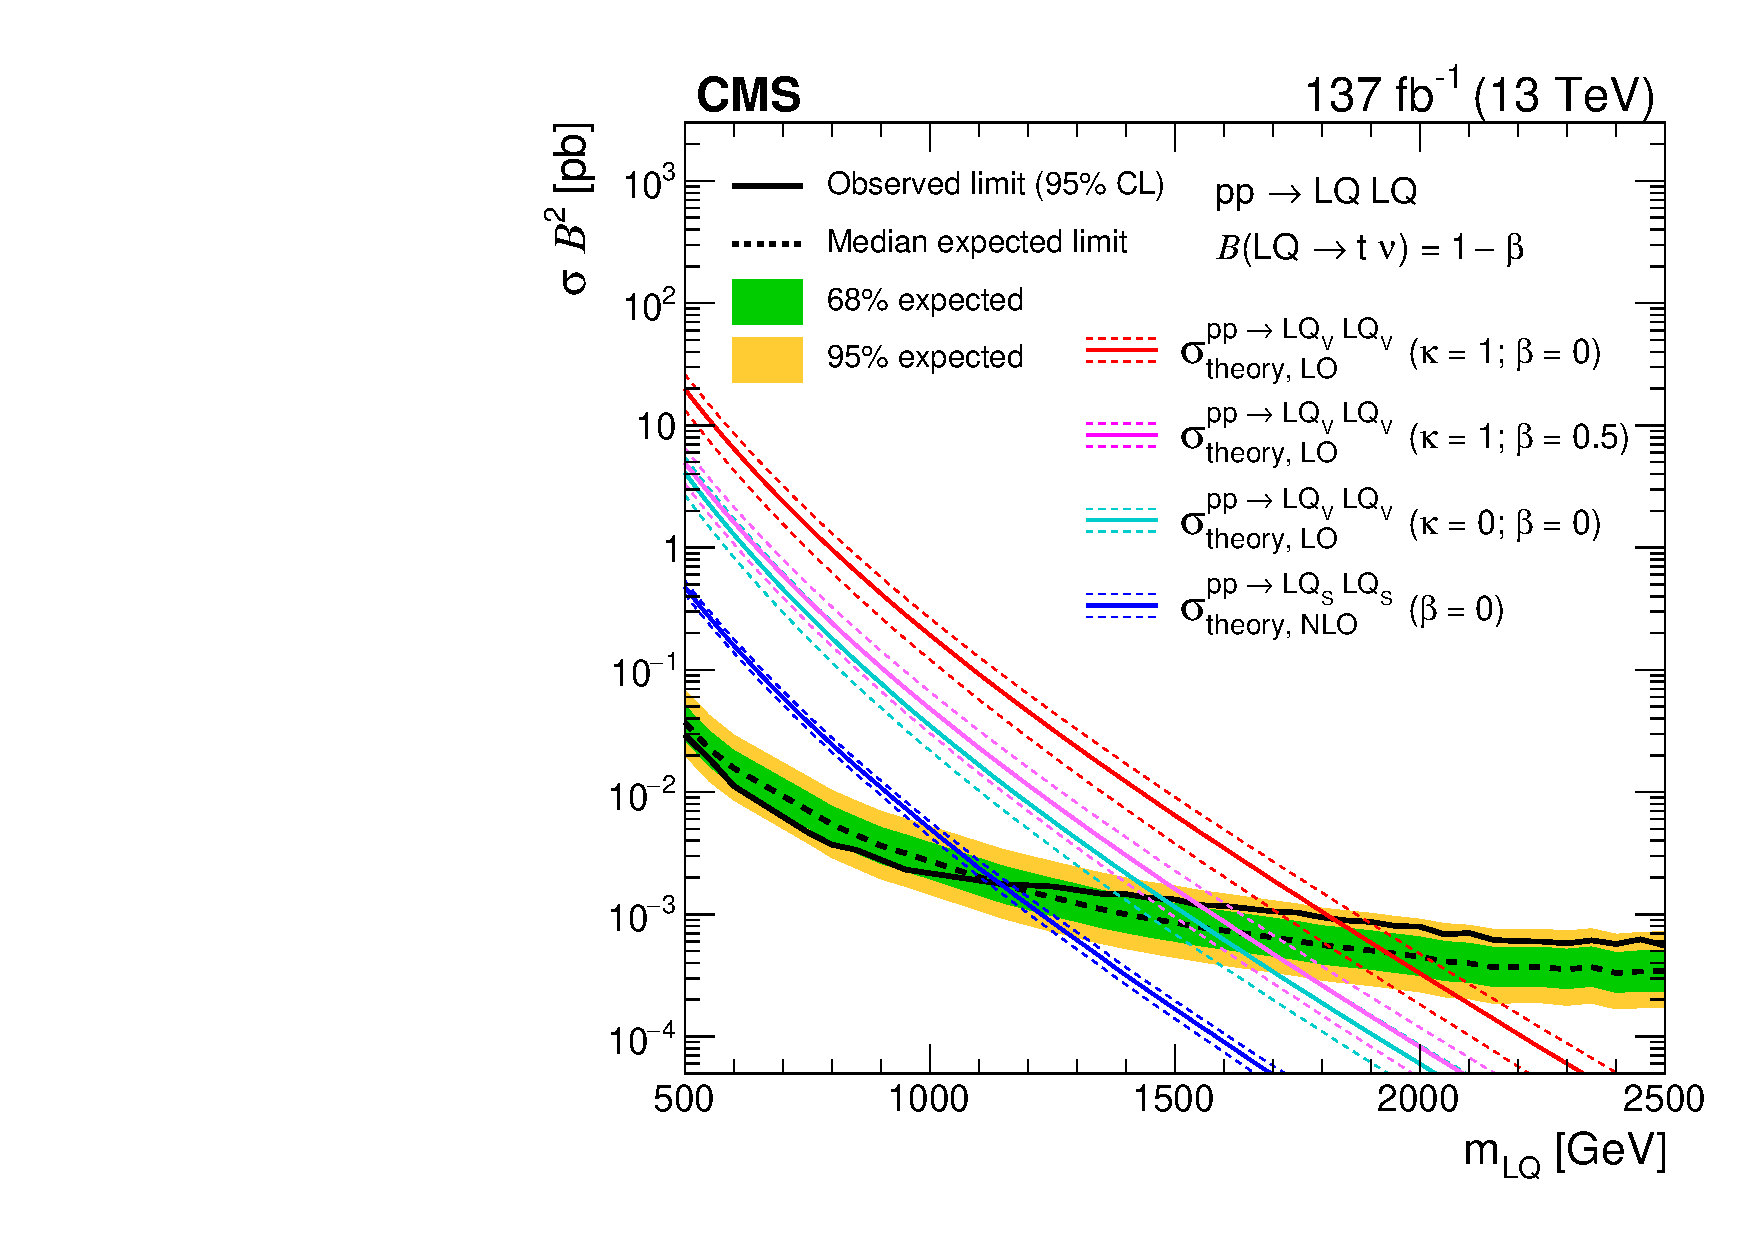
\includegraphics[width=0.49\textwidth]{figures/MT2_2019/Figure_016-c}
   \caption[Upper limits at 95\% \CL on the leptoquark production cross sections as a function of leptoquark mass.]{
     Upper limits at 95\% \CL on the leptoquark production cross sections as a function of leptoquark mass. 
     Unlike the limits on supersymmetric models, in which the mass of \lsp is a free parameter, the limits on leptoquarks are 1-dimensional in the leptoquark mass since the neutrino masses are known to be approximately zero.
     Taken from \cite{MT2_2019}.}
   \label{fig:lqlimit}
\end{figure*}

  Figure~\ref{fig:t5x} shows the exclusion curves for gluino pair production and decay to light quarks (upper), light quarks and the Z boson (lower left), and light quarks and the W boson (lower right).
  Figure~\ref{fig:t1x} shows the exclusion curves for gluino pair production and decay to bottom (left) and top (right) quarks.

  Figure~\ref{fig:t2x} shows the exclusion curves for light-flavor squark (upper left), bottom squark (upper right), and (lower) top squark pair production in which the top squark decays to a top quark. 
  The light-flavor figure contains two curves, one which assumes that there is only a single low mass light flavor squark, and another that assumes that there are eight light flavor squarks of (approximately) degenerate mass, which implies a production cross section eight times larger.
  The other top squark decay modes, in which the top decays to (upper left) a bottom quark and \chargino, which subsequently decays to a W boson and \lsp, (lower) a charm and \lsp, and (upper right) either \chargino and a bottom quark or \lsp and a top quark, are shown in Figure~\ref{fig:stop_other}.
  The charm decay channel is only shown for signal models with small mass splittings, as the top squark would strictly prefer to decay to a top quark and \lsp than to a charm quark and \lsp if kinematically allowed.

  Figure~\ref{fig:monophilimits} shows limits placed on the mono-$\phi$ model.
  Here, the horizontal axis is the mass of the singly-produced scalar $\phi$, and the vertical axis the mass of the invisible fermion $\psi$.
  A star indicates the mass point proposed by the original authors in \cite{monophi} as most phenomenologically interesting, which is not yet excluded.
  It is worth emphasizing that the background model is nevertheless consistent with data; this signal is simply very difficult to exclude with the \mttwo analysis methodology.
  To save computing resources, the mono-$\phi$ model is only simulated in the phenomenologically interesting subset of the mass plane, similarly to the top squark to charm model in Figure~\ref{fig:stop_other} (lower), hence the large white space beneath the considered range of masses.

  Figure~\ref{fig:lqlimit} shows limits for leptoquarks decaying to (upper left) a light flavor quark and neutrino, (upper right) a bottom quark and neutrino, and (lower) a top quark and neutrino.
  As the mass of the neutrinos, in contrast to the mass of \lsp, are known to be approximately zero, the leptoquark limits are one dimensional, in the leptoquark masses.

  The limits produced by this edition of the classic search improve upon the limits set by the previous edition \cite{MT2_2016} by hundreds of GeV, and in most cases are the strongest constraints on their respective signal models yet produced by any experiment.

  \subsection{Future of the Classic \mttwo Search} \label{sec:MT2future}

  The current limits produced by the classic \mttwo search are impressive, and are unlikely to improve much in the near future.
  The pair production cross section for squarks and gluinos drops rapidly with mass, as shown in Figure~\ref{fig:SUSYxsec}.
  Generically, a factor of 10 improvement in sensitivity is necessary to push the exclusion limits outward by around 500 GeV along the horizontal axis.
  At this mature statistical stage, a factor of 10 improvement in sensitivity requires a factor of 100 increase in the integrated luminosity, infeasible in the near future.
  Improvement along the \lsp axis is similarly difficult due to large backgrounds and low signal efficiency for models with small mass splittings.
  Therefore, attention in the near future will turn to other new techniques, one of which is discussed in the next section.

\section{Disappearing Tracks Search}

  \subsection{General Description} \label{sec:distracksdescription}

  Define a disappearing track.
  This search takes the very same events as the classic search, and adds a disappearing track requirement.

    \subsubsection{Motivation} \label{sec:distracksmotivation}

    Why are disappearing track searches interesting? (SUSY can make them, could have new physics right under our noses that we don't see because it looks weird, huge background suppression).

    \subsubsection{Challenges} \label{sec:distrackschallenges}

    Low statistics make it difficult to study background in detail, mysterious sources of background.

    \subsubsection{Signals} \label{sec:distrackssig}

    SMS diagrams. Mention that decay lengths can vary, and our sweet spot is decays in the track, 10-100 cm.
    Signal tends to be isolated, high quality.

    \subsubsection{Backgrounds} \label{sec:distracksbg}

    Electrons converting to photons, pions from taus, fakes, and strange baryons.
    Describe various cleaning selections.
    Suppress electrons by mapping and vetoing dead ECAL locations, suppress fakes with quality cuts, suppress strange baryons with HCAL energy veto.

  \subsection{Data-Driven Background Estimate} \label{sec:distracksbgest}

  Emphasize that MC should not be trusted to understand a background requiring such detailed detector knowledge.

    \subsubsection{Short Track Candidates and $f_{short}$} \label{sec:fshort}

    How do tracks disappear? Who knows: ask the data, for tracks that we are confident are not signal, and remain agnostic of the precise underlying causes.
    Crucial assumption that the ratio between signal-unlike and signal-like background is flat with MT2.

    \subsubsection{Validation} \label{sec:distracksvalidation}

    Check that background estimate is working at higher MT2, where signal still ought to be relatively rare.    

    \subsubsection{Signal Contamination} \label{sec:distrackssigcontam}

    Similar to the classic MT2 adjustment for lepton control region contamination, but two-layered.
    First, need to account for low MT2 ST contamination.
    Then, need to account for high MT2 STC contamination.
    Linearize (strictly conservative) so that correction scales appropriately with signal strength.

  \subsection{Results} \label{sec:distracksresults}

  Show final signal region results.
  No excesses, and potentially quote most discrepant bins.

  \subsection{Limits} \label{sec:distrackslimits}

  Refer to description of combine statistics procedure in classic search, and show limit scans.

  \subsection{Future} \label{sec:distracksfuture}

  Discuss that, due to small background, disappearing track search scales almost linearly with luminosity, and search is overall heavily dominated by statistical errors.
  May be worth pursuing in the future at 14 TeV.

%  \begin{figure}[h!]
%    \centering
%    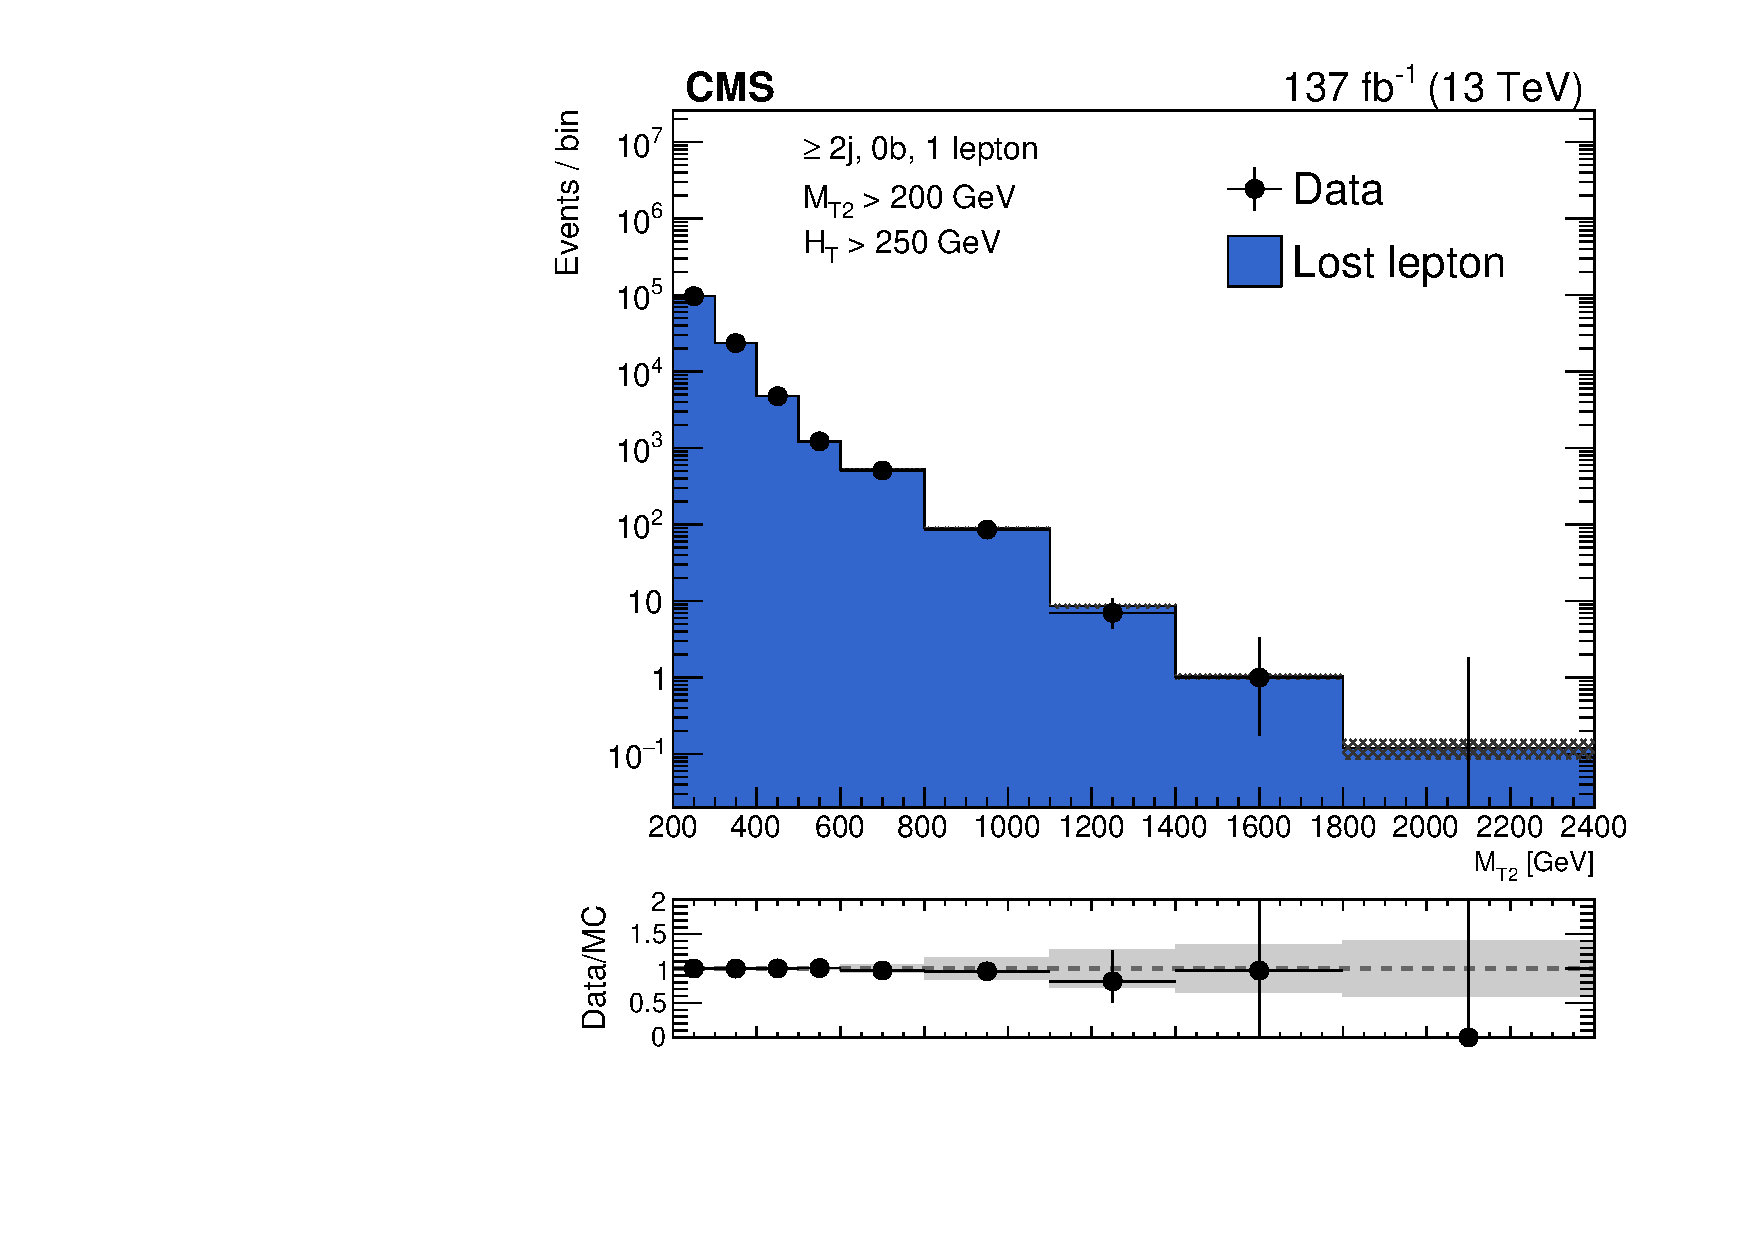
\includegraphics[width=0.48\textwidth]{figures/MT2_2019/Figure_001-a.pdf}
%    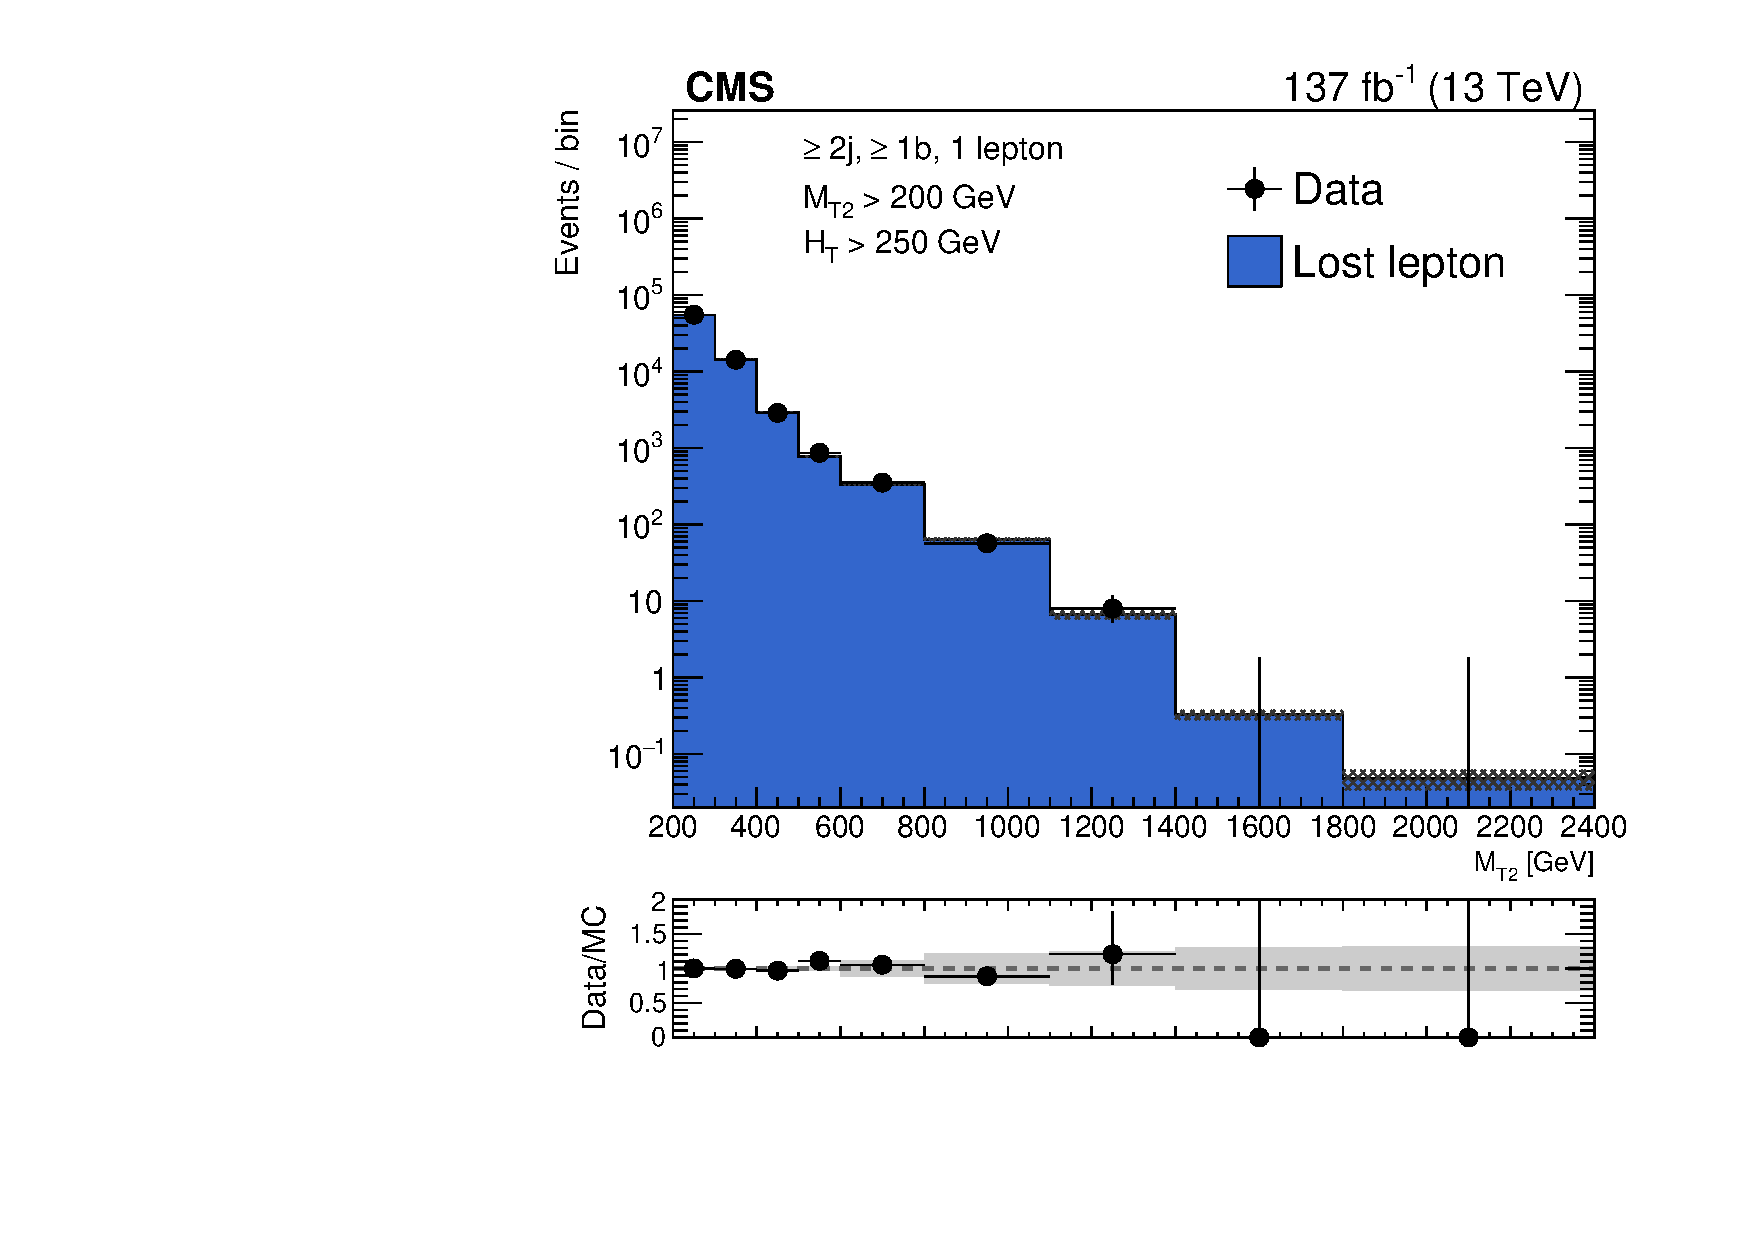
\includegraphics[width=0.48\textwidth]{figures/MT2_2019/Figure_001-b.pdf}
%    \caption[Distributions of \Mttwo in data and simulation for the single-lepton control region, to check \Mttwo modeling in simulation.]{Modeling of \Mttwo in simulation is checked against data with 0 (left) and 1 b-tagged jets, in events containing one lepton. Taken from \cite{MT2_2019}}
%    \label{fig:lepmt2}
%  \end{figure}  


  \begin{figure}[h!]
    \centering
    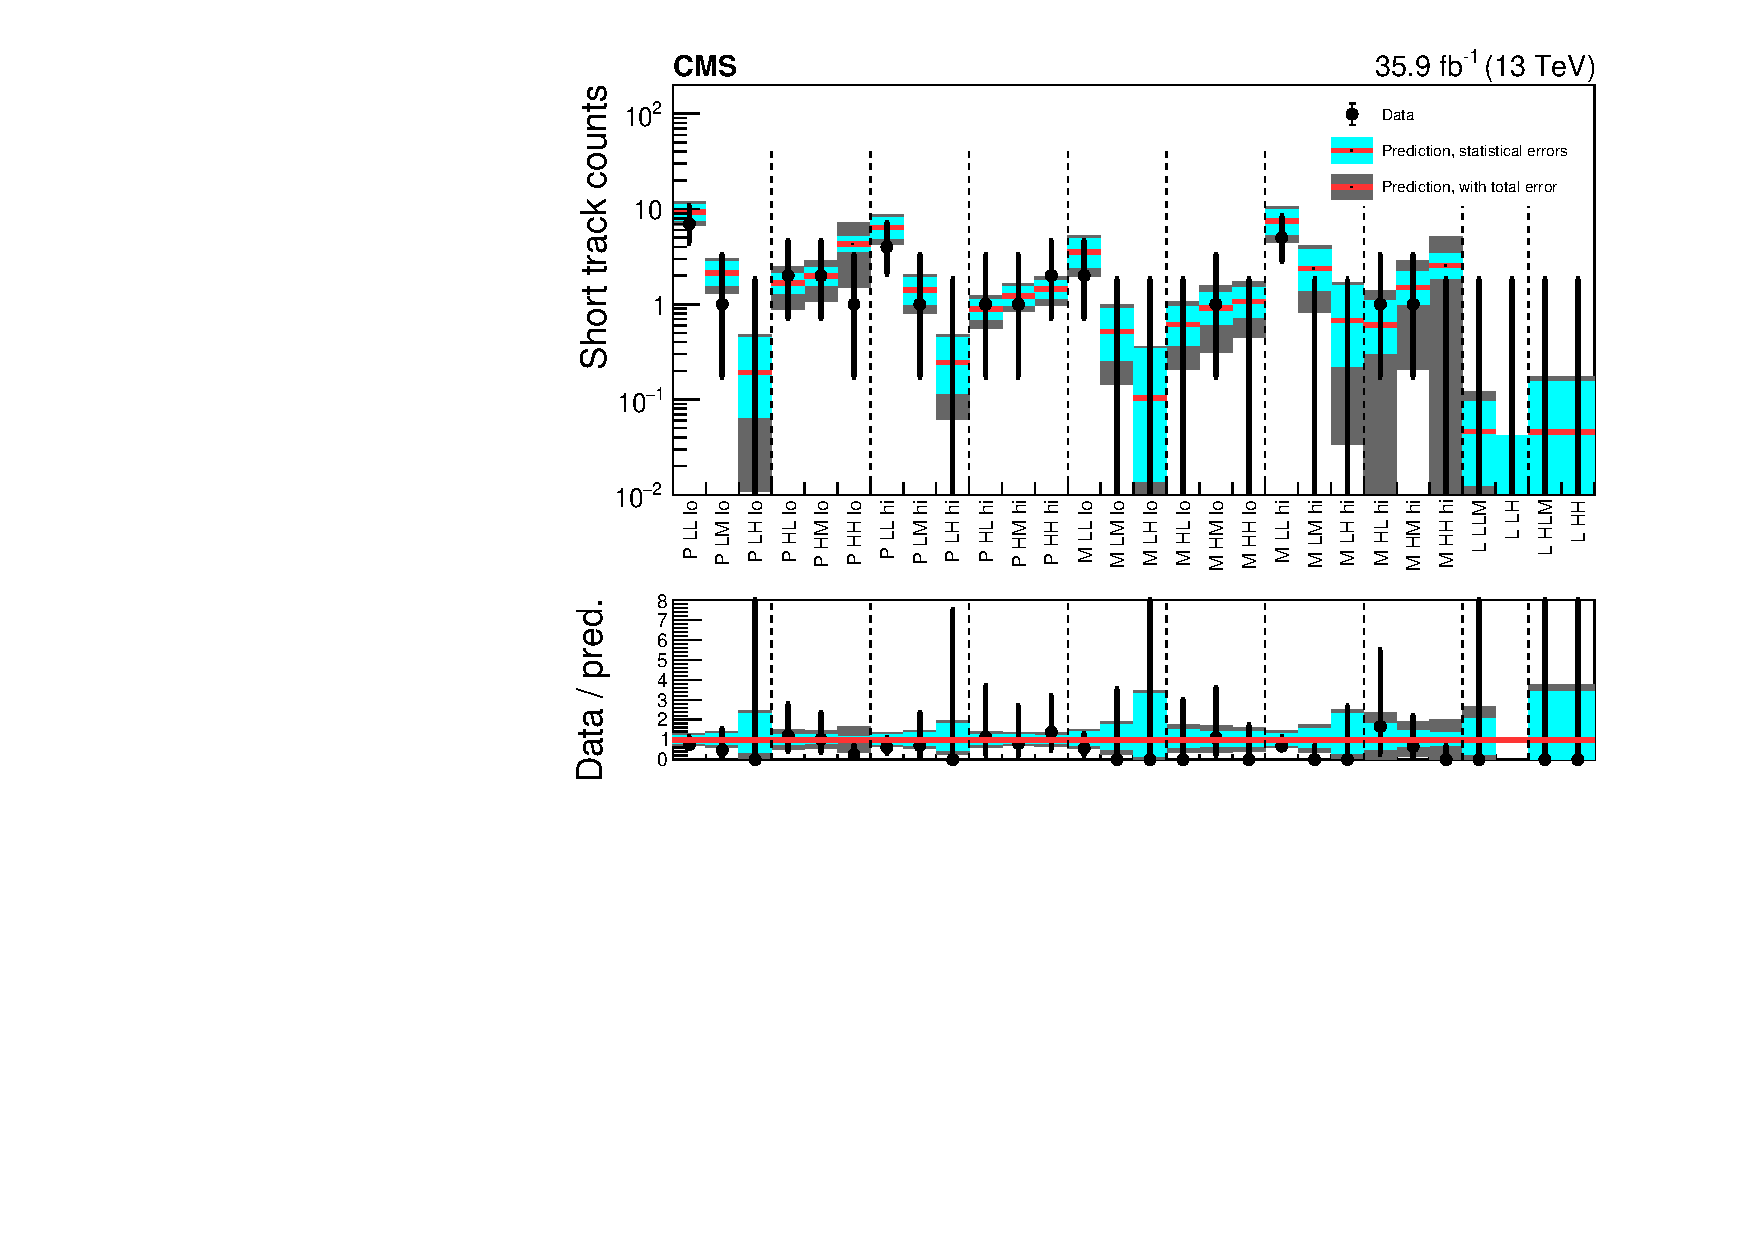
\includegraphics[width=0.85\textwidth]{figures/MT2_2019/Figure_004-a.pdf}
    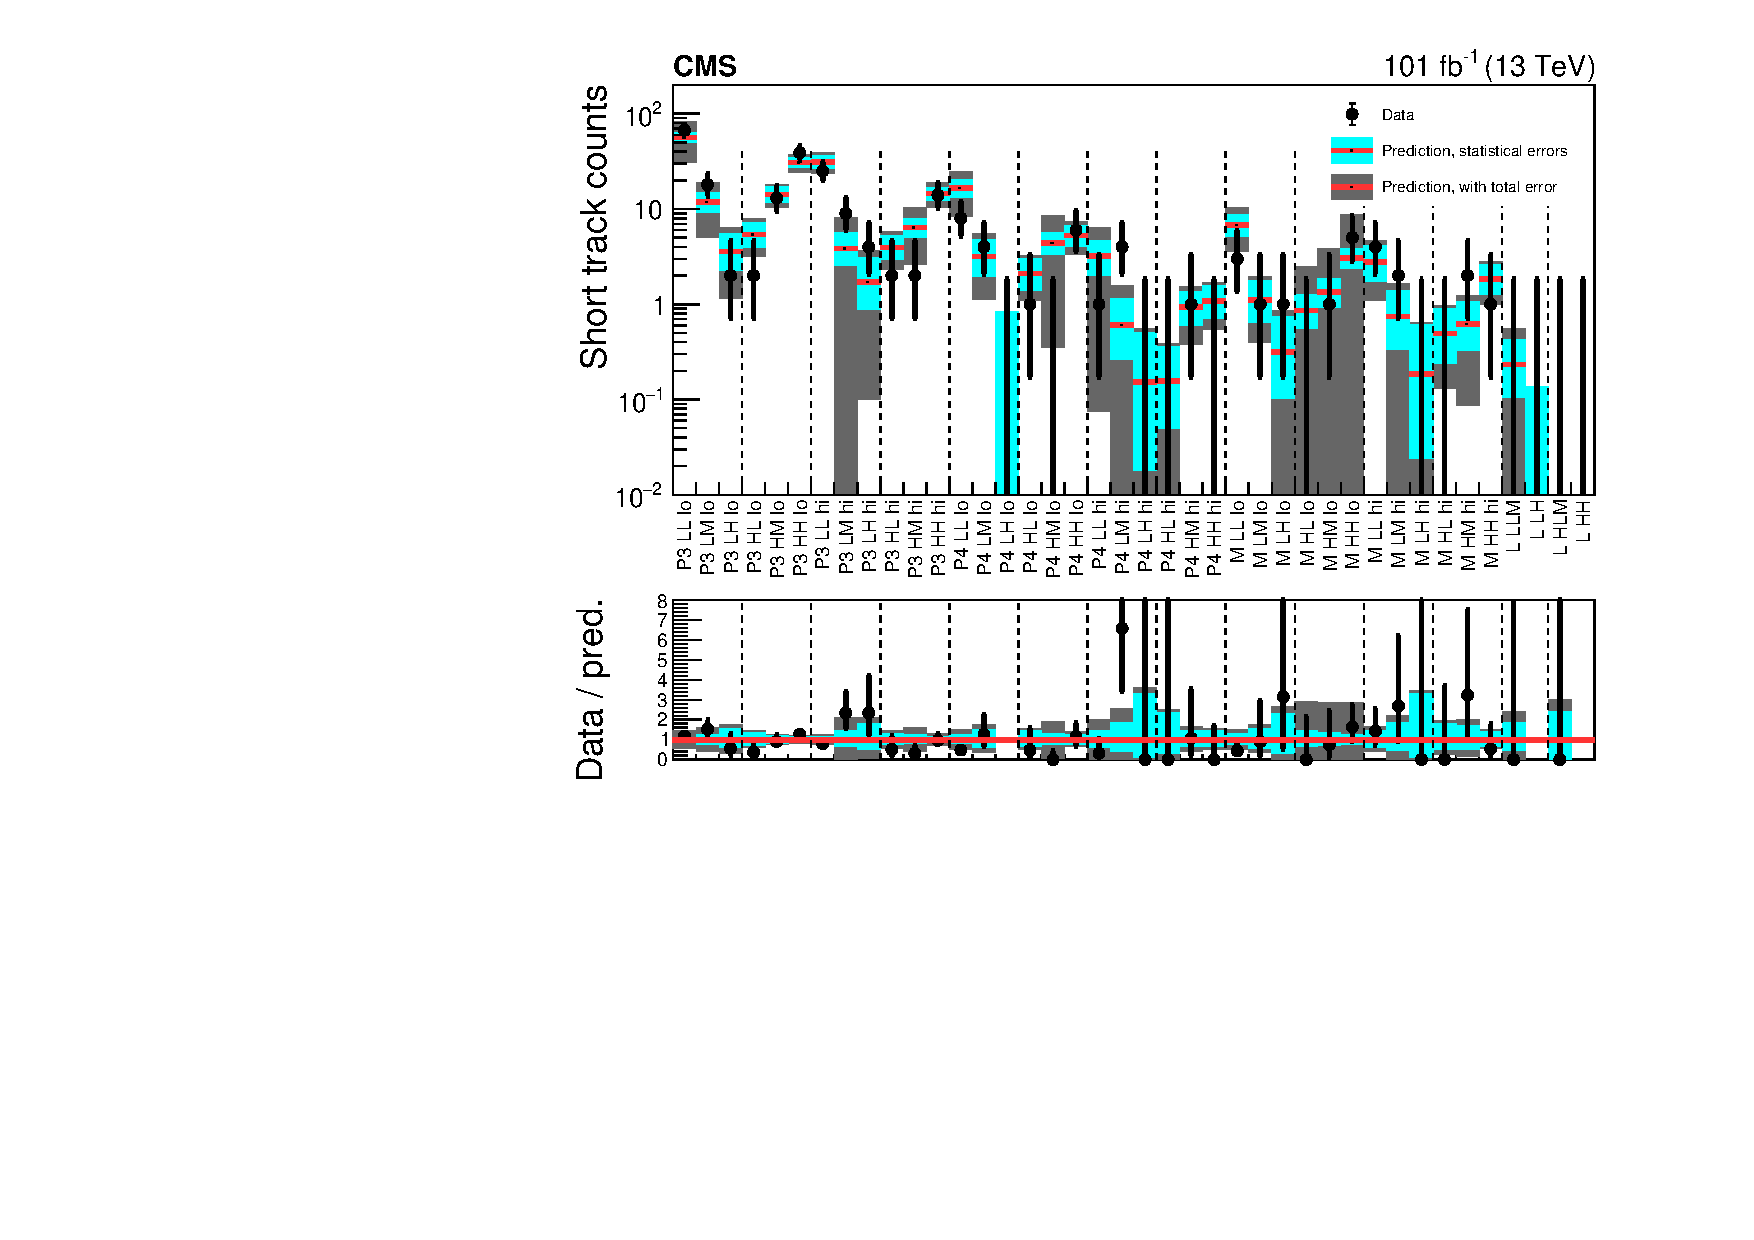
\includegraphics[width=0.85\textwidth]{figures/MT2_2019/Figure_004-b.pdf}
    \caption[Validation of the disappearing tracks background estimate in (upper) 2016 and (lower) 2017--2018 data.]{Taken from \cite{MT2_2019}}
    \label{fig:distracksval}
  \end{figure}  


  \begin{figure}[h!]
    \centering
    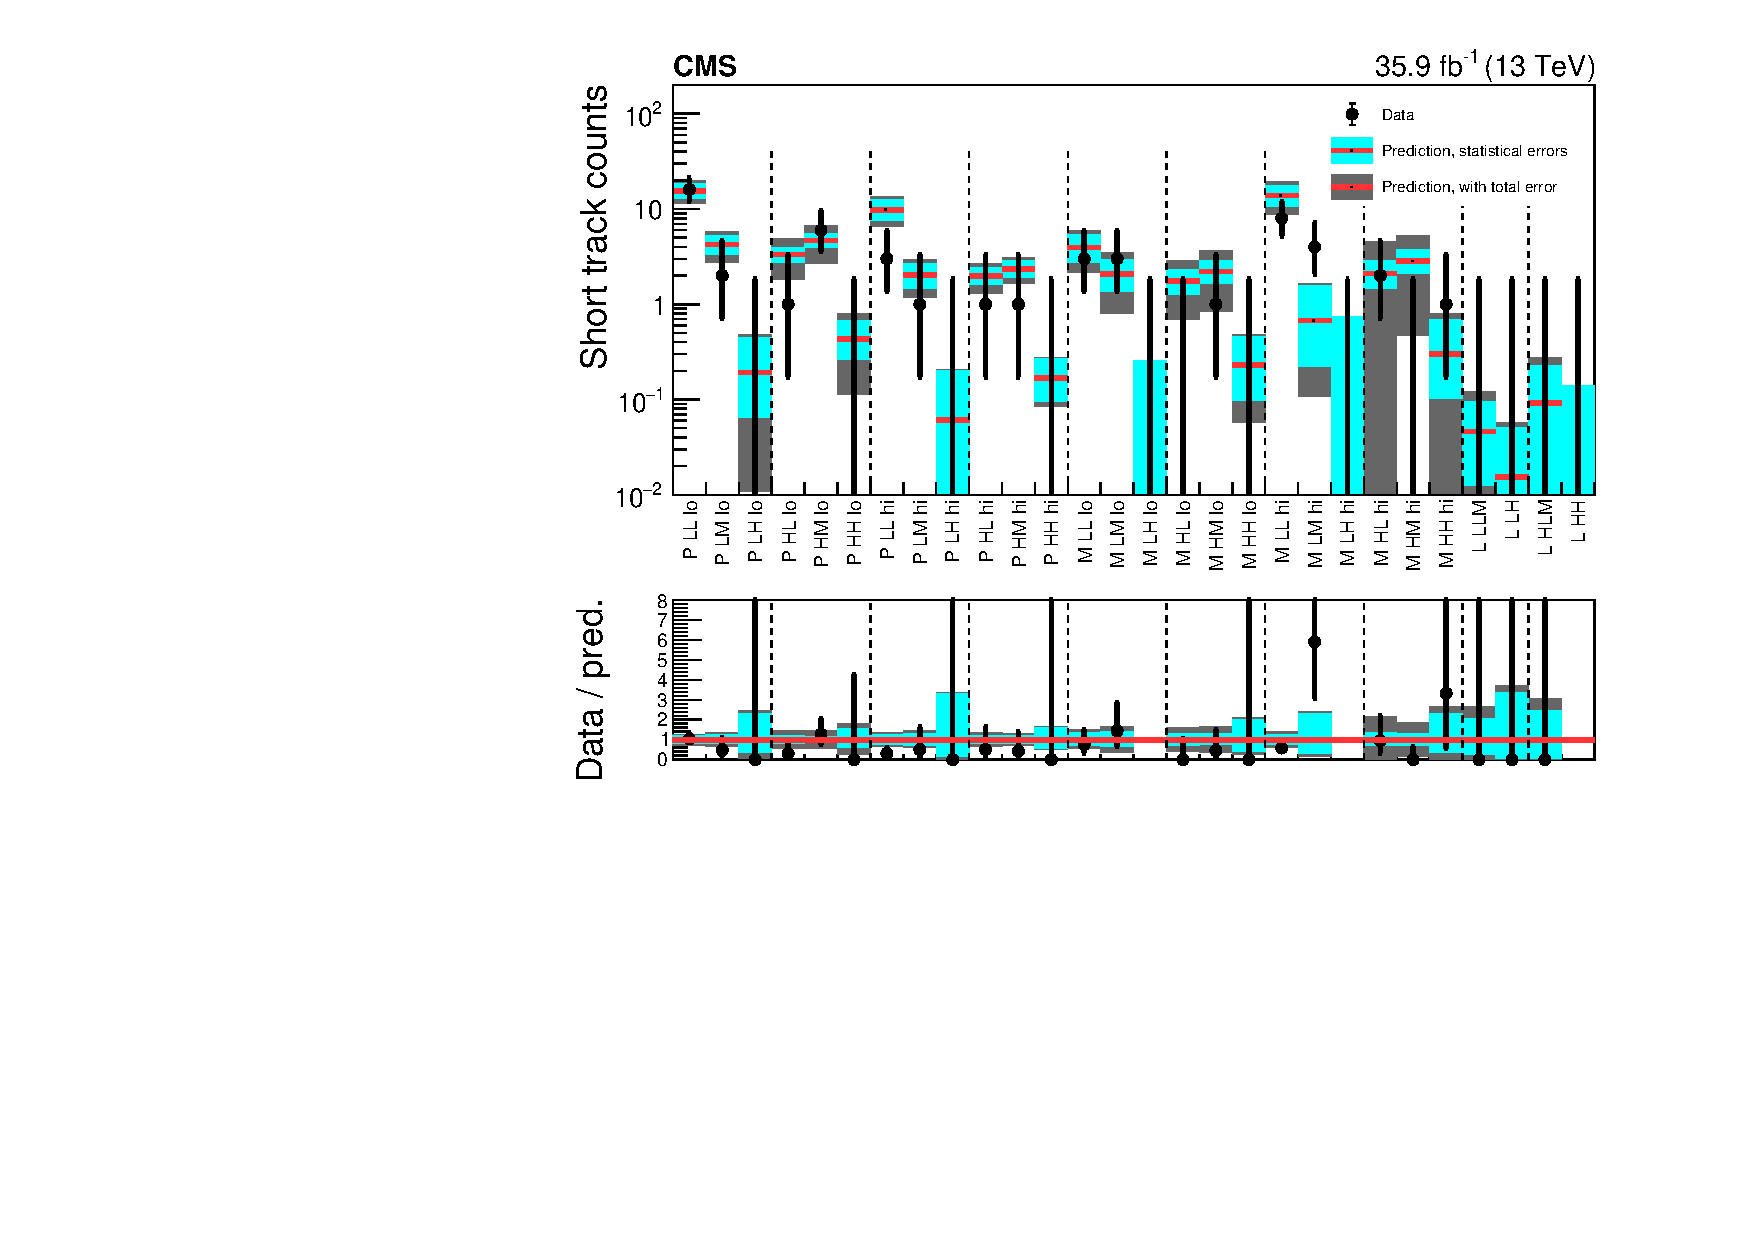
\includegraphics[width=0.85\textwidth]{figures/MT2_2019/Figure_006-a.pdf}
    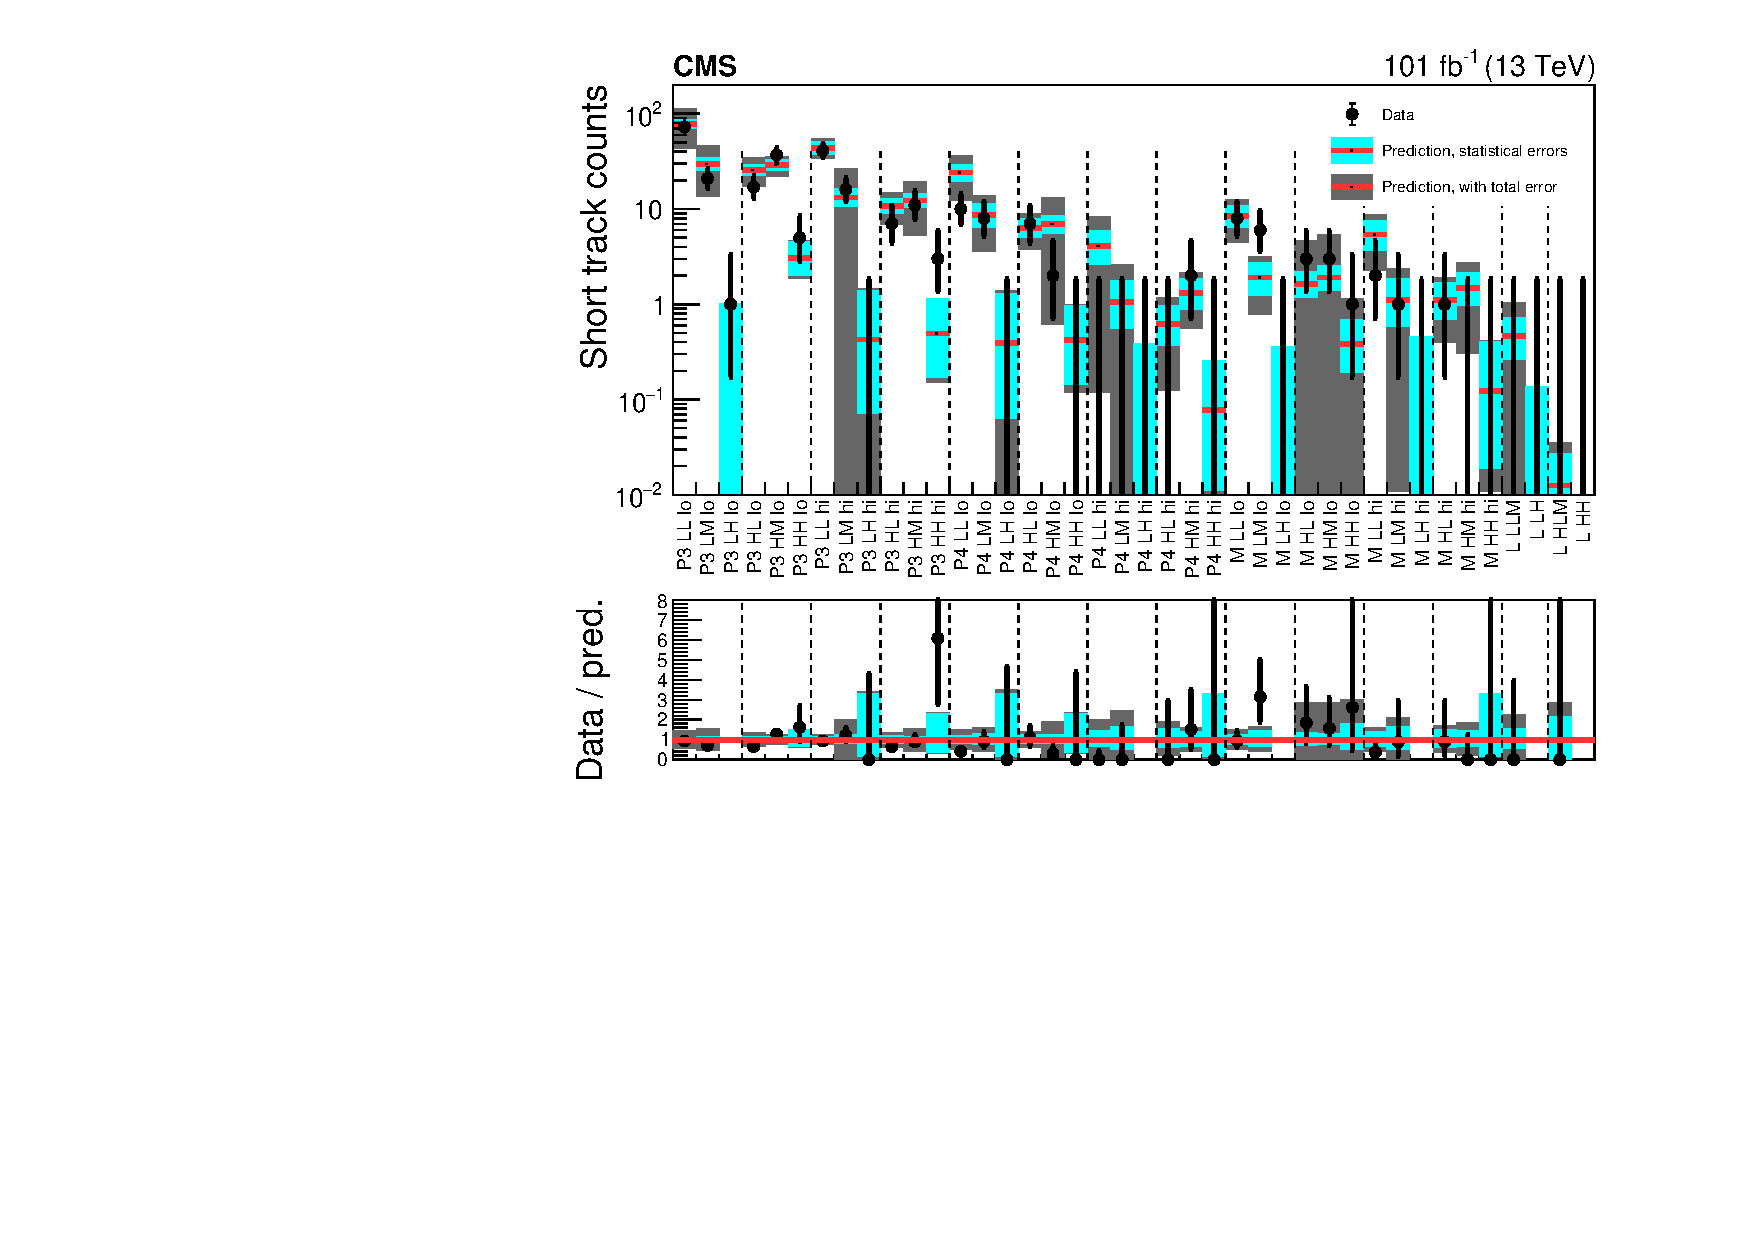
\includegraphics[width=0.85\textwidth]{figures/MT2_2019/Figure_006-b.pdf}
    \caption[Comparison of the predicted background and observed data events in the disappearing track search for (upper) 2016 and (lower) 2017--2018.]{Taken from \cite{MT2_2019}}
    \label{fig:distracksresults}
  \end{figure}  


\begin{figure*}[htbp]
  \centering
    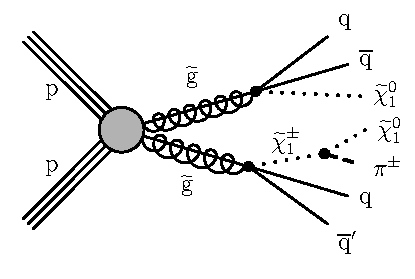
\includegraphics[width=0.3\textwidth]{figures/MT2_2019/Figure_010-a}
    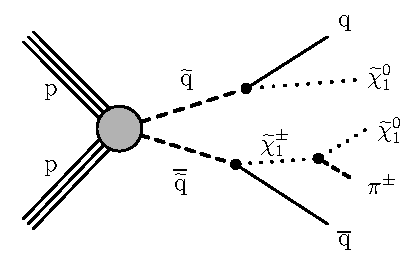
\includegraphics[width=0.3\textwidth]{figures/MT2_2019/Figure_010-b}
    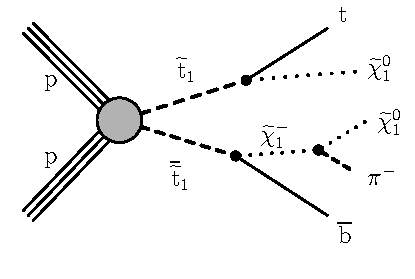
\includegraphics[width=0.3\textwidth]{figures/MT2_2019/Figure_010-c}
    \caption[Diagrams for (left) gluino, (center) light-flavor squark, and (right) top squark pair production, in which the gluinos and squarks can decay via a long-lived \chargino]{Diagrams for (left) gluino, (center) light-flavor squark, and (right) top squark pair production, in which the gluinos and squarks can decay via a long-lived \chargino. In this analysis, the gluino is taken to decay with branching fraction 1/3 each to the \lsp, \chargino plus, and \chargino minus. Squarks decay with branching fraction 1/2 each to the \lsp and the \chargino allowed by charge conservation. The \chargino mass is greater than the \lsp mass by hundreds of MeV, so that the charged product of the \chargino decay is too soft to be detected. Taken from \cite{MT2_2019}}
    \label{fig:charginodiags}
\end{figure*}



\begin{figure*}[htbp]
  \centering
    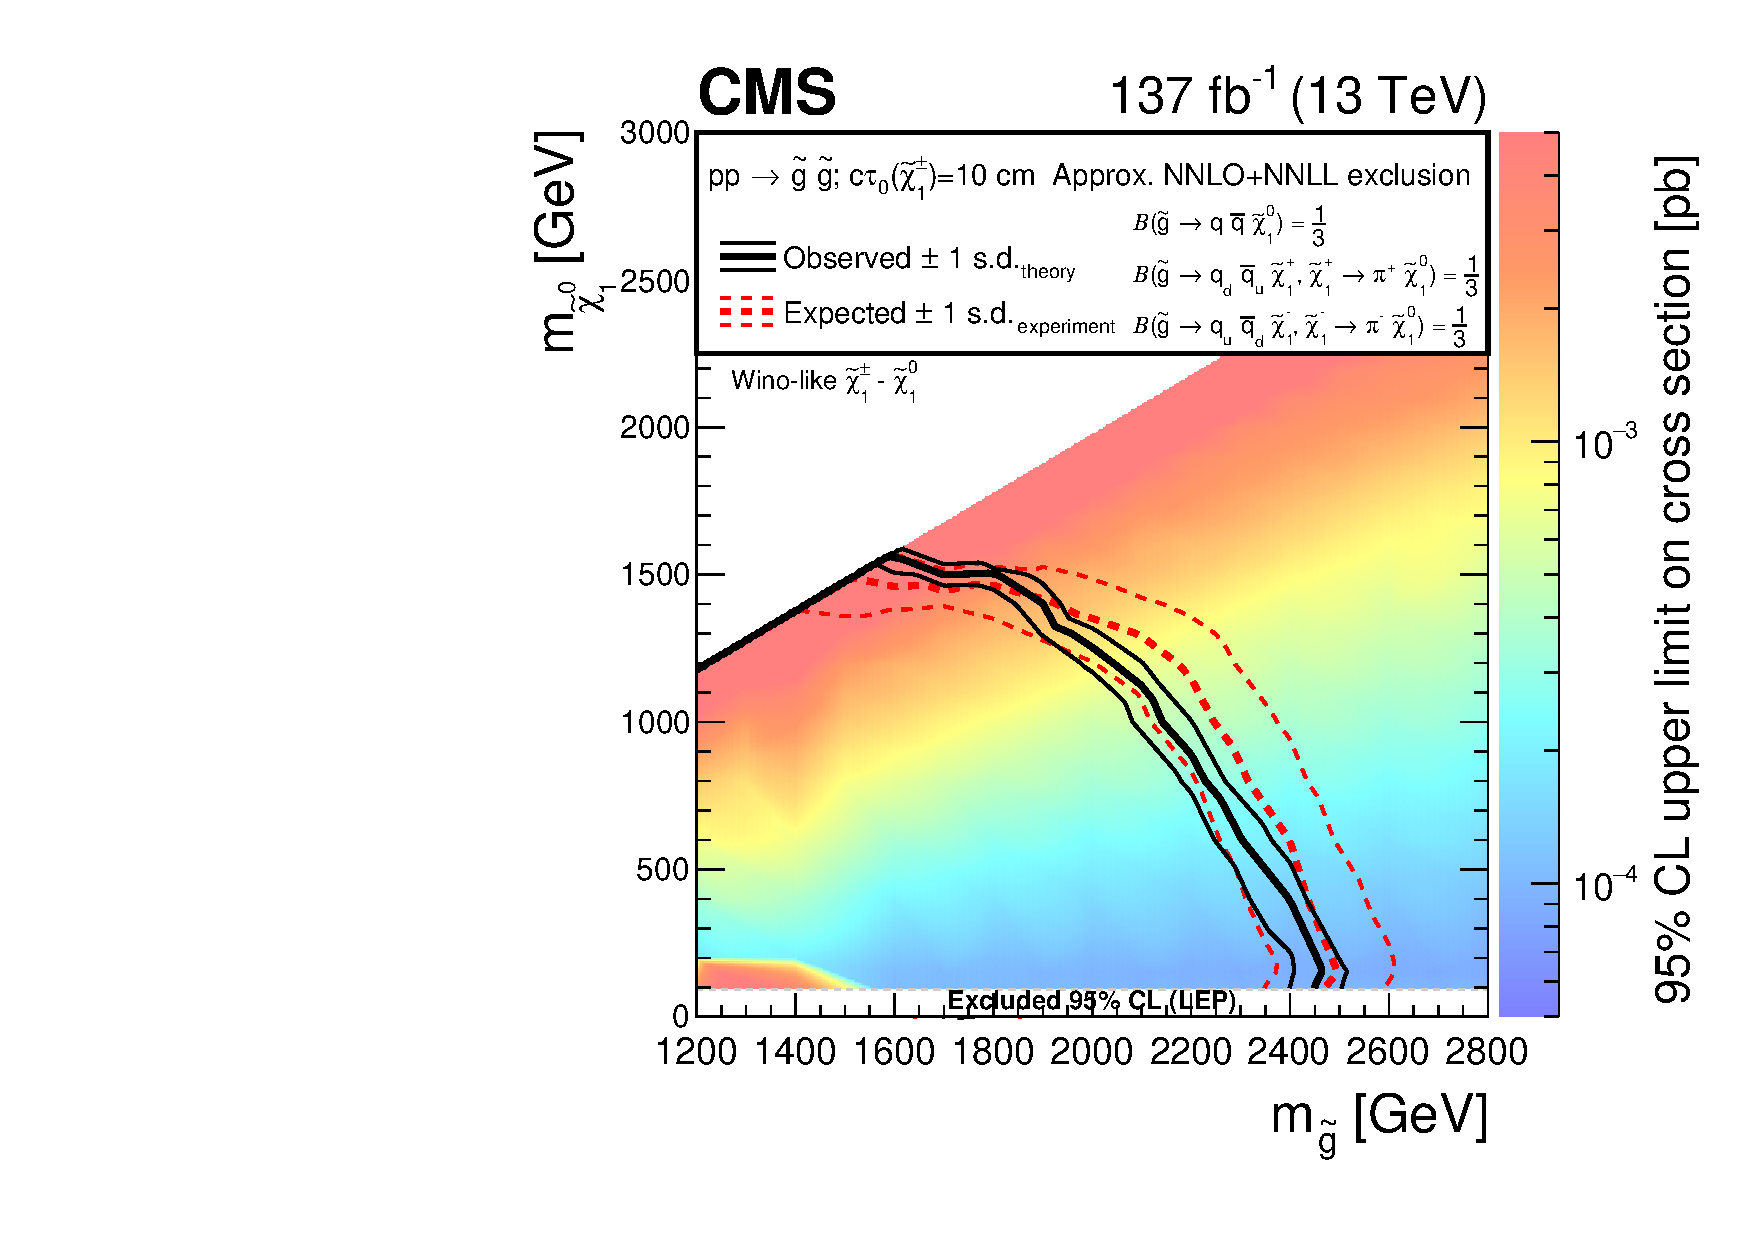
\includegraphics[width=0.48\textwidth]{figures/MT2_2019/Figure_017-a}
    \includegraphics[width=0.48\textwidth]{figures/MT2_2019/Figure_017-b}
    \includegraphics[width=0.48\textwidth]{figures/MT2_2019/Figure_017-c}
    \caption[Exclusion limits at  95\% \CL for direct gluino pair production where the gluinos decay to light-flavor quarks, with $c\tau_{0}(\chargino) =$ (upper left) 10\cm,
    (upper right) 50\cm, and (lower) 200\cm.]{Taken from \cite{MT2_2019}}
    \label{fig:t1st_qqqq}
\end{figure*}

\begin{figure*}[htbp]
  \centering
    \includegraphics[width=0.48\textwidth]{figures/MT2_2019/Figure_018-a}
    \includegraphics[width=0.48\textwidth]{figures/MT2_2019/Figure_018-b}
    \includegraphics[width=0.48\textwidth]{figures/MT2_2019/Figure_018-c}
    \caption[Exclusion limits at 95\% \CL for light squark pair production with $c\tau_{0}(\chargino) =$ (upper left) 10\cm, (upper right) 50\cm, and (lower) 200\cm.]{Taken from \cite{MT2_2019}}
    \label{fig:t2st_qq}
\end{figure*}

\begin{figure*}[htbp]
  \centering
    \includegraphics[width=0.48\textwidth]{figures/MT2_2019/Figure_019-a}
    \includegraphics[width=0.48\textwidth]{figures/MT2_2019/Figure_019-b}
    \includegraphics[width=0.48\textwidth]{figures/MT2_2019/Figure_019-c}
    \caption[Exclusion limits at 95\% \CL for top squark pair production with $c\tau_{0}(\chargino) =$ (upper left) 10\cm,
    (upper right) 50\cm, and (lower) 200\cm.]{Taken from \cite{MT2_2019}}
    \label{fig:t2st_tt}
\end{figure*}

\begin{figure*}[htbp]
  \centering
    \includegraphics[width=0.48\textwidth]{figures/MT2_2019/Figure_020-a}\\
    \includegraphics[width=0.48\textwidth]{figures/MT2_2019/Figure_020-b}
    \includegraphics[width=0.48\textwidth]{figures/MT2_2019/Figure_020-c}
    \caption[Exclusion limits at  95\% \CL on the \lsp mass, with $m_{\chargino}=m_{\lsp}+\mathcal{O}(100\MeV)$, as a function of the \chargino proper decay length,
    for (upper) direct gluino and (lower) direct light-flavor squark pair production, for representative gluino and squark masses.]{Taken from \cite{MT2_2019}}
    \label{fig:limits1fixedmass}
\end{figure*}

\begin{figure}[htb!]
  \centering
    \includegraphics[width=0.48\textwidth]{figures/MT2_2019/Figure_021}
    \caption[Exclusion limits at  95\% \CL on the \lsp mass, with $m_{\chargino}=m_{\lsp}+\mathcal{O}(100\MeV)$, as a function of the \chargino proper decay length,
    for  direct top squark pair production, as obtained for a representative top squark mass.]{Taken from \cite{MT2_2019}}
    \label{fig:limits1fixedmass_stop}
\end{figure}

\begin{figure*}[htbp]
  \centering
    \includegraphics[width=0.48\textwidth]{figures/MT2_2019/Figure_022-a}\\
    \includegraphics[width=0.48\textwidth]{figures/MT2_2019/Figure_022-b}
    \includegraphics[width=0.48\textwidth]{figures/MT2_2019/Figure_022-c}
    \caption[Exclusion limits at  95\% \CL on $\sigma/\sigma_{\mathrm{theory}}$ as a function of the \chargino decay length, for
    (upper) gluino pair production where the gluinos decay to light-flavor quarks, (lower left) light-flavor squark pair production,
    and (lower right) top squark pair production, as obtained from the search for disappearing tracks.]{Taken from \cite{MT2_2019}}
    \label{fig:limits2fixedmasses}
\end{figure*}
